%
%
%
%
%
%
\PassOptionsToPackage{svgnames,dvipsnames}{xcolor} %
\documentclass[acmsmall,screen,nonacm]{acmart}

%
\acmJournal{CSUR}
\acmYear{2026}\acmVolume{1}\acmNumber{1}\acmArticle{1}\acmMonth{1}
\settopmatter{authorsperrow=3}      %
%

%
\usepackage{forest}
\useforestlibrary{edges}   %
\usepackage{tikz}
\usetikzlibrary{arrows.meta,positioning,fit,backgrounds,shapes.geometric,calc}
\usepackage{pifont}

%
\newcommand{\yy}{\textcolor{ForestGreen}{\ding{52}}}      %
\newcommand{\nn}{\textcolor{BrickRed}{\ding{56}}}         %
\newcommand{\dm}{\textcolor{gray!65}{\textbf{--}}}         %
\usepackage{longtable}
\usepackage{array}      %
\usepackage{placeins}   %

%
\newcommand{\tcode}{\textcolor{cat-code!55!black}{\textsf{\textbf{code}}}}
\newcommand{\tweights}{\textcolor{cat-vla!45!black}{\textsf{\textbf{weights}}}}
\newcommand{\treward}{\textcolor{cat-rew!55!black}{\textsf{\textbf{reward}}}}
\newcommand{\tskill}{\textcolor{cat-skill!45!black}{\textsf{\textbf{skill}}}}
\newcommand{\tpolicy}{\textcolor{cat-trans!55!black}{\textsf{\textbf{policy}}}}
\newcommand{\tbench}{\textcolor{cat-bench!45!black}{\textsf{\textbf{bench}}}}
%
\newcommand{\dreal}{\textcolor{ForestGreen}{\textsf{real}}}
\newcommand{\dsim}{\textcolor{RoyalBlue}{\textsf{sim}}}
\newcommand{\dgame}{\textcolor{Purple}{\textsf{game}}}
\newcommand{\dtext}{\textcolor{gray!70}{\textsf{text}}}
%
\newcommand{\flatent}{\textcolor{secA!45!black}{\textsf{latent-RL}}}
\newcommand{\fspace}{\textcolor{secB!45!black}{\textsf{skill-space}}}
\newcommand{\fcodelib}{\textcolor{secF!45!black}{\textsf{code-lib}}}
\newcommand{\fagent}{\textcolor{secG!45!black}{\textsf{agent-lib}}}
\newcommand{\pp}{\textcolor{orange!90!black}{\textbf{\textasciitilde}}}  %

%
%
%
%
%
%
%
%

%
\definecolor{hidden-draw}{RGB}{40,40,40}
\definecolor{tx-root}{HTML}{D1D5DB}

%
\definecolor{cat-code}{HTML}{93C5FD}\definecolor{leaf-code}{HTML}{DBEAFE}   %
\definecolor{cat-vla}{HTML}{5EEAD4}\definecolor{leaf-vla}{HTML}{CCFBF1}     %
\definecolor{cat-rew}{HTML}{FDBA74}\definecolor{leaf-rew}{HTML}{FEEBC8}     %
\definecolor{cat-skill}{HTML}{C4B5FD}\definecolor{leaf-skill}{HTML}{EDE9FE} %
\definecolor{cat-trans}{HTML}{F9A8D4}\definecolor{leaf-trans}{HTML}{FCE7F3} %
\definecolor{cat-bench}{HTML}{86EFAC}\definecolor{leaf-bench}{HTML}{DCFCE7} %

%
\definecolor{secA}{HTML}{93C5FD}\definecolor{secAl}{HTML}{DBEAFE} %
\definecolor{secB}{HTML}{5EEAD4}\definecolor{secBl}{HTML}{CCFBF1} %
\definecolor{secC}{HTML}{86EFAC}\definecolor{secCl}{HTML}{DCFCE7} %
\definecolor{secD}{HTML}{FCD34D}\definecolor{secDl}{HTML}{FEF3C7} %
\definecolor{secE}{HTML}{FCA5A5}\definecolor{secEl}{HTML}{FEE2E2} %
\definecolor{secF}{HTML}{C4B5FD}\definecolor{secFl}{HTML}{EDE9FE} %
\definecolor{secG}{HTML}{F9A8D4}\definecolor{secGl}{HTML}{FCE7F3} %

%
\forestset{
  default preamble={
    forked edges,
    for tree={
      grow=east,
      reversed=true,
      anchor=base west,
      parent anchor=east,
      child anchor=west,
      base=center,
      font=\large,
      rectangle,
      draw=hidden-draw,
      rounded corners,
      align=center,
      text centered,
      minimum width=5em,
      edge+={darkgray, line width=1pt},
      s sep=3pt,
      inner xsep=2pt,
      inner ysep=3pt,
      line width=0.8pt,
      ver/.style={rotate=90, child anchor=north, parent anchor=south, anchor=center},
      %
      if level=1{text width=19em, font=\normalsize}{},
      if level=2{text width=33em, font=\normalsize}{},
    },
  },
}
 
\begin{document}

\title{Weights or Skills?}
\subtitle{A Survey of Robot-Learning Techniques: from Action-Predicting
  Weights to Robots that Write their Own Skills}

\author{Gaytri Jena}
\affiliation{\institution{UC Berkeley}\city{Berkeley}\state{CA}\country{USA}}
\author{Kapil Wanaskar}
\affiliation{\institution{Canva Research}\country{USA}}
\author{Vinija Jain}
\affiliation{\institution{Google}\country{USA}}
\author{Aman Chadha}
\affiliation{\institution{Google DeepMind}\country{USA}}
\author{Vasu Sharma}
\affiliation{\institution{PocketFM}\country{USA}}
\author{Amitava Das}
\affiliation{\institution{Pragya Lab, BITS Pilani Goa}\country{India}}

\renewcommand{\shortauthors}{Jena et al.}

%
\begin{abstract}
Robot learning is splitting into two bets: policies that bake competence into \emph{frozen
weights} (vision-language-action, or VLA, models), and agents that write and refine their own
\emph{executable skills} as code. This survey organises the field around that axis of
\textbf{weights versus skills}. Its central analytical contribution is a deep-dive that arranges
code-as-policy methods by their \emph{degree of self-improvement}, from zero-shot program
synthesis, through closed-loop self-repair and persistent skill memory, to the sparsely
populated cell in which execution feedback, skill memory, and evolutionary search combine into
one open-ended loop; only a few very recent systems (for example ASPIRE, ENPIRE, and RoboClaw)
occupy that cell. We map the complementary ``skills'' pole, from unsupervised
reinforcement-learning skill discovery to large-language-model skill libraries, and show that
the word ``skill'' is used in at least five distinct senses, of which only the code sense
self-improves without gradient updates. We then connect the taxonomy to the emerging
\emph{skill economy}: commercial robot-skill marketplaces now distribute one-tap skills across
robots but ship only static playback, which surfaces open problems of adaptation,
cross-embodiment portability, provenance, safety verification, composition, and
standardisation. This is a deliberately \emph{focused} survey. Rather than cataloguing the
field exhaustively, it examines 77 representative systems across six technique families through
one taxonomy and a set of contrast tables, and it supplies operational definitions of the
self-improvement mechanisms together with a statement of what each family cannot do.
\end{abstract}
 
\begin{CCSXML}
<ccs2012>
   <concept>
       <concept_id>10010147.10010178.10010224</concept_id>
       <concept_desc>Computing methodologies~Robotic planning</concept_desc>
       <concept_significance>500</concept_significance>
   </concept>
   <concept>
       <concept_id>10010147.10010257</concept_id>
       <concept_desc>Computing methodologies~Machine learning</concept_desc>
       <concept_significance>300</concept_significance>
   </concept>
</ccs2012>
\end{CCSXML}
\ccsdesc[500]{Computing methodologies~Robotic planning}
\ccsdesc[300]{Computing methodologies~Machine learning}

\keywords{robot learning, code-as-policy, self-improvement, vision-language-action
  models, skill libraries, physical AI, survey}

\maketitle

%
\section{Introduction}
\label{sec:intro}

Two paradigms now dominate robot learning. \emph{Vision-language-action} (VLA)
models predict actions from frozen weights; \emph{code-as-policy} agents instead
write executable programs and improve them from experience~\citep{codeaspolicies,aspire}.
This survey is organised around that fault line.

\paragraph{Why now: the skill stack.}
The app store for robot skills has arrived; Unitree UniStore ships one-tap,
cross-model motion downloads~\citep{unistore2026}. But every skill in it is
\emph{static playback}: the least-capable point in the taxonomy. The skill stack has
three layers: \textbf{(1) Build} (how skills are created, \S\ref{sec:taxonomy}--\S\ref{sec:techniques}),
\textbf{(2) Distribute} (marketplaces and hubs), and \textbf{(3) Adapt} (on-device
self-improvement, \S\ref{sec:code}). UniStore is layer~2 over static layer-1 skills;
the promised value, ``adjust grip per fruit so nothing bruises'', lives in layer~3,
which no shipped skill does today.

\paragraph{Scope and contributions.}
This is a \emph{focused} survey rather than an exhaustive census. We examine 77 systems chosen
to populate a single analytical taxonomy, and we exclude pure perception, navigation, and
locomotion work except where it bears directly on how a manipulation skill is authored and
improved. Our contributions are: (i) a taxonomy organised by \emph{weights vs.\ skills}
(\S\ref{sec:taxonomy}); (ii) a deep-dive that arranges code-as-policy by \emph{degree of
self-improvement}, with operational definitions of the feedback, memory, and search mechanisms
and necessary-and-sufficient conditions for each rung (\S\ref{sec:code}); (iii) a map of the
``skills'' pole together with an analysis of the five senses in which ``skill'' is used
(\S\ref{sec:skill}); (iv) a summary of the characteristic strengths and limitations of each
technique family; and (v) an open-problems agenda for the emerging skill economy
(\S\ref{sec:open}). To situate these systems within the wider field,
Appendix~\ref{sec:landscape} (Table~\ref{tab:landscape}) catalogues 225 further representative
works, compared on six axes and grouped by area, bringing the survey's total coverage to more than
three hundred works.

\paragraph{Related surveys.}
Table~\ref{tab:survey_compare} contrasts the topical coverage of the closest surveys with
ours, and Figure~\ref{fig:surveys} places them on a timeline. Within \emph{ACM Computing
Surveys} the nearest are on world models, embodied intelligence, and language-model
navigation, and beyond it a cluster covers vision-language-action models and foundation models
for manipulation; but none organises code-as-policy by degree of self-improvement or names
the \S3.1.5 cell.
%
%
\begin{table}[t]
\centering
\footnotesize
\renewcommand{\arraystretch}{1.25}
\begin{tabular}{@{}p{0.24\textwidth}c c *{6}{c}@{}}
\toprule
\textbf{Survey} & \textbf{Venue} & \textbf{Yr}
 & \tweights{} & \tcode{} & \tskill{} & \treward{}
 & \textcolor{secE!55!black}{\textbf{Self-impr.}} & \textcolor{cat-bench!45!black}{\textbf{Economy}}\\
\midrule
World Models~\cite{survey_worldmodels} & CSUR & 2025 & \pp & \nn & \nn & \nn & \nn & \nn\\
Embodied Intelligence~\cite{survey_embodiedintel}& CSUR & 2025 & \pp & \nn & \pp & \nn & \nn & \nn\\
Navigation via FLM~\cite{survey_navigation} & CSUR & 2026 & \pp & \pp & \nn & \nn & \nn & \nn\\
VLA for Embodied AI~\cite{survey_vla} & arXiv & 2024 & \yy & \nn & \nn & \nn & \nn & \nn\\
Large-VLM VLA~\cite{survey_vlmvla} & arXiv & 2025 & \yy & \nn & \nn & \pp & \nn & \nn\\
Embodied Learning~\cite{survey_embodiedlearn} & MIR & 2025 & \pp & \nn & \pp & \pp & \nn & \nn\\
FM for Manipulation~\cite{survey_fmrobot} & arXiv & 2024 & \yy & \pp & \pp & \pp & \nn & \nn\\
\midrule
\textbf{Ours (\emph{Weights or Skills?})} & \dm & 2026 & \yy & \yy & \yy & \yy & \yy & \yy\\
\bottomrule
\end{tabular}
\caption{Topical coverage of the closest related surveys versus ours.
\yy\ covered, \pp\ partial/mentioned, \nn\ not covered. Columns: \tweights{} (VLA/weights),
\tcode{} (code-as-policy), \tskill{} (skill libraries), \treward{} (reward synthesis),
\textbf{Self-impr.}\ (organised by \emph{degree of self-improvement}, incl.\ the \S3.1.5 cell),
\textbf{Economy} (the robot skill marketplace). Only this survey covers the last two axes.
CSUR = ACM Computing Surveys; MIR = Machine Intelligence Research.}
\label{tab:survey_compare}
\end{table}
 %
%
%
%
\begin{figure*}[p]
\centering
\resizebox{!}{0.88\textheight}{%
\begin{forest}
  for tree={align=center},
  where n children=0{font=\footnotesize, align=left}{font=\normalsize},
  where level=1{font=\large}{},
  where level=0{font=\Large}{},
[\textbf{Robot-learning}\\\textbf{techniques}\\\textbf{for Physical AI}, fill=tx-root, text width=8.5em
  [\textbf{\S3.1}\\\textbf{Code-as-policy}, fill=cat-code, text width=9em
    [\textbf{\S3.1.1 Zero-shot}\\\textbf{synthesis}, fill=secA, text width=9.5em
      [{\textbf{Code-as-Policies}: LLM programs for embodied control~\citep{codeaspolicies}\\\textbf{ProgPrompt}: situated robot task plans via LLMs~\citep{progprompt}\\\textbf{VoxPoser}: composable 3D value maps~\citep{voxposer}\\\textbf{Instruct2Act}: multimodal instructions to actions~\citep{instruct2act}\\\textbf{ChatGPT for Robotics}: design principles \& abilities~\citep{chatgptrobotics}\\\textbf{TidyBot}: personalised robot assistance~\citep{tidybot}\\\textbf{RoboCodeX}: multimodal code for behavior synthesis~\citep{robocodex}\\\textbf{RoboScript}: code for free-form manipulation~\citep{roboscript}\\\textbf{Text2Motion}: instructions to feasible plans~\citep{text2motion}\\\textbf{Demo2Code}: demonstrations to synthesized code~\citep{demo2code}\\\textbf{Statler}: state-maintaining LLMs for reasoning~\citep{statler}\\\textbf{Prompt2Walk}: prompt a robot to walk with LLMs~\citep{prompt2walk}\\\textbf{RoboPro}: video-instructed policy code generation~\citep{robopro}}, fill=secAl, text width=33em, align=left]
    ]
    [\textbf{\S3.1.2 Closed-loop}\\\textbf{self-repair}, fill=secB, text width=9.5em
      [{\textbf{Inner Monologue}: embodied reasoning via planning~\citep{innermonologue}\\\textbf{DoReMi}: recovering plan-execution misalignment~\citep{doremi}\\\textbf{REFLECT}: summarizing experiences for failure explanation~\citep{reflect}\\\textbf{Code-as-Monitor}: constraint-aware visual programming~\citep{codeasmonitor}\\\textbf{AHA}: VLM reasoning over manipulation failures~\citep{aha}\\\textbf{Introspective Planning}: uncertainty vs.\ task ambiguity~\citep{introspective}}, fill=secBl, text width=33em, align=left]
    ]
    [\textbf{\S3.1.3 Skill-library}\\\textbf{accumulation}, fill=secC, text width=9.5em
      [{\textbf{RoboCoder}: from basic skills to general tasks~\citep{robocoder}\\\textbf{DROC}: distilling knowledge via language corrections~\citep{droc}}, fill=secCl, text width=33em, align=left]
    ]
    [\textbf{\S3.1.4 Evolutionary}\\\textbf{search}, fill=secD, text width=9.5em
      [{\textbf{CaP-X}: benchmarking \& improving coding agents~\citep{capx}\\\textbf{RoboEvolve}: co-evolving planner-simulator~\citep{roboevolve}\\\textbf{GEAR}: policies via LLM evolutionary search~\citep{codeevolution}}, fill=secDl, text width=33em, align=left]
    ]
    [\textbf{\S3.1.5 Full}\\\textbf{self-improving loop}, fill=secE, text width=9.5em
      [{\textbf{ASPIRE}: agentic skills discovery for robotics~\citep{aspire}\\\textbf{ENPIRE}: real-world policy self-improvement~\citep{enpire}\\\textbf{RoboClaw}: scalable long-horizon robotic tasks~\citep{roboclaw}}, fill=secEl, text width=33em, align=left]
    ]
  ]
  [\textbf{\S3.2 End-to-end}\\\textbf{VLA}, fill=cat-vla, text width=9em
    [{\textbf{RT-1}: robotics transformer for real-world control~\citep{rt1}\\\textbf{RT-2}: VLA models transfer web knowledge~\citep{rt2}\\\textbf{Octo}: open-source generalist robot policy~\citep{octo}\\\textbf{OpenVLA}: open-source VLA model~\citep{openvla}\\\textbf{RoboFlamingo}: VLM foundation models as imitators~\citep{roboflamingo}\\\textbf{CogACT}: synergizing cognition and action~\citep{cogact}\\\textbf{SpatialVLA}: spatial representations for VLA~\citep{spatialvla}\\$\boldsymbol{\pi_0}$: VLA flow model for general control~\citep{pi0}\\$\boldsymbol{\pi_{0.5}}$: VLA with open-world generalisation~\citep{pi05}\\\textbf{GR00T N1}: foundation model for humanoid robots~\citep{groot}\\\textbf{Gemini Robotics}: bringing AI into the physical world~\citep{geminirobotics}}, fill=leaf-vla, text width=33em, align=left]
  ]
  [\textbf{\S3.3 Reward}\\\textbf{synthesis}, fill=cat-rew, text width=9em
    [{\textbf{Eureka}: human-level reward design via LLMs~\citep{eureka}\\\textbf{DrEureka}: LLM-guided sim-to-real transfer~\citep{dreureka}\\\textbf{Text2Reward}: reward shaping with LLMs~\citep{text2reward}\\\textbf{Language-to-Rewards}: for robotic skill synthesis~\citep{l2r}\\\textbf{Eurekaverse}: environment curriculum generation~\citep{eurekaverse}\\\textbf{RoboGen}: automated learning via generative sim~\citep{robogen}\\\textbf{Auto MC-Reward}: automated dense reward design~\citep{automcreward}}, fill=leaf-rew, text width=33em, align=left]
  ]
  [\textbf{\S3.4 Skill}\\\textbf{libraries}, fill=cat-skill, text width=9em
    [\textbf{\S3.4.1 Unsupervised}\\\textbf{latent-RL}, fill=cat-skill, text width=9.5em
      [{\textbf{DIAYN}: learning skills without a reward function~\citep{diayn}\\\textbf{DADS}: dynamics-aware discovery of skills~\citep{dads}\\\textbf{LSD}: Lipschitz-constrained skill discovery~\citep{lsd}\\\textbf{CIC}: contrastive intrinsic control~\citep{cic}\\\textbf{METRA}: scalable unsupervised RL, metric-aware~\citep{metra}}, fill=leaf-skill, text width=33em, align=left]
    ]
    [\textbf{\S3.4.2 Skill-space}\\\textbf{\& hierarchical RL}, fill=cat-skill, text width=9.5em
      [{\textbf{SPiRL}: accelerating RL with learned skill priors~\citep{spirl}\\\textbf{OPAL}: offline primitive discovery~\citep{opal}\\\textbf{PARROT}: data-driven behavioral priors~\citep{parrot}\\\textbf{SkiMo}: skill-based model-based RL~\citep{skimo}}, fill=leaf-skill, text width=33em, align=left]
    ]
    [\textbf{\S3.4.3 LLM \&}\\\textbf{code libraries}, fill=cat-skill, text width=9.5em
      [{\textbf{Voyager}: open-ended embodied agent with LLMs~\citep{voyager}\\\textbf{LOTUS}: continual imitation via skill discovery~\citep{lotus}\\\textbf{LRLL}: bootstrapping composable skills~\citep{lrll}\\\textbf{BOSS}: learning new tasks with LLM guidance~\citep{boss}\\\textbf{SPRINT}: pre-training via instruction relabeling~\citep{sprint}\\\textbf{Uni-Skill}: self-evolving skill repository~\citep{uniskill}\\\textbf{SkillFlow}: lifelong skill discovery \& evolution~\citep{skillflow}}, fill=leaf-skill, text width=33em, align=left]
    ]
    [\textbf{\S3.4.4 Open-world}\\\textbf{LLM agents}, fill=cat-skill, text width=9.5em
      [{\textbf{GITM}: capable agents with text-based memory~\citep{gitm}\\\textbf{JARVIS-1}: memory-augmented multimodal agents~\citep{jarvis1}\\\textbf{ExpeL}: LLM agents are experiential learners~\citep{expel}\\\textbf{Optimus-1}: hybrid multimodal memory agents~\citep{optimus1}\\\textbf{Odyssey}: Minecraft agents with open-world skills~\citep{odyssey}}, fill=leaf-skill, text width=33em, align=left]
    ]
  ]
  [\textbf{\S3.5 Sim-to-real}\\\textbf{\& transfer}, fill=cat-trans, text width=9em
    [{\textbf{Open X-Embodiment}: datasets and RT-X models~\citep{openx}\\\textbf{CrossFormer}: one policy for many embodiments~\citep{crossformer}\\\textbf{RoboCat}: self-improving generalist agent~\citep{robocat}\\\textbf{Mirage}: zero-shot transfer via cross-painting~\citep{mirage}}, fill=leaf-trans, text width=33em, align=left]
  ]
  [\textbf{\S3.6 Benchmarks}\\\textbf{\& simulators}, fill=cat-bench, text width=9em
    [{\textbf{LIBERO}: knowledge transfer for lifelong learning~\citep{libero}\\\textbf{robosuite}: modular simulation framework~\citep{robosuite}\\\textbf{BEHAVIOR-1K}: 1000 everyday household activities~\citep{behavior1k}\\\textbf{Meta-World}: benchmark for multi-task \& meta RL~\citep{metaworld}\\\textbf{RLBench}: robot learning benchmark \& environment~\citep{rlbench}\\\textbf{ManiSkill2}: unified benchmark for manipulation~\citep{maniskill2}\\\textbf{CALVIN}: language-conditioned long-horizon tasks~\citep{calvin}}, fill=leaf-bench, text width=33em, align=left]
  ]
]
\end{forest}}
\caption{\textbf{The weights-versus-skills taxonomy of robot learning} (all 77 systems). Each
sub-family is one cell listing its systems, each with a trimmed form of the paper's own title.
Left fork = inspectable \emph{code / skills} (\S3.1, \S3.4); the \S3.1 cells are shaded by
\emph{degree of self-improvement}, from \colorbox{secAl}{\scriptsize zero-shot} to
\colorbox{secEl}{\scriptsize the full feedback+memory+search loop}. Full per-system detail:
Tables~\ref{tab:compare_main}--\ref{tab:compare_34}.}
\Description{A tree diagram organising 77 robot-learning systems under the root ``robot-learning
techniques for physical AI'' into six branches: code-as-policy (with five self-improvement rungs from
zero-shot synthesis to a full feedback-plus-memory-plus-search loop), end-to-end vision-language-action
models, reward synthesis, skill libraries, sim-to-real transfer, and benchmarks; each branch lists its
constituent systems.}
\label{fig:taxonomy_main}
\end{figure*}
 %
%
%
\begin{figure}[t]
\centering
\resizebox{\columnwidth}{!}{%
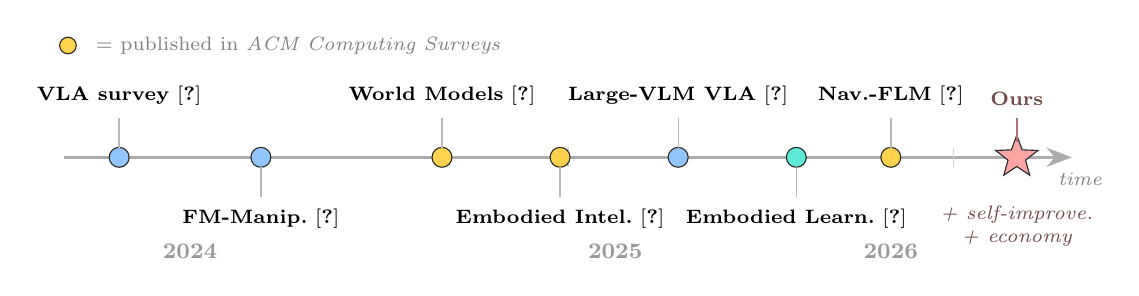
\begin{tikzpicture}[
 abv/.style={font=\scriptsize, anchor=south, align=center},
 blw/.style={font=\scriptsize, anchor=north, align=center},
 stem/.style={gray!55, line width=0.5pt},
]
 %
 \draw[-{Stealth[length=3.2mm]}, line width=1.3pt, gray!65] (-0.4,0) -- (12.4,0);
 \node[font=\scriptsize\itshape, gray, anchor=west] at (12.1,-0.28) {time};
 %
 \foreach \x in {0.3,6,10.9}{\draw[gray!35] (\x,-0.12) -- (\x,0.12);}
 \node[font=\footnotesize\bfseries,gray!80] at (1.2,-1.2) {2024};
 \node[font=\footnotesize\bfseries,gray!80] at (6.6,-1.2) {2025};
 \node[font=\footnotesize\bfseries,gray!80] at (10.1,-1.2) {2026};
 %
 \filldraw[fill=secD,draw=hidden-draw] (-0.35,1.42) circle (3pt);
 \node[font=\scriptsize,gray,anchor=west] at (-0.12,1.42) {= published in \emph{ACM Computing Surveys}};

 %
 \filldraw[fill=secA,draw=hidden-draw] (0.3,0) circle (3.6pt);
 \draw[stem] (0.3,0.12) -- (0.3,0.5); \node[abv] at (0.3,0.53) {\textbf{VLA survey}~\cite{survey_vla}};

 \filldraw[fill=secA,draw=hidden-draw] (2.1,0) circle (3.6pt);
 \draw[stem] (2.1,-0.12) -- (2.1,-0.5); \node[blw] at (2.1,-0.53) {\textbf{FM-Manip.}~\cite{survey_fmrobot}};

 \filldraw[fill=secD,draw=hidden-draw] (4.4,0) circle (3.6pt);
 \draw[stem] (4.4,0.12) -- (4.4,0.5); \node[abv] at (4.4,0.53) {\textbf{World Models}~\cite{survey_worldmodels}};

 \filldraw[fill=secD,draw=hidden-draw] (5.9,0) circle (3.6pt);
 \draw[stem] (5.9,-0.12) -- (5.9,-0.5); \node[blw] at (5.9,-0.53) {\textbf{Embodied Intel.}~\cite{survey_embodiedintel}};

 \filldraw[fill=secA,draw=hidden-draw] (7.4,0) circle (3.6pt);
 \draw[stem] (7.4,0.12) -- (7.4,0.5); \node[abv] at (7.4,0.53) {\textbf{Large-VLM VLA}~\cite{survey_vlmvla}};

 \filldraw[fill=secB,draw=hidden-draw] (8.9,0) circle (3.6pt);
 \draw[stem] (8.9,-0.12) -- (8.9,-0.5); \node[blw] at (8.9,-0.53) {\textbf{Embodied Learn.}~\cite{survey_embodiedlearn}};

 \filldraw[fill=secD,draw=hidden-draw] (10.1,0) circle (3.6pt);
 \draw[stem] (10.1,0.12) -- (10.1,0.5); \node[abv] at (10.1,0.53) {\textbf{Nav.-FLM}~\cite{survey_navigation}};

 %
 \node[star,star points=5,star point ratio=2.4,fill=secE,draw=hidden-draw,minimum size=16pt,inner sep=0] at (11.7,0) {};
 \draw[secE!70!black,line width=0.6pt] (11.7,0.2) -- (11.7,0.5);
 \node[abv,text=secE!45!black] at (11.7,0.53) {\textbf{Ours}};
 \node[blw,text=secE!45!black,font=\scriptsize\itshape] at (11.7,-0.5) {+ self-improve.\\+ economy};
\end{tikzpicture}}
\caption{The closest related surveys as a timeline (2024--2026);
\textcolor{secD!55!black}{amber} markers denote surveys published in \emph{ACM Computing
Surveys} (CSUR). Prior surveys cover VLA models, foundation models, world models, and navigation,
but none organises code-as-policy by \emph{degree of self-improvement}. \textbf{Ours}
($\star$, 2026) is organised around the self-improvement axis (\S3.1.5) and the skill economy;
per-topic coverage is in Table~\ref{tab:survey_compare}.}
\Description{A horizontal timeline of related surveys from 2024 to 2026, with amber markers for surveys
published in ACM Computing Surveys and other markers for arXiv surveys covering vision-language-action
models, foundation models, world models, and navigation; a red star at 2026 marks the present survey.}
\label{fig:surveys}
\end{figure}
 \FloatBarrier
 %
\section{A Taxonomy of Robot-Learning Techniques}
\label{sec:taxonomy}

Figure~\ref{fig:taxonomy_main} organises the field into six branches. The dividing
question is \emph{what ships}: frozen weights (\S\ref{sec:vla}) or executable skills
(\S\ref{sec:code}). We tag mechanisms by \textbf{F}eedback, \textbf{S}earch, and
\textbf{M}emory throughout.

Table~\ref{tab:compare_main} compares all systems in the map on what each \emph{ships}, where
it is evaluated, and whether it improves from its own experience.
%
%
{\footnotesize
\begin{longtable}{@{}p{0.30\textwidth}cll c c@{}}
\caption{Detailed comparison of a representative 47 of the 77 systems in the taxonomy
(Figure~\ref{fig:taxonomy_main}), grouped by family; the \S3.1 and \S3.4 branches are tabulated in
full in Tables~\ref{tab:compare_31} and~\ref{tab:compare_34}. \textbf{Ships}: \tcode/\tweights/\treward/\tskill/\tpolicy/\tbench.
\textbf{Eval}: \dreal/\dsim/\dgame. \textbf{Self-impr.}: \yy\ learns from its own experience,
\pp\ partially, \nn\ no, \dm\ n/a.}\label{tab:compare_main}\\
\toprule
\textbf{System} & \textbf{Year} & \textbf{Venue} & \textbf{Ships} & \textbf{Eval} & \textbf{Self-impr.}\\
\midrule
\endfirsthead
\multicolumn{6}{@{}l}{\footnotesize\emph{Table~\ref{tab:compare_main} (continued)}}\\
\toprule
\textbf{System} & \textbf{Year} & \textbf{Venue} & \textbf{Ships} & \textbf{Eval} & \textbf{Self-impr.}\\
\midrule
\endhead
\bottomrule
\endlastfoot
\multicolumn{6}{@{}l}{\textbf{\S3.1 Code-as-policy for robots} \hfill \tcode}\\
\textbf{Code-as-Policies}~\cite{codeaspolicies} & 2023 & ICRA & \tcode & \dreal & \nn\\
\textbf{ProgPrompt}~\cite{progprompt} & 2023 & ICRA & \tcode & \dreal & \nn\\
\textbf{VoxPoser}~\cite{voxposer} & 2023 & CoRL & \tcode & \dreal & \nn\\
\textbf{RoboCodeX}~\cite{robocodex} & 2024 & ICML & \tcode & \dsim & \nn\\
\textbf{Instruct2Act}~\cite{instruct2act} & 2023 & arXiv & \tcode & \dsim & \nn\\
\textbf{RoboPro}~\cite{robopro} & 2025 & arXiv & \tcode & \dreal & \nn\\
\textbf{RoboCoder}~\cite{robocoder} & 2024 & arXiv & \tcode & \dsim & \nn\\
\textbf{CaP-X}~\cite{capx} & 2026 & arXiv & \tcode & \dsim & \yy\\
\textbf{RoboClaw}~\cite{roboclaw} & 2026 & arXiv & \tcode & \dreal & \yy\\
\textbf{ASPIRE}~\cite{aspire} & 2026 & arXiv & \tcode & \dreal & \yy\\
\textbf{ENPIRE}~\cite{enpire} & 2026 & arXiv & \tcode & \dreal & \yy\\
\midrule
\multicolumn{6}{@{}l}{\textbf{\S3.2 End-to-end VLA / generalist policies} \hfill \tweights}\\
\textbf{RT-1}~\cite{rt1} & 2023 & RSS & \tweights & \dreal & \nn\\
\textbf{RT-2}~\cite{rt2} & 2023 & CoRL & \tweights & \dreal & \nn\\
\textbf{Octo}~\cite{octo} & 2024 & RSS & \tweights & \dreal & \nn\\
\textbf{OpenVLA}~\cite{openvla} & 2024 & CoRL & \tweights & \dreal & \nn\\
\textbf{RoboFlamingo}~\cite{roboflamingo} & 2024 & ICLR & \tweights & \dsim & \nn\\
\textbf{CogACT}~\cite{cogact} & 2024 & arXiv & \tweights & \dreal & \nn\\
\textbf{SpatialVLA}~\cite{spatialvla} & 2025 & arXiv & \tweights & \dreal & \nn\\
$\boldsymbol{\pi_0}$~\cite{pi0} & 2024 & arXiv & \tweights & \dreal & \nn\\
$\boldsymbol{\pi_{0.5}}$~\cite{pi05} & 2025 & arXiv & \tweights & \dreal & \nn\\
\textbf{GR00T N1}~\cite{groot} & 2025 & arXiv & \tweights & \dreal & \nn\\
\textbf{Gemini Robotics}~\cite{geminirobotics} & 2025 & arXiv & \tweights & \dreal & \nn\\
\midrule
\multicolumn{6}{@{}l}{\textbf{\S3.3 LLM-authored rewards / curricula} \hfill \treward}\\
\textbf{Eureka}~\cite{eureka} & 2024 & ICLR & \treward & \dsim & \yy\\
\textbf{DrEureka}~\cite{dreureka} & 2024 & RSS & \treward & \dreal & \yy\\
\textbf{Text2Reward}~\cite{text2reward} & 2024 & ICLR & \treward & \dsim & \pp\\
\textbf{Language-to-Rewards}~\cite{l2r} & 2023 & CoRL & \treward & \dreal & \pp\\
\textbf{Eurekaverse}~\cite{eurekaverse} & 2024 & CoRL & \treward & \dsim & \yy\\
\textbf{RoboGen}~\cite{robogen} & 2024 & ICML & \treward & \dsim & \yy\\
\textbf{Auto MC-Reward}~\cite{automcreward} & 2024 & CVPR & \treward & \dgame & \yy\\
\midrule
\multicolumn{6}{@{}l}{\textbf{\S3.4 Robot skill libraries \& lifelong learning} \hfill \tskill}\\
\textbf{Voyager}~\cite{voyager} & 2023 & arXiv & \tskill & \dgame & \yy\\
\textbf{LOTUS}~\cite{lotus} & 2024 & ICRA & \tskill & \dsim & \yy\\
\textbf{LRLL}~\cite{lrll} & 2024 & ICRA & \tskill & \dsim & \yy\\
\textbf{BOSS}~\cite{boss} & 2023 & CoRL & \tskill & \dsim & \yy\\
\textbf{SPRINT}~\cite{sprint} & 2024 & ICRA & \tskill & \dsim & \pp\\
\textbf{Uni-Skill}~\cite{uniskill} & 2026 & ICRA & \tskill & \dreal & \yy\\
\textbf{SkillFlow}~\cite{skillflow} & 2026 & arXiv & \tskill & \dtext & \yy\\
\midrule
\multicolumn{6}{@{}l}{\textbf{\S3.5 Sim-to-real \& cross-embodiment transfer} \hfill \tpolicy}\\
\textbf{Open X-Embodiment}~\cite{openx} & 2024 & ICRA & \tpolicy & \dreal & \nn\\
\textbf{CrossFormer}~\cite{crossformer} & 2024 & CoRL & \tpolicy & \dreal & \nn\\
\textbf{RoboCat}~\cite{robocat} & 2023 & TMLR & \tpolicy & \dreal & \yy\\
\textbf{Mirage}~\cite{mirage} & 2024 & RSS & \tpolicy & \dreal & \nn\\
\midrule
\multicolumn{6}{@{}l}{\textbf{\S3.6 Embodied benchmarks \& simulators} \hfill \tbench}\\
\textbf{LIBERO}~\cite{libero} & 2023 & NeurIPS & \tbench & \dsim & \dm\\
\textbf{Robosuite}~\cite{robosuite} & 2020 & arXiv & \tbench & \dsim & \dm\\
\textbf{BEHAVIOR-1K}~\cite{behavior1k} & 2024 & arXiv & \tbench & \dsim & \dm\\
\textbf{Meta-World}~\cite{metaworld} & 2019 & CoRL & \tbench & \dsim & \dm\\
\textbf{RLBench}~\cite{rlbench} & 2020 & RA-L & \tbench & \dsim & \dm\\
\textbf{ManiSkill2}~\cite{maniskill2} & 2023 & ICLR & \tbench & \dsim & \dm\\
\textbf{CALVIN}~\cite{calvin} & 2022 & RA-L & \tbench & \dsim & \dm\\
\end{longtable}
}
 
\subsection{Survey methodology: how the corpus was built}
\label{sec:method}

Figure~\ref{fig:prisma} summarises the corpus construction in the PRISMA~2020
style~\citep{prisma2020}. The corpus was assembled in two passes over a January~2016 to
July~2026 window. First, the 77 taxonomy systems were curated by \emph{seeding and
snowballing}: for each of the six branches we started from its landmark systems and chased
citations forward and backward until new candidates stopped appearing. Second, the 225-work
landscape corpus (Table~\ref{tab:landscape}) was gathered by five \emph{structured web-search
sweeps}, one per area cluster: (i) generalist and vision-language-action policies, imitation
and diffusion policies; (ii) language-model planning, task-and-motion planning, reward and data
synthesis; (iii) skill discovery, hierarchical reinforcement learning, and world models;
(iv) manipulation, dexterity, sim-to-real, locomotion, and benchmarks; and (v) representation
learning, offline reinforcement learning, navigation, and tactile sensing. Each sweep queried
the open web with area-specific search strings of the form ``\emph{<system or family name>
robot learning arXiv}'' and ``\emph{<area> survey/benchmark/dataset}'' over arXiv, the ACM
Digital Library, IEEE Xplore, Google Scholar, and venue proceedings pages (CoRL, RSS, ICRA,
IROS, NeurIPS, ICML, ICLR, CVPR).

\emph{Inclusion} required a work to (a) concern how an embodied agent's skill or policy is
authored, learned, transferred, evaluated, or distributed, and (b) carry verifiable metadata:
exact title, first author, year, and an arXiv identifier or DOI, each confirmed against the
source. \emph{Exclusion} removed pure perception, navigation, and locomotion work with no
bearing on skill authoring (retained only in the landscape appendix where it anchors an area),
works whose metadata could not be verified, and duplicates, detected by both bibliographic key
and arXiv identifier. Every reference in this survey passed the verification step; candidates
that failed it were discarded at harvest time, and we report that their count was not logged
rather than estimate it. Included systems were then mapped onto the taxonomy of
Figure~\ref{fig:taxonomy_main} by the mechanism definitions of Table~\ref{tab:defs}.

%
%
%
%
%
%
\begin{figure}[t]
\centering
\resizebox{\textwidth}{!}{%
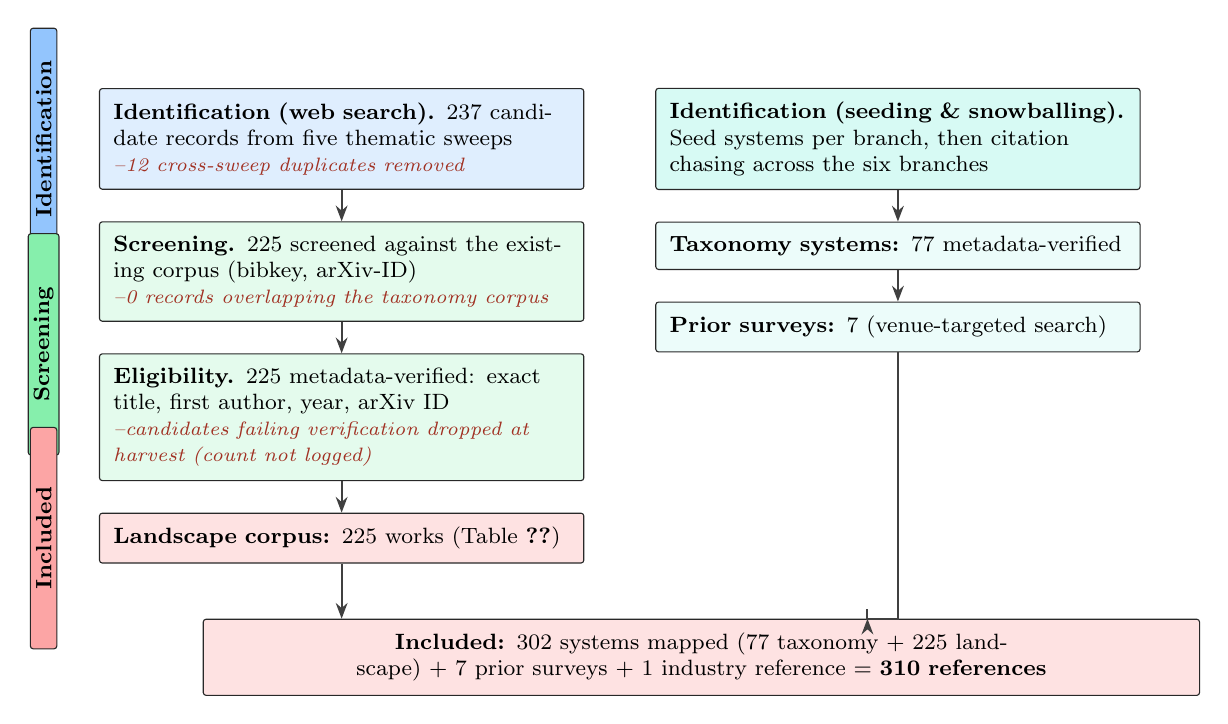
\begin{tikzpicture}[
  font=\footnotesize,
  box/.style={draw=hidden-draw, rounded corners=1pt, align=left, inner sep=5pt,
              text width=16.5em, fill=white},
  ex/.style={font=\scriptsize\itshape, text=BrickRed!85!black},
  bar/.style={draw=hidden-draw, rounded corners=1pt, inner sep=2pt, rotate=90,
              anchor=center, align=center, font=\footnotesize\bfseries, minimum width=8em},
  ar/.style={-{Stealth[length=2mm]}, darkgray, line width=0.7pt},
  node distance=4mm and 9mm,
]
%
\node[box, fill=secA!30] (L1)
  {\textbf{Identification (web search).} 237 candidate records from five thematic sweeps\\
   {\scriptsize\itshape\color{BrickRed!85!black} --12 cross-sweep duplicates removed}};
\node[box, fill=secC!22, below=of L1] (L2)
  {\textbf{Screening.} 225 screened against the existing corpus (bibkey, arXiv-ID)\\
   {\scriptsize\itshape\color{BrickRed!85!black} --0 records overlapping the taxonomy corpus}};
\node[box, fill=secC!22, below=of L2] (L3)
  {\textbf{Eligibility.} 225 metadata-verified: exact title, first author, year, arXiv ID\\
   {\scriptsize\itshape\color{BrickRed!85!black} --candidates failing verification dropped at harvest (count not logged)}};
\node[box, fill=secEl, below=of L3] (L4)
  {\textbf{Landscape corpus:} 225 works (Table~\ref{tab:landscape})};
%
\node[box, fill=secB!25, right=9mm of L1] (R1)
  {\textbf{Identification (seeding \& snowballing).} Seed systems per branch, then citation
   chasing across the six branches};
\node[box, fill=secB!12, below=of R1] (R2)
  {\textbf{Taxonomy systems:} 77 metadata-verified};
\node[box, fill=secB!12, below=of R2] (R3)
  {\textbf{Prior surveys:} 7 (venue-targeted search)};
%
\node[box, fill=secEl, below=7mm of L4, xshift=13em, text width=35em, align=center] (INC)
  {\textbf{Included:} 302 systems mapped (77 taxonomy $+$ 225 landscape) $+$ 7 prior surveys
   $+$ 1 industry reference $=$ \textbf{310 references}};
%
\draw[ar] (L1) -- (L2); \draw[ar] (L2) -- (L3); \draw[ar] (L3) -- (L4);
\draw[ar] (R1) -- (R2); \draw[ar] (R2) -- (R3);
\draw[ar] (L4.south) -- (L4.south |- INC.north);
\draw[ar] (R3.south) |- ([xshift=6em]INC.north) -- ([xshift=6em]INC.north |- INC.north);
%
\node[bar, fill=secA] at ($(L1.west)+(-2em,0)$) {Identification};
\node[bar, fill=secC] at ($(L2.west)!0.5!(L3.west)+(-2em,0)$) {Screening};
\node[bar, fill=secE] at ($(L4.west)+(-2em,0)$) {Included};
\end{tikzpicture}}
\caption{\textbf{Corpus construction} in the PRISMA 2020 style~\citep{prisma2020}. The left column
is the web-search stream behind the landscape corpus (Table~\ref{tab:landscape}), with recorded
counts and inline exclusions (red) at each stage; the right column is the seed-and-snowball
curation behind the taxonomy corpus (Figure~\ref{fig:taxonomy_main}). Both streams feed the
included set. Candidates whose metadata could not be verified were discarded at harvest time; their
count was not logged, which we state rather than estimate (\S\ref{sec:method}).}
\Description{A PRISMA 2020 style flow diagram with two identification columns. The left column
(structured web search) shows 237 candidate records, minus 12 duplicates, screened to 225 with zero
taxonomy overlap, and 225 metadata-verified records forming the landscape corpus; exclusions are
noted inline, including a note that candidates failing verification were dropped with their count
not logged. The right column (seed-and-snowball curation) yields 77 taxonomy systems and 7 prior
surveys. Both columns feed an included box of 302 systems and 310 total references. Side bars mark
the Identification, Screening, and Included stages.}
\label{fig:prisma}
\end{figure}
  %
\section{The Technique Families}
\label{sec:techniques}

We now examine each of the six branches of the taxonomy (Figure~\ref{fig:taxonomy_main}) in
turn. We begin with the code-as-policy camp (\S\ref{sec:code}), the focus of this survey and
the only family we organise by \emph{degree of self-improvement}, and then survey the
weights-based (\S\ref{sec:vla}), reward-synthesis (\S\ref{sec:reward}), skill-library
(\S\ref{sec:skill}), transfer (\S\ref{sec:transfer}), and benchmark (\S\ref{sec:bench})
families that surround it.
 %
\subsection{Code-as-Policy: Robots that Write their Own Skills}
\label{sec:code}

The organising contribution of this survey is to arrange code-as-policy methods not by
application or robot embodiment, but by \emph{how much of their own competence a system
produces at run time}. Concretely, we ask five questions in sequence: does the agent (i)
write control code at all, (ii) repair that code from execution feedback within a task,
(iii) remember validated code across tasks, (iv) search a population of programs rather
than following a single trajectory of repairs, and (v) close all of these into one
open-ended loop? Each ``yes'' is a rung on the ladder shown in the \S3.1 branch of
Figure~\ref{fig:taxonomy_main}, and
the population thins sharply toward the top: of the thirteen zero-shot systems, only a
handful ever reach the combined feedback, memory, and search regime. The purpose of this
arrangement is to name the progression and to make explicit how sparsely the top rung is
populated. We use the operational definitions of Table~\ref{tab:defs} throughout: a system
exhibits feedback, memory, or search only under the conditions stated there.

%
%
\begin{table*}[t]
\centering
\footnotesize
\renewcommand{\arraystretch}{1.3}
\begin{tabular}{@{}l p{0.42\textwidth} p{0.30\textwidth}@{}}
\toprule
\textbf{Mechanism} & \textbf{Counts (a system has it if and only if\ldots)} & \textbf{Does not count} \\
\midrule
\textbf{Feedback (F)} &
an execution-grounded signal is read and used to revise the code \emph{within} a task: a
failure detector firing, a sensory or textual summary of what went wrong, or a verifier or
reward obtained by running the program (a simulated reward qualifies when the agent uses it to
revise) &
a fresh human instruction; a fixed pre-trained value function that is never queried at run
time; a natural-language critique that is not grounded in execution \\
\textbf{Memory (M)} &
content written \emph{at run time} is stored across task boundaries and retrieved for later
tasks: a persistent code-skill library, or a retrievable episodic-text memory of past
solutions &
the model's frozen pre-trained weights; a within-task scratchpad discarded at episode end; a
fixed API library the agent cannot extend \\
\textbf{Search (S)} &
more than one candidate program is maintained, scored by execution, and selected or mutated
among: sampled-program selection, evolutionary mutation, or beam search &
a single sequential chain of repairs on one candidate (that is Feedback); one-shot sampling
with no selection; repeated prompting whose candidates are never compared \\
\bottomrule
\end{tabular}
\caption{Operational definitions of the three mechanisms used to place a system on the
code-as-policy ladder (\S\ref{sec:code}). These resolve the ambiguous boundary cases: a
failure detector or a grounded critique counts as Feedback, trained weights do not count as
Memory, and repeated prompting counts as Search only when its candidates are compared and
selected.}
\label{tab:defs}
\end{table*}
 
%
%
\begin{figure}[t]
\centering
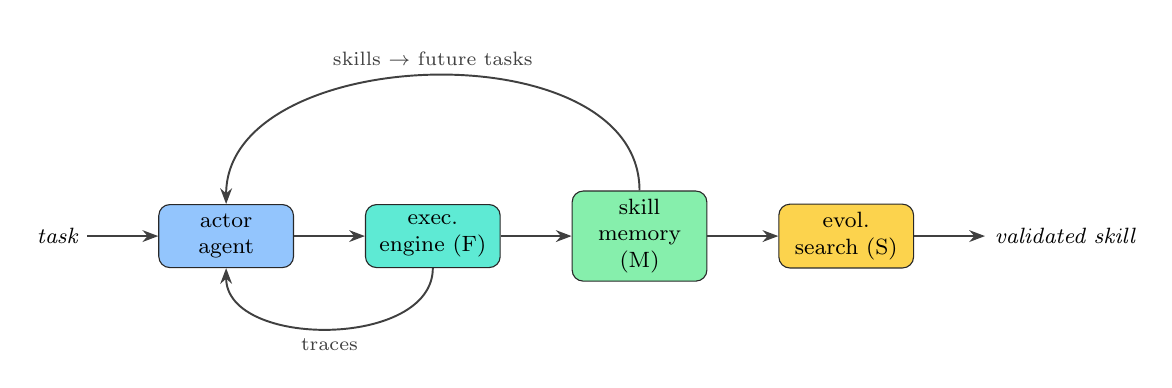
\begin{tikzpicture}[
 node distance=6mm and 9mm,
 box/.style={draw=hidden-draw, rounded corners, fill=secAl, align=center,
 font=\footnotesize, minimum height=8mm, text width=15mm, inner sep=3pt},
 core/.style={box, fill=secA},
 io/.style={draw=none, font=\footnotesize\itshape},
 ar/.style={-{Stealth[length=2mm]}, darkgray, line width=0.7pt},
]
 \node[io] (task) {task};
 \node[box, fill=secA, right=of task] (actor) {actor\\ agent};
 \node[box, fill=secB, right=of actor] (eng) {exec.\\ engine (F)};
 \node[box, fill=secC, right=of eng] (mem) {skill\\ memory (M)};
 \node[box, fill=secD, right=of mem] (srch) {evol.\\ search (S)};
 \node[io, right=of srch] (out) {validated skill};

 \draw[ar] (task) -- (actor);
 \draw[ar] (actor) -- (eng);
 \draw[ar] (eng) -- (mem);
 \draw[ar] (mem) -- (srch);
 \draw[ar] (srch) -- (out);
 %
 \draw[ar] (eng.south) to[out=-90,in=-90] node[below,font=\scriptsize]{traces} (actor.south);
 \draw[ar] (mem.north) to[out=90,in=90] node[above,font=\scriptsize]{skills $\rightarrow$ future tasks} (actor.north);
\end{tikzpicture}
\caption{The full self-improving loop (\S3.1.5): feedback (F) $+$ memory (M) $+$ search (S)
combine into one open-ended loop (occupied by ASPIRE, ENPIRE, and RoboClaw). VLAs (\S3.2) have no such loop.}
\Description{A left-to-right pipeline of five boxes: task, actor agent, execution engine (feedback),
skill memory, and evolutionary search, producing a validated skill; two return arrows feed execution
traces back to the actor and store learned skills for future tasks, forming a closed self-improving loop.}
\label{fig:architectures}
\end{figure}
 
\subsubsection{Zero-shot synthesis}
\label{ssec:zeroshot}
\emph{Membership condition:} a system is on this rung if and only if it emits executable control
code but closes no execution loop back to code generation, so feedback, memory, and search are
all absent. The foundational move is to treat the language model as a \emph{program synthesiser} over
a fixed library of perception and control primitives. \emph{Code-as-Policies}
\citep{codeaspolicies} showed that an LLM prompted with an API and a natural-language
instruction can emit executable Python that composes those primitives, recursively
defining undefined functions and parameterising control with arithmetic and feedback
logic. \emph{ProgPrompt} \citep{progprompt} situates the generated program in the scene
by exposing available actions and objects as importable symbols, while \emph{VoxPoser}
\citep{voxposer} has the model write code that \emph{composes 3D value maps} for a motion
planner rather than calling fixed skills, loosening the dependence on a hand-authored API.
Subsequent work broadened the input modality and task horizon; \emph{RoboCodeX}
\citep{robocodex} conditions on multimodal observations, \emph{Instruct2Act}
\citep{instruct2act} maps instructions to perception--action code, and video- and
demonstration-conditioned variants such as \emph{RoboPro} \citep{robopro},
\emph{Demo2Code} \citep{demo2code} and \emph{Text2Motion} \citep{text2motion} recover
programs from richer context. \emph{Statler} \citep{statler} maintains an explicit world
state across steps, and \emph{TidyBot} \citep{tidybot} and \emph{ChatGPT for Robotics}
\citep{chatgptrobotics} demonstrate personalisation and prompt design for real hardware.
What unites this rung, and limits it, is that the program is written \emph{once}: there is
no channel from execution back to the synthesiser, so a plan that fails at run time simply
fails.

\subsubsection{Closed-loop self-repair}
\label{ssec:selfrepair}
\emph{Membership condition:} feedback is present but memory and search are absent; the agent
revises code within a task from an execution-grounded signal yet retains nothing across tasks
and never compares a population of candidates. The second rung adds a within-task feedback loop. \emph{Inner Monologue}
\citep{innermonologue} feeds success detectors, scene descriptions and human feedback back
into the model as language, letting it replan when a step fails. \emph{DoReMi}
\citep{doremi} detects misalignments between plan and execution and triggers recovery, and
\emph{REFLECT} \citep{reflect} builds a hierarchical, multimodal summary of past
interaction that an LLM queries to explain a failure and propose a correction. More recent
systems push the monitor into the perception loop; \emph{Code-as-Monitor}
\citep{codeasmonitor} compiles spatio-temporal constraints into vision-language checks, and
\emph{AHA} \citep{aha} trains a model to reason explicitly about failure modes. The novelty
of this rung is the closed loop, but it is a \emph{short} loop: corrections are discarded
at task boundaries, so nothing accumulates.

\subsubsection{Skill-library accumulation}
\label{ssec:skilllib}
\emph{Membership condition:} memory is present; validated code is written to a cross-task store
and retrieved later, independently of whether within-task feedback is used. The third rung makes the loop persistent by writing validated code into a growing library
that later tasks retrieve and compose. Because this ``memory'' axis is a full technique
family in its own right, we catalogue its systems once, in \S\ref{sec:skill}
(\S3.4.3); \emph{Voyager} \citep{voyager} is the canonical example, curating an
ever-growing library of verified skill programs with when-to-apply guards, while related
methods distil language corrections into retrievable knowledge for future tasks~\citep{droc}. The key
distinction from \S3.1.2 is temporal scope: competence compounds \emph{across} tasks rather
than being rebuilt each time.

\subsubsection{Evolutionary program search}
\label{ssec:search}
\emph{Membership condition:} search is present; the agent maintains and selects among more than
one candidate program rather than repairing a single one. The fourth rung replaces a single chain of repairs with population-based search over
programs. Rather than iteratively debugging one candidate, the agent maintains several,
scores them by execution, and mutates the best. \emph{CaP-X} \citep{capx} provides an
interactive gym and benchmark for exactly this style of coding agent, and \emph{RoboEvolve}
\citep{roboevolve} couples a planner and a learned simulator into a co-evolutionary loop
that mines near-miss failures to stabilise search. The novelty is the shift from
\emph{repair} to \emph{search}: exploration is explicit and parallel, which trades compute
for a better chance of escaping local failures.

\subsubsection{The full self-improving loop}
\label{ssec:fullloop}
\emph{Membership condition:} all three mechanisms are present in one closed loop, so the rung
is the conjunction feedback \emph{and} memory \emph{and} search (Figure~\ref{fig:architectures}).
Only a few very recent systems satisfy it. \emph{ASPIRE} \citep{aspire} pairs a robot execution
engine that emits per-primitive multimodal traces with a skill library of validated code and a
population search over candidate programs; \emph{ENPIRE} \citep{enpire} closes an analogous loop
on physical hardware through automatic reset, parallel rollouts, and log-driven revision; and
\emph{RoboClaw} \citep{roboclaw} unifies data collection, policy learning, and execution under a
single controller with self-resetting loops. That this cell is so sparsely populated, rather
than any particular system within it, is the structural observation the survey is organised to
make.

Table~\ref{tab:compare_31} makes the funnel explicit, tabulating each system's use of
feedback (F), memory (M), and search (S).
%
%
{\footnotesize
\begin{longtable}{@{}p{0.36\textwidth}c ccc c@{}}
\caption{The 30 systems on the code-as-policy self-improvement ladder: the 27 of the \S3.1 branch of
Figure~\ref{fig:taxonomy_main} plus the three \S3.4.3 skill-library systems (Voyager, LRLL, Uni-Skill)
that also occupy its memory rung, on the three
self-improvement mechanisms, \textbf{F}eedback, \textbf{M}emory, \textbf{S}earch, which are
determined by the rung. \yy\ present, \nn\ absent. \textbf{Self-impr.}: \yy\ full loop,
\pp\ partial, \nn\ none.}\label{tab:compare_31}\\
\toprule
\textbf{System} & \textbf{Year} & \textbf{F} & \textbf{M} & \textbf{S} & \textbf{Self-impr.}\\
\midrule
\endfirsthead
\multicolumn{6}{@{}l}{\footnotesize\emph{Table~\ref{tab:compare_31} (continued)}}\\
\toprule
\textbf{System} & \textbf{Year} & \textbf{F} & \textbf{M} & \textbf{S} & \textbf{Self-impr.}\\
\midrule
\endhead
\bottomrule
\endlastfoot
\multicolumn{6}{@{}l}{\textbf{\S3.1.1 Zero-shot synthesis} \hfill F\,\nn\ \ M\,\nn\ \ S\,\nn}\\
\textbf{Code-as-Policies}~\cite{codeaspolicies} & 2023 & \nn & \nn & \nn & \nn\\
\textbf{ProgPrompt}~\cite{progprompt} & 2023 & \nn & \nn & \nn & \nn\\
\textbf{VoxPoser}~\cite{voxposer} & 2023 & \nn & \nn & \nn & \nn\\
\textbf{Instruct2Act}~\cite{instruct2act} & 2023 & \nn & \nn & \nn & \nn\\
\textbf{ChatGPT for Robotics}~\cite{chatgptrobotics} & 2023 & \nn & \nn & \nn & \nn\\
\textbf{TidyBot}~\cite{tidybot} & 2023 & \nn & \nn & \nn & \nn\\
\textbf{RoboCodeX}~\cite{robocodex} & 2024 & \nn & \nn & \nn & \nn\\
\textbf{RoboScript}~\cite{roboscript} & 2024 & \nn & \nn & \nn & \nn\\
\textbf{Text2Motion}~\cite{text2motion} & 2023 & \nn & \nn & \nn & \nn\\
\textbf{Demo2Code}~\cite{demo2code} & 2023 & \nn & \nn & \nn & \nn\\
\textbf{Statler}~\cite{statler} & 2024 & \nn & \nn & \nn & \nn\\
\textbf{Prompt2Walk}~\cite{prompt2walk} & 2024 & \nn & \nn & \nn & \nn\\
\textbf{RoboPro}~\cite{robopro} & 2025 & \nn & \nn & \nn & \nn\\
\midrule
\multicolumn{6}{@{}l}{\textbf{\S3.1.2 Closed-loop self-repair} \hfill F\,\yy\ \ M\,\nn\ \ S\,\nn}\\
\textbf{Inner Monologue}~\cite{innermonologue} & 2022 & \yy & \nn & \nn & \nn\\
\textbf{DoReMi}~\cite{doremi} & 2024 & \yy & \nn & \nn & \nn\\
\textbf{REFLECT}~\cite{reflect} & 2023 & \yy & \nn & \nn & \nn\\
\textbf{Code-as-Monitor}~\cite{codeasmonitor} & 2025 & \yy & \nn & \nn & \nn\\
\textbf{AHA}~\cite{aha} & 2024 & \yy & \nn & \nn & \nn\\
\textbf{Introspective Planning}~\cite{introspective} & 2024 & \yy & \nn & \nn & \nn\\
\midrule
\multicolumn{6}{@{}l}{\textbf{\S3.1.3 Skill-library accumulation} \hfill F\,\nn\ \ M\,\yy\ \ S\,\nn}\\
\textbf{Voyager}~\cite{voyager} & 2023 & \nn & \yy & \nn & \pp\\
\textbf{LRLL}~\cite{lrll} & 2024 & \nn & \yy & \nn & \pp\\
\textbf{RoboCoder}~\cite{robocoder} & 2024 & \nn & \yy & \nn & \pp\\
\textbf{Uni-Skill}~\cite{uniskill} & 2026 & \nn & \yy & \nn & \pp\\
\textbf{DROC}~\cite{droc} & 2024 & \yy & \yy & \nn & \pp\\
\midrule
\multicolumn{6}{@{}l}{\textbf{\S3.1.4 Evolutionary program search} \hfill F\,\yy\ \ M\,\nn\ \ S\,\yy}\\
\textbf{CaP-X}~\cite{capx} & 2026 & \yy & \nn & \yy & \pp\\
\textbf{RoboEvolve}~\cite{roboevolve} & 2026 & \yy & \nn & \yy & \pp\\
\textbf{Code Evolution (GEAR)}~\cite{codeevolution} & 2026 & \yy & \nn & \yy & \pp\\
\midrule
\multicolumn{6}{@{}l}{\textbf{\S3.1.5 Full self-improving loop} \hfill F\,\yy\ \ M\,\yy\ \ S\,\yy}\\
\textbf{ASPIRE}~\cite{aspire} & 2026 & \yy & \yy & \yy & \yy\\
\textbf{ENPIRE}~\cite{enpire} & 2026 & \yy & \yy & \yy & \yy\\
\textbf{RoboClaw}~\cite{roboclaw} & 2026 & \yy & \yy & \yy & \yy\\
\end{longtable}
}
  %
\subsection{End-to-End Vision-Language-Action Models}
\label{sec:vla}

The dominant alternative to writing code is to regress actions directly from pixels and
language with a single large network, so that competence lives in \emph{frozen weights}
rather than in an inspectable program. Architecturally these vision-language-action (VLA)
models share a backbone--action-head decomposition: a vision-language backbone encodes the
scene and instruction, and a pluggable action head maps that representation to motor
commands~\citep{openvla,pi0}.

The lineage begins with \emph{RT-1}~\citep{rt1}, a transformer trained on large-scale real
robot data that discretises continuous actions into categorical bins. \emph{RT-2}~\citep{rt2}
then co-fine-tunes an Internet-pretrained vision-language model on robot trajectories,
emitting actions as text tokens and inheriting semantic generalisation from web data. Open
reproductions followed: \emph{Octo}~\citep{octo} and \emph{OpenVLA}~\citep{openvla}, the
latter a 7B model with a DINOv2/SigLIP vision stack, are trained on the pooled
Open X-Embodiment corpus (\S\ref{sec:transfer}), and \emph{RoboFlamingo}~\citep{roboflamingo}
adapts a vision-language model into an imitation policy.

A second design axis is the \emph{action representation}. Discrete token heads (RT-1/RT-2)
are simple but coarse; recent systems favour continuous heads. \emph{$\pi_0$}~\citep{pi0}
attaches a \emph{flow-matching} head to a PaLI-Gemma backbone for smooth, high-frequency
bimanual control, and \emph{$\pi_{0.5}$}~\citep{pi05} extends it toward open-world
generalisation; \emph{CogACT}~\citep{cogact} separates a cognition module from a
diffusion-transformer action module, and \emph{SpatialVLA}~\citep{spatialvla} injects 3D
spatial encodings. Flow- and diffusion-based heads trade a few extra parameters for far fewer
inference steps and better high-degree-of-freedom precision.

At the largest scale, foundation-model efforts target whole platforms:
\emph{GR00T~N1}~\citep{groot} pairs a slow System-2 vision-language reasoner with a fast
System-1 diffusion transformer that produces motor actions at high rate for humanoids, and
\emph{Gemini Robotics}~\citep{geminirobotics} builds a VLA together with an embodied-reasoning
model on the Gemini backbone. Across all of these, the defining property, and the reason we
treat them as the \emph{foil} for this survey, is that there is \emph{no loop and no code}:
competence is acquired by scaling data and parameters, generalises by interpolation rather
than search, and cannot be edited, audited, or recombined after training.
 %
\subsection{Reward and Curriculum Synthesis}
\label{sec:reward}

A third family keeps the language model in the role of programmer but points it at a
different artefact: instead of policy code, it writes the \emph{reward}, \emph{environment},
or \emph{curriculum} that a reinforcement-learning loop then compiles into a policy. A
feedback loop exists, the model reads back training statistics and revises, but what ships
is still weights, which is why we separate this family from the self-improving code camp
(\S\ref{sec:code}).

\emph{Eureka}~\citep{eureka} is the canonical instance: given unmodified environment source
code and a task description, a coding LLM zero-shot generates an executable reward function,
then improves it by \emph{evolutionary search} guided by \emph{reward reflection}, a textual
summary of training statistics, exceeding expert human rewards on 83\% of a 29-task IsaacGym
suite. \emph{DrEureka}~\citep{dreureka} extends the idea to sim-to-real by also synthesising
domain-randomisation ranges, achieving zero-shot real-world locomotion.
\emph{Text2Reward}~\citep{text2reward} generates dense reward programs grounded in a compact
environment representation and refines them from human feedback, matching or beating
expert-written rewards on most of a seventeen-task suite, while \emph{Language to
Rewards}~\citep{l2r} uses the reward function as the interface between an LLM and a MuJoCo
model-predictive controller.

Beyond the reward itself, the same generative recipe is applied to the \emph{training
environment}. \emph{Eurekaverse}~\citep{eurekaverse} has an LLM propose a progressively harder
curriculum of environments, learning parkour skills that transfer to a real robot, and
\emph{RoboGen}~\citep{robogen} runs a propose-generate-learn cycle that fabricates tasks,
scenes, and supervision in simulation to unlock effectively unlimited training data;
\emph{Auto MC-Reward}~\citep{automcreward} automates dense rewards for open-world Minecraft.
The through-line is that language becomes a bridge from high-level intent to low-level control
\emph{via} an RL optimiser, rather than producing an executable, reusable skill directly.
 %
\subsection{Skill Libraries: How a Repertoire is Built}
\label{sec:skill}

Where \S\ref{sec:code} asked \emph{how} a code skill improves, this family asks the prior
question of \emph{how a repertoire of skills is built at all}. The \S3.4 branch of
Figure~\ref{fig:taxonomy_main} organises these systems along one axis, skills learned as latent reinforcement-learning policies
versus skills stored as retrievable code, and only the code flavour self-improves without
gradients, which links this family back to \S\ref{sec:code}.

Before surveying these systems we note that the word ``skill'' is badly overloaded.
Table~\ref{tab:skill_senses} separates five senses that the literature routinely conflates,
from a latent policy to a market product, and records which properties each sense affords.

%
%
\begin{table*}[t]
\centering
\footnotesize
\renewcommand{\arraystretch}{1.25}
\begin{tabular}{@{}p{0.16\textwidth} p{0.22\textwidth} p{0.18\textwidth} c c c c@{}}
\toprule
\textbf{Sense of ``skill''} & \textbf{Representation} & \textbf{Examples} &
\textbf{Inspect.} & \textbf{Adapt.} & \textbf{Compos.} & \textbf{Distrib.} \\
\midrule
latent policy & latent-conditioned network $\pi(a\mid s,z)$ & DIAYN, DADS, METRA & \nn & \pp & \nn & \nn \\
option / primitive & temporally-extended sub-policy with a skill prior & SPiRL, OPAL, SkiMo & \pp & \pp & \yy & \nn \\
code & executable program over an API & Code-as-Policies, Voyager & \yy & \yy & \yy & \pp \\
robot app & packaged, one-tap deployable behaviour & UniStore motion packages & \nn & \nn & \nn & \yy \\
market product & a listed, versioned, priced commodity & UniStore listings & \nn & \nn & \pp & \yy \\
\bottomrule
\end{tabular}
\caption{The word ``skill'' spans at least five senses that the literature frequently
conflates. Columns record whether a skill is human-\textbf{inspect}able, \textbf{adapt}able
after creation, symbolically \textbf{compos}able, and \textbf{distrib}utable across robots
(\yy\ yes, \pp\ partial, \nn\ no). Only the \emph{code} sense is inspectable, adaptable, and
composable at once; only the app and market senses are readily distributable, which is the
mismatch the skill economy (\S\ref{sec:open}) must close.}
\label{tab:skill_senses}
\end{table*}
 
\subsubsection{Unsupervised and latent skill discovery}
The oldest lineage learns a diverse set of skills with \emph{no task reward and no code}, by
maximising an information-theoretic objective. \emph{DIAYN}~\citep{diayn} maximises the mutual
information between a latent skill code and the visited states, yielding distinguishable
behaviours; \emph{DADS}~\citep{dads} makes the discovered skills dynamics-aware and hence
usable for model-based control; and \emph{LSD}~\citep{lsd}, \emph{CIC}~\citep{cic}, and
\emph{METRA}~\citep{metra} push toward more dynamic, far-reaching, and scalable skills through
Lipschitz constraints, contrastive objectives, and metric-aware abstractions respectively.

\subsubsection{Skill-based and hierarchical reinforcement learning}
A second lineage extracts a continuous \emph{skill space} from offline data and then plans or
learns within it. \emph{SPiRL}~\citep{spirl} learns a skill embedding together with a skill
prior that accelerates downstream RL; \emph{OPAL}~\citep{opal} discovers temporally extended
primitives for offline RL; \emph{PARROT}~\citep{parrot} learns an invertible behavioural
prior; and \emph{SkiMo}~\citep{skimo} learns a skill dynamics model so that planning happens
directly in skill space.

\subsubsection{LLM and code skill libraries}
The code flavour, where the self-improving methods of \S\ref{sec:code} live, stores skills as
retrievable programs. \emph{Voyager}~\citep{voyager} curates an ever-growing library of
verified code skills in Minecraft; \emph{LOTUS}~\citep{lotus} performs continual imitation
learning through unsupervised skill discovery; \emph{LRLL}~\citep{lrll} bootstraps a composable
robot library with language models; and \emph{BOSS}~\citep{boss} and \emph{SPRINT}~\citep{sprint}
grow skill repertoires by LLM-guided bootstrapping and instruction relabelling. The most recent
entries close the loop between video and code: \emph{Uni-Skill}~\citep{uniskill} builds a
self-evolving skill repository from unstructured robot video, and \emph{SkillFlow}~\citep{skillflow}
benchmarks lifelong discovery, patching, and reuse of a skill library.

\subsubsection{Open-world LLM-agent libraries}
Finally, embodied LLM agents accumulate skills from open-ended experience.
\emph{GITM}~\citep{gitm} and \emph{JARVIS-1}~\citep{jarvis1} pair a planner with text or
multimodal memory in Minecraft; \emph{ExpeL}~\citep{expel} extracts reusable insights from a
stream of trials; \emph{Optimus-1}~\citep{optimus1} adds a hybrid multimodal memory for
long-horizon tasks; and \emph{Odyssey}~\citep{odyssey} equips an agent with an open-world
library of primitive and compositional skills. These systems foreshadow the marketplace
dynamics of \S\ref{sec:open}: a library that grows with use.

Table~\ref{tab:compare_34} contrasts the four sub-families on skill form, whether they are
gradient-trained or LLM-authored, whether they keep a persistent library, and their domain.
%
%
{\footnotesize
\begin{longtable}{@{}p{0.30\textwidth}c l c c c@{}}
\caption{The 21 skill-building systems of the \S3.4 branch of Figure~\ref{fig:taxonomy_main}, by sub-family.
\textbf{Form}: \flatent/\fspace/\fcodelib/\fagent. \textbf{Grad.}: gradient-trained (\yy) vs
LLM-authored (\nn). \textbf{Lib.}: persistent retrievable library. \textbf{Domain}:
\dsim/\dgame/\dreal/\dtext.}\label{tab:compare_34}\\
\toprule
\textbf{System} & \textbf{Year} & \textbf{Form} & \textbf{Grad.} & \textbf{Lib.} & \textbf{Domain}\\
\midrule
\endfirsthead
\multicolumn{6}{@{}l}{\footnotesize\emph{Table~\ref{tab:compare_34} (continued)}}\\
\toprule
\textbf{System} & \textbf{Year} & \textbf{Form} & \textbf{Grad.} & \textbf{Lib.} & \textbf{Domain}\\
\midrule
\endhead
\bottomrule
\endlastfoot
\multicolumn{6}{@{}l}{\textbf{\S3.4.1 Unsupervised / latent discovery (RL)}}\\
\textbf{DIAYN}~\cite{diayn} & 2019 & \flatent & \yy & \nn & \dsim\\
\textbf{DADS}~\cite{dads} & 2020 & \flatent & \yy & \nn & \dsim\\
\textbf{LSD}~\cite{lsd} & 2022 & \flatent & \yy & \nn & \dsim\\
\textbf{CIC}~\cite{cic} & 2022 & \flatent & \yy & \nn & \dsim\\
\textbf{METRA}~\cite{metra} & 2024 & \flatent & \yy & \nn & \dsim\\
\midrule
\multicolumn{6}{@{}l}{\textbf{\S3.4.2 Skill-based / hierarchical RL}}\\
\textbf{SPiRL}~\cite{spirl} & 2020 & \fspace & \yy & \nn & \dsim\\
\textbf{OPAL}~\cite{opal} & 2021 & \fspace & \yy & \nn & \dsim\\
\textbf{PARROT}~\cite{parrot} & 2021 & \fspace & \yy & \nn & \dsim\\
\textbf{SkiMo}~\cite{skimo} & 2022 & \fspace & \yy & \nn & \dsim\\
\midrule
\multicolumn{6}{@{}l}{\textbf{\S3.4.3 LLM / code skill libraries}}\\
\textbf{Voyager}~\cite{voyager} & 2023 & \fcodelib & \nn & \yy & \dgame\\
\textbf{LOTUS}~\cite{lotus} & 2024 & \fcodelib & \nn & \yy & \dsim\\
\textbf{LRLL}~\cite{lrll} & 2024 & \fcodelib & \nn & \yy & \dsim\\
\textbf{BOSS}~\cite{boss} & 2023 & \fcodelib & \nn & \yy & \dsim\\
\textbf{SPRINT}~\cite{sprint} & 2024 & \fcodelib & \nn & \yy & \dsim\\
\textbf{Uni-Skill}~\cite{uniskill} & 2026 & \fcodelib & \nn & \yy & \dreal\\
\textbf{SkillFlow}~\cite{skillflow} & 2026 & \fcodelib & \nn & \yy & \dtext\\
\midrule
\multicolumn{6}{@{}l}{\textbf{\S3.4.4 Open-world LLM-agent libraries}}\\
\textbf{GITM}~\cite{gitm} & 2023 & \fagent & \nn & \yy & \dgame\\
\textbf{JARVIS-1}~\cite{jarvis1} & 2023 & \fagent & \nn & \yy & \dgame\\
\textbf{ExpeL}~\cite{expel} & 2024 & \fagent & \nn & \yy & \dtext\\
\textbf{Optimus-1}~\cite{optimus1} & 2024 & \fagent & \nn & \yy & \dgame\\
\textbf{Odyssey}~\cite{odyssey} & 2024 & \fagent & \nn & \yy & \dgame\\
\end{longtable}
}
  %
\subsection{Sim-to-Real and Cross-Embodiment Transfer}
\label{sec:transfer}

A skill is only useful if it moves across the simulation-to-reality gap and across robot
bodies. The enabling artefact is scale: \emph{Open X-Embodiment}~\citep{openx} pools sixty
datasets from twenty-one institutions into over a million trajectories spanning twenty-two
embodiments and hundreds of skills, and shows that RT-X models trained on the mixture exhibit
positive transfer and emergent capabilities across platforms.

Given such data, a single network can control very different bodies.
\emph{CrossFormer}~\citep{crossformer} trains one transformer on 900K trajectories across
twenty embodiments, arms, wheeled robots, quadrotors, and quadrupeds, \emph{without} manually
aligning observation or action spaces, and matches specialist policies tailored to each robot.
Other work attacks transfer at test time rather than through data:
\emph{Mirage}~\citep{mirage} achieves \emph{zero-shot} cross-embodiment transfer by
``cross-painting'', masking the target robot and inpainting the source robot at the same pose
so the policy sees a familiar body, and bridging the control gap with forward dynamics.

The most suggestive point for this survey is \emph{RoboCat}~\citep{robocat}, a goal-conditioned
multi-embodiment agent that adapts to a new task from as few as a hundred demonstrations and
then \emph{generates its own data} for the next training round, forming a rudimentary
self-improvement loop of the kind \S\ref{sec:code} makes explicit. This is also the marketplace
question of \S\ref{sec:open}: a skill advertised for the G1, H1, B2, and Go2
platforms must survive exactly the cross-embodiment gap these methods study.
 %
\subsection{Benchmarks and Evaluation}
\label{sec:bench}

Progress in the families above is measured on a shared set of simulated benchmarks, most of
which report a single-number success rate. \emph{LIBERO}~\citep{libero} targets lifelong
manipulation and knowledge transfer across task suites; \emph{Meta-World}~\citep{metaworld}
offers fifty manipulation tasks for multi-task and meta-reinforcement learning;
\emph{RLBench}~\citep{rlbench} provides a hundred vision-based tasks with demonstrations; and
\emph{ManiSkill2}~\citep{maniskill2} adds GPU-parallel simulation over twenty task families.
\emph{Robosuite}~\citep{robosuite} is the modular MuJoCo framework underlying many of these,
and \emph{CALVIN}~\citep{calvin} evaluates long-horizon, language-conditioned control by the
average number of sub-tasks completed in a chain. At the high-realism end,
\emph{BEHAVIOR-1K}~\citep{behavior1k} specifies a thousand everyday household activities in a
photorealistic simulator, scoring both success and efficiency.

Table~\ref{tab:matrix} contrasts one exemplar per camp on the axes that separate them. The
recurring gap, and a direct motivation for the open problems of \S\ref{sec:open}, is that
these suites measure \emph{one-shot competence}: they report whether a policy succeeds, not
whether it \emph{improves with experience}. No standard benchmark yet plots held-out success as
a function of accumulated interaction, which is exactly the quantity the self-improvement ladder
of \S\ref{sec:code} is designed to raise.

%
%
\begin{table*}[t]
\centering
\footnotesize
\renewcommand{\arraystretch}{1.25}
\begin{tabular}{@{}p{0.25\textwidth}cccc@{}}
\toprule
\textbf{Dimension}
 & \textcolor{cat-code!50!black}{\textbf{Full loop}}~\cite{aspire,enpire,roboclaw}
 & \textbf{$\pi_0$}~\cite{pi0}
 & \textbf{Code-as-Pol.}~\cite{codeaspolicies}
 & \textbf{Eureka}~\cite{eureka} \\
 & {\footnotesize\itshape code+skills} & {\footnotesize\itshape VLA weights}
 & {\footnotesize\itshape code, no mem.} & {\footnotesize\itshape reward} \\
\midrule
What it outputs & skill code+lib & action chunks & policy code & reward code \\
How it improves & F+M+S loop & gradient pretrain & \dm\,one-shot & RL+reflection \\
Gradient training? & \nn & \yy & \nn & \yy \\
Persistent skill library? & \yy & \nn & \nn & \nn \\
Failure feedback signal & exec.\ traces & \dm & \dm & train.\ stats \\
Search strategy & evolutionary & \dm & \dm & \dm \\
Real-robot validation & \yy & \yy & \yy & \yy \\
Continual / open-ended? & \yy & \nn & \nn & \nn \\
Beyond fixed APIs? & \yy & \yy & \nn & \dm \\
Interpretable / editable? & \yy & \nn & \yy & \yy \\
\bottomrule
\end{tabular}
\caption{Capability matrix, one representative per camp. Only the full-loop cell (\S3.1.5; e.g.\ ASPIRE,
ENPIRE, RoboClaw) combines a persistent skill library with feedback- and search-driven
self-improvement; each other camp lacks at least one axis. \yy~= yes, \nn~= no, \dm~= n/a.}
\label{tab:matrix}
\end{table*}
 
\subsection{Synthesis: what each family cannot do}
\label{sec:synthesis}
Table~\ref{tab:branch_limits} compares every family on six axes: data needs, task horizon,
transfer, interpretability, safety, and characteristic failure mode. Reading it column-wise
profiles a family; reading it row-wise shows that every axis has at least one weak family, and
no family is favourable on all six, which is the tension the skill economy (\S\ref{sec:open})
inherits.

%
%
%
\begin{table*}[t]
\centering
\scriptsize
\setlength{\tabcolsep}{3pt}
\renewcommand{\arraystretch}{1.45}
\begin{tabular}{@{}>{\raggedright\arraybackslash}p{0.125\textwidth} >{\raggedright\arraybackslash}p{0.16\textwidth} >{\raggedright\arraybackslash}p{0.16\textwidth} >{\raggedright\arraybackslash}p{0.15\textwidth} >{\raggedright\arraybackslash}p{0.15\textwidth} >{\raggedright\arraybackslash}p{0.155\textwidth}@{}}
\toprule
 & \textbf{End-to-end VLA} (\S\ref{sec:vla}) & \textbf{Code-as-policy} (\S\ref{sec:code})
 & \textbf{Reward synthesis} (\S\ref{sec:reward}) & \textbf{RL skill discovery} (\S\ref{sec:skill})
 & \textbf{Market skills} (\S\ref{sec:open}) \\
\midrule
\textbf{Data needs} &
\nn\ web-scale teleop corpora: 1M+ episodes, 22 embodiments~\citep{openx} &
\yy\ few-shot prompts over a pretrained LLM~\citep{codeaspolicies} &
\pp\ massive \emph{simulated} interaction, no demonstrations~\citep{eureka} &
\nn\ millions of environment steps per embodiment~\citep{diayn} &
\yy\ none at deployment; vendor-recorded playback~\citep{unistore2026} \\
\textbf{Task horizon} &
\pp\ short reactive chunks; long tasks by chaining~\citep{rt2} &
\yy\ long: programs compose perception and control primitives~\citep{voxposer} &
\nn\ one low-level skill per synthesised reward~\citep{eureka} &
\nn\ temporally-extended primitives, not full tasks~\citep{metra} &
\pp\ fixed multi-step routines; no branching \\
\textbf{Transfer} &
\yy\ cross-task and cross-embodiment via co-training~\citep{openx} &
\pp\ API-level portability, but bound to the perception stack &
\pp\ sim-to-real via randomisation search~\citep{dreureka} &
\pp\ latent skills seed downstream RL~\citep{spirl} &
\nn\ certified robot models only; no adaptation~\citep{unistore2026} \\
\textbf{Interpretability} &
\nn\ opaque weights; behaviour only observable &
\yy\ readable, editable, diffable programs &
\pp\ readable reward code; opaque trained policy &
\nn\ latent skill codes, symbolically uninspectable &
\nn\ sealed vendor package \\
\textbf{Safety} &
\nn\ emergent behaviour is hard to verify pre-deployment &
\yy\ inspectable before execution; constrained to vetted APIs &
\nn\ reward hacking; unintended optima~\citep{eureka} &
\nn\ unconstrained exploration unsafe on hardware &
\pp\ vendor certification, but no provenance record \\
\textbf{Failure mode} &
silent misgrounding under distribution shift &
brittle when perception mislabels the scene &
specification gaming that passes in sim only &
skill collapse into degenerate behaviours &
context mismatch with no recovery path \\
\bottomrule
\end{tabular}
\caption{\textbf{Family comparison matrix}: the five technique families on six axes (data needs,
task horizon, transfer, interpretability, safety, characteristic failure mode). Marks grade each
family on the axis (\yy\ favourable, \pp\ mixed, \nn\ weak); evidence anchors include the
Open X-Embodiment corpus~\citep{openx} for data and transfer and lifelong suites such as
LIBERO~\citep{libero} for horizon and reuse. No family is favourable on all six axes, which is
the tension the skill economy (\S\ref{sec:open}) inherits.}
\label{tab:branch_limits}
\end{table*}
  %
\section{The Skill Economy: Open Problems}
\label{sec:open}

The arrival of a commercial marketplace for robot skills (Unitree's UniStore ships
one-tap, cross-model motion packages~\citep{unistore2026}) turns several research
questions from hypothetical into pressing. We frame them as the open agenda of this survey.

\paragraph{The static-to-adaptive gap.}
Every skill shipped today is, in effect, replayed: a motion package or a fixed program is
installed and executed without perceiving whether \emph{this} kitchen, gripper, or object
differs from the one it was authored for. The techniques of \S\ref{sec:code}, within-task
repair, persistent memory, and search, are precisely what would let a downloaded skill
\emph{adapt} on the target robot. Closing this gap is the difference between a store of
animations and a store of capabilities, and it is the direct application of the \S3.1.5
loop to a distribution setting where the base skill is given rather than discovered.

\paragraph{Cross-embodiment portability.}
UniStore advertises a single skill running across the G1 and H1 humanoids and the B2/Go2
quadrupeds; bodies with different morphologies, action spaces, and dynamics. This is the
cross-embodiment transfer problem (\S\ref{sec:transfer}) at deployment scale: without a
shared action interface \citep{openx} or explicit embodiment adaptation, a package tuned
for one platform has no guarantee of correctness on another. Formal portability, what must
hold for a skill to be certified on a new body, remains open.

\paragraph{Provenance and trust.}
A marketplace invites third-party, crowdsourced uploads, including raw motion-capture data
and code from unknown authors. Robot skills act on the physical world, so provenance
(who authored a skill, from what data, validated how) becomes a safety property, not merely
a metadata nicety. There is no accepted standard for signing, attesting, or auditing a
robot skill's origin.

\paragraph{Safety verification.}
Vendors promise that ``every skill is scanned, tested, and verified,'' but for a
code-as-policy skill this is undecidable in general and hard in practice: the skill's effect
depends on the scene it meets. Practical questions include which pre-conditions a skill must
declare, what sandboxed or simulated screening it must pass, and how run-time monitors
(cf.\ \emph{Code-as-Monitor} \citep{codeasmonitor}) can bound behaviour on unseen inputs.

\paragraph{Skill composition.}
Downloading two skills should ideally yield a third: ``make coffee'' plus ``clear the
table'' composed into a morning routine. Composition requires shared interfaces and a
calculus over pre-/post-conditions; today's motion packages are opaque and do not compose,
and code skills compose only within a single authoring system.

\paragraph{Portability standards and skill ontologies.}
Reuse at scale needs a shared vocabulary: declared pre-conditions, expected effects, and
embodiment-capability profiles, with relations such as \emph{requires}, \emph{provides}, and
\emph{substitutable-by}. Prior work on skill ontologies and hardware-level reusability
points the way, but no cross-vendor standard exists, which is what a genuine ecosystem would
require.

\paragraph{Local versus shared libraries.}
Finally, the field must reconcile two notions of ``skill library'' that this survey has kept
distinct: the \emph{self-built} library a robot grows from its own experience
(\S\ref{sec:code}) and the \emph{shared} library a robot downloads from a marketplace
(UniStore). The interesting regime is the hybrid, an agent that both contributes to and
draws from a commons, and its incentives, quality control, and feedback dynamics are
entirely unstudied.
 %
\section{Limitations of this Survey}
\label{sec:limitations}

We state the boundaries of the survey explicitly. First, our organising axis, \emph{degree
of self-improvement}, is deliberately code-centric; it foregrounds systems that emit and
revise programs and treats weight-based policies (\S\ref{sec:vla}) and reinforcement-learning
skill discovery (\S\ref{sec:skill}) as context rather than as the object of the taxonomy.
A survey centred on representation learning or on real-world data collection would draw the
map differently. Second, the frontier we emphasise (\S3.1.5) is populated by very recent,
in some cases concurrent, systems; benchmark numbers across them are not directly
comparable, and we therefore report capabilities qualitatively rather than ranking methods.
Third, the field moves quickly: several 2025--2026 systems we cite were released while this
survey was being written, and the coverage should be read as a snapshot. Finally, the
``skill economy'' framing (\S\ref{sec:open}) is grounded in an emerging commercial trend
(one vendor's marketplace at the time of writing); we treat it as motivation for open
problems, not as a mature body of results.
 %
\section{Future Directions}
\label{sec:future}

To make the agenda actionable rather than aspirational, we anchor it on four measurable
quantities, defined with concrete testbeds in Table~\ref{tab:future_metrics}: the
\emph{success-vs-interactions curve} (does competence rise with autonomous experience?), the
\emph{skill-library reuse rate} (does stored competence compound?), the \emph{cross-embodiment
transfer drop} (how much is lost when a skill changes bodies?), and the \emph{provenance check}
(can a distributed skill's origin and test record be verified?). The first two instantiate
naturally on LIBERO-style lifelong task streams~\citep{libero}; the third on held-out-embodiment
splits of Open X-Embodiment~\citep{openx}; the fourth on marketplace
listings~\citep{unistore2026}.

%
%
\begin{table*}[t]
\centering
\footnotesize
\setlength{\tabcolsep}{4pt}
\renewcommand{\arraystretch}{1.35}
\begin{tabular}{@{}p{0.17\textwidth} p{0.30\textwidth} p{0.27\textwidth} p{0.17\textwidth}@{}}
\toprule
\textbf{Metric} & \textbf{Definition} & \textbf{Instantiation (testbed)} & \textbf{Family stressed} \\
\midrule
Success-vs-interactions curve &
held-out success rate as a function of accumulated autonomous interactions; report the curve
and its area, not a single endpoint &
lifelong task streams in the style of LIBERO-100~\citep{libero}, fixed interaction budget &
\S\ref{sec:code} full loop; \S\ref{sec:vla} fine-tuning \\
Skill-library reuse rate &
fraction of new-task solutions that invoke at least one previously stored skill, and mean
invocations per stored skill &
growing code libraries~\citep{voyager} evaluated across LIBERO-style task suites~\citep{libero} &
\S\ref{sec:skill} libraries; \S\ref{sec:code} memory rung \\
Cross-embodiment transfer drop &
difference in success between the training embodiment and an unseen one, at matched task and
budget &
held-out-embodiment splits of Open X-Embodiment~\citep{openx} (22 embodiments) &
\S\ref{sec:vla}; \S\ref{sec:transfer} \\
Provenance check &
fraction of distributed skills carrying a verifiable origin, training-data statement, and
reproducible test record &
audits of marketplace listings~\citep{unistore2026} against a declared provenance schema &
market skills (\S\ref{sec:open}) \\
\bottomrule
\end{tabular}
\caption{\textbf{An actionable protocol for the future agenda}: four measurable quantities, their
definitions, and concrete testbeds. The first two instantiate LIBERO-style lifelong
learning~\citep{libero}; the third instantiates Open X-Embodiment-style multi-robot
transfer~\citep{openx}; the fourth targets the skill marketplaces of \S\ref{sec:open}.}
\label{tab:future_metrics}
\end{table*}
 
Three directions follow directly from the map, each now with its success measure.
\textbf{(1) Standardised evaluation of self-improvement.} The systems on the top rung
(\S3.1.5) each report improvement on their own splits; the field lacks a shared protocol that
plots the success-vs-interactions curve and the skill-library reuse rate under a common interaction
budget. A benchmark that publishes both curves per system, in the way LIBERO standardised
lifelong manipulation~\citep{libero}, would make ``self-improvement'' a reported number rather
than a claim. \textbf{(2) Adaptation as a first-class marketplace primitive.} The open problems
of \S\ref{sec:open} suggest a research programme in which a downloaded skill is not a frozen
artefact but a starting point that the \S\ref{sec:code} loop specialises to the local robot and
environment; its success measures are the transfer drop before versus after on-device
adaptation, and the provenance check on what was downloaded. \textbf{(3) Bridging the RL and
code flavours of skills.} \S\ref{sec:skill} shows that skills are learned either as latent RL
policies or as retrievable code; a unifying interface, code that wraps, calls, and refines
learned policies, and learned policies distilled back into inspectable code, would let the
self-improvement machinery of \S\ref{sec:code} operate over both, and its progress is legible in
the reuse rate crossing family boundaries. We see the combination of a standard self-improvement
benchmark with an adaptation-centric marketplace as the most likely path from today's static
skill stores to genuinely capable, compounding robots.
 %
\section{Conclusion}
\label{sec:conclusion}

Robot learning is organising itself around a single question: should competence be shipped
as \emph{weights} or as \emph{skills}? This survey took that question as its axis. We mapped
the field into six branches (\S\ref{sec:taxonomy}), positioned end-to-end vision-language-
action models as the weights-based foil (\S\ref{sec:vla}), and gave the code-as-policy camp
its own deep-dive (\S\ref{sec:code}) organised by \emph{degree of self-improvement}: from
one-shot program synthesis, through within-task repair, persistent skill memory, and
population search, to the open-ended loop that combines all three. That top cell, feedback
$+$ memory $+$ search, is the least populated and least surveyed region of the field, and
it is where systems such as ASPIRE, ENPIRE, and RoboClaw now sit. We complemented this with a map of
how skill \emph{repertoires} are built (\S\ref{sec:skill}), showing that skills come in an
RL flavour and a code flavour of which only the latter self-improves without gradients, and
we connected the academic taxonomy to the nascent skill economy (\S\ref{sec:open}), where
commercial marketplaces already distribute skills but ship only static playback. The gap
between that static distribution and genuine on-device adaptation is, we argue, the defining
research opportunity for physical AI, and the self-improvement ladder of \S\ref{sec:code} offers a structured path toward closing it.
 
\bibliographystyle{ACM-Reference-Format}
%
%
%
%

\begin{thebibliography}{311}

%
%
%
%
%
%
%
%
%
%
%
%
%
%
%
%

\ifx \showCODEN    \undefined \def \showCODEN     #1{\unskip}     \fi
\ifx \showDOI      \undefined \def \showDOI       #1{#1}\fi
\ifx \showISBNx    \undefined \def \showISBNx     #1{\unskip}     \fi
\ifx \showISBNxiii \undefined \def \showISBNxiii  #1{\unskip}     \fi
\ifx \showISSN     \undefined \def \showISSN      #1{\unskip}     \fi
\ifx \showLCCN     \undefined \def \showLCCN      #1{\unskip}     \fi
\ifx \shownote     \undefined \def \shownote      #1{#1}          \fi
\ifx \showarticletitle \undefined \def \showarticletitle #1{#1}   \fi
\ifx \showURL      \undefined \def \showURL       {\relax}        \fi
%
%
\providecommand\bibfield[2]{#2}
\providecommand\bibinfo[2]{#2}
\providecommand\natexlab[1]{#1}
\providecommand\showeprint[2][]{arXiv:#2}

\bibitem[Achiam et~al\mbox{.}(2018)]%
        {valor}
\bibfield{author}{\bibinfo{person}{Joshua Achiam}, \bibinfo{person}{Harrison
  Edwards}, \bibinfo{person}{Dario Amodei}, {and} \bibinfo{person}{Pieter
  Abbeel}.} \bibinfo{year}{2018}\natexlab{}.
\newblock \showarticletitle{Variational Option Discovery Algorithms}.
\newblock \bibinfo{journal}{\emph{arXiv preprint arXiv:1807.10299}}
  (\bibinfo{year}{2018}).
\newblock


\bibitem[Adeniji et~al\mbox{.}(2023)]%
        {lamp}
\bibfield{author}{\bibinfo{person}{Ademi Adeniji}, \bibinfo{person}{Amber Xie},
  \bibinfo{person}{Carmelo Sferrazza}, \bibinfo{person}{Younggyo Seo},
  \bibinfo{person}{Stephen James}, {and} \bibinfo{person}{Pieter Abbeel}.}
  \bibinfo{year}{2023}\natexlab{}.
\newblock \showarticletitle{Language Reward Modulation for Pretraining
  Reinforcement Learning}.
\newblock \bibinfo{journal}{\emph{arXiv preprint arXiv:2308.12270}}
  (\bibinfo{year}{2023}).
\newblock


\bibitem[Agarwal et~al\mbox{.}(2022)]%
        {egoloco}
\bibfield{author}{\bibinfo{person}{Ananye Agarwal}, \bibinfo{person}{Ashish
  Kumar}, \bibinfo{person}{Jitendra Malik}, {and} \bibinfo{person}{Deepak
  Pathak}.} \bibinfo{year}{2022}\natexlab{}.
\newblock \showarticletitle{Legged Locomotion in Challenging Terrains using
  Egocentric Vision}. In \bibinfo{booktitle}{\emph{Conference on Robot Learning
  (CoRL)}}.
\newblock
\newblock
\shownote{arXiv:2211.07638}.


\bibitem[Ahn et~al\mbox{.}(2022)]%
        {saycan}
\bibfield{author}{\bibinfo{person}{Michael Ahn}, \bibinfo{person}{Anthony
  Brohan}, \bibinfo{person}{Noah Brown}, \bibinfo{person}{Yevgen Chebotar},
  \bibinfo{person}{Omar Cortes}, {et~al\mbox{.}}}
  \bibinfo{year}{2022}\natexlab{}.
\newblock \showarticletitle{Do As I Can, Not As I Say: Grounding Language in
  Robotic Affordances}.
\newblock \bibinfo{journal}{\emph{arXiv preprint arXiv:2204.01691}}
  (\bibinfo{year}{2022}).
\newblock


\bibitem[Ajay et~al\mbox{.}(2023)]%
        {decisiondiffuser}
\bibfield{author}{\bibinfo{person}{Anurag Ajay} {et~al\mbox{.}}}
  \bibinfo{year}{2023}\natexlab{}.
\newblock \showarticletitle{Is Conditional Generative Modeling all you need for
  Decision-Making?}. In \bibinfo{booktitle}{\emph{International Conference on
  Learning Representations (ICLR)}}.
\newblock
\newblock
\shownote{arXiv:2211.15657}.


\bibitem[Ajay et~al\mbox{.}(2021)]%
        {opal}
\bibfield{author}{\bibinfo{person}{Anurag Ajay}, \bibinfo{person}{Aviral
  Kumar}, \bibinfo{person}{Pulkit Agrawal}, \bibinfo{person}{Sergey Levine},
  {and} \bibinfo{person}{Ofir Nachum}.} \bibinfo{year}{2021}\natexlab{}.
\newblock \showarticletitle{OPAL: Offline Primitive Discovery for Accelerating
  Offline Reinforcement Learning}. In \bibinfo{booktitle}{\emph{International
  Conference on Learning Representations (ICLR)}}.
\newblock
\newblock
\shownote{arXiv:2010.13611}.


\bibitem[Akkaya et~al\mbox{.}(2019)]%
        {rubikscube}
\bibfield{author}{\bibinfo{person}{Ilge Akkaya} {et~al\mbox{.}}}
  \bibinfo{year}{2019}\natexlab{}.
\newblock \showarticletitle{Solving Rubik's Cube with a Robot Hand}.
\newblock \bibinfo{journal}{\emph{arXiv preprint arXiv:1910.07113}}
  (\bibinfo{year}{2019}).
\newblock


\bibitem[Alonso et~al\mbox{.}(2024)]%
        {diamond}
\bibfield{author}{\bibinfo{person}{Eloi Alonso}, \bibinfo{person}{Adam Jelley},
  \bibinfo{person}{Vincent Micheli}, \bibinfo{person}{Anssi Kanervisto},
  \bibinfo{person}{Amos Storkey}, \bibinfo{person}{Tim Pearce}, {and}
  \bibinfo{person}{Fran\c{c}ois Fleuret}.} \bibinfo{year}{2024}\natexlab{}.
\newblock \showarticletitle{Diffusion for World Modeling: Visual Details Matter
  in Atari}. In \bibinfo{booktitle}{\emph{Advances in Neural Information
  Processing Systems (NeurIPS)}}.
\newblock
\newblock
\shownote{arXiv:2405.12399}.


\bibitem[Andrychowicz et~al\mbox{.}(2018)]%
        {dactyl}
\bibfield{author}{\bibinfo{person}{Marcin Andrychowicz} {et~al\mbox{.}}}
  \bibinfo{year}{2018}\natexlab{}.
\newblock \showarticletitle{Learning Dexterous In-Hand Manipulation}.
\newblock \bibinfo{journal}{\emph{arXiv preprint arXiv:1808.00177}}
  (\bibinfo{year}{2018}).
\newblock


\bibitem[Bacon et~al\mbox{.}(2017)]%
        {optioncritic}
\bibfield{author}{\bibinfo{person}{Pierre-Luc Bacon}, \bibinfo{person}{Jean
  Harb}, {and} \bibinfo{person}{Doina Precup}.}
  \bibinfo{year}{2017}\natexlab{}.
\newblock \showarticletitle{The Option-Critic Architecture}. In
  \bibinfo{booktitle}{\emph{Proceedings of the AAAI Conference on Artificial
  Intelligence}}.
\newblock
\newblock
\shownote{arXiv:1609.05140}.


\bibitem[Bahl et~al\mbox{.}(2023)]%
        {vrb}
\bibfield{author}{\bibinfo{person}{Shikhar Bahl}, \bibinfo{person}{Russell
  Mendonca}, \bibinfo{person}{Lili Chen}, \bibinfo{person}{Unnat Jain}, {and}
  \bibinfo{person}{Deepak Pathak}.} \bibinfo{year}{2023}\natexlab{}.
\newblock \showarticletitle{Affordances from Human Videos as a Versatile
  Representation for Robotics}. In \bibinfo{booktitle}{\emph{IEEE/CVF
  Conference on Computer Vision and Pattern Recognition (CVPR)}}.
\newblock
\newblock
\shownote{arXiv:2304.08488}.


\bibitem[Bharadhwaj et~al\mbox{.}(2024)]%
        {roboagent}
\bibfield{author}{\bibinfo{person}{Homanga Bharadhwaj} {et~al\mbox{.}}}
  \bibinfo{year}{2024}\natexlab{}.
\newblock \showarticletitle{{RoboAgent}: Generalization and Efficiency in Robot
  Manipulation via Semantic Augmentations and Action Chunking}. In
  \bibinfo{booktitle}{\emph{IEEE International Conference on Robotics and
  Automation (ICRA)}}.
\newblock
\newblock
\shownote{arXiv:2309.01918}.


\bibitem[Black et~al\mbox{.}(2024b)]%
        {susie}
\bibfield{author}{\bibinfo{person}{Kevin Black} {et~al\mbox{.}}}
  \bibinfo{year}{2024}\natexlab{b}.
\newblock \showarticletitle{Zero-Shot Robotic Manipulation with Pretrained
  Image-Editing Diffusion Models}. In \bibinfo{booktitle}{\emph{International
  Conference on Learning Representations (ICLR)}}.
\newblock
\newblock
\shownote{arXiv:2310.10639}.


\bibitem[Black et~al\mbox{.}(2025)]%
        {pi05}
\bibfield{author}{\bibinfo{person}{Kevin Black}, \bibinfo{person}{Noah Brown},
  \bibinfo{person}{James Darpinian}, \bibinfo{person}{Karan Dhabalia},
  \bibinfo{person}{Danny Driess}, \bibinfo{person}{Adnan Esmail},
  \bibinfo{person}{Michael Equi}, \bibinfo{person}{Chelsea Finn},
  \bibinfo{person}{Niccolo Fusai}, \bibinfo{person}{Manuel~Y. Galliker},
  \bibinfo{person}{Dibya Ghosh}, \bibinfo{person}{Lachy Groom},
  \bibinfo{person}{Karol Hausman}, \bibinfo{person}{Brian Ichter},
  \bibinfo{person}{Szymon Jakubczak}, \bibinfo{person}{Tim Jones},
  \bibinfo{person}{Liyiming Ke}, \bibinfo{person}{Devin LeBlanc},
  \bibinfo{person}{Sergey Levine}, \bibinfo{person}{Adrian Li-Bell},
  \bibinfo{person}{Mohith Mothukuri}, \bibinfo{person}{Suraj Nair},
  \bibinfo{person}{Karl Pertsch}, \bibinfo{person}{Allen~Z. Ren},
  \bibinfo{person}{Lucy~Xiaoyang Shi}, \bibinfo{person}{Laura Smith},
  \bibinfo{person}{Jost~Tobias Springenberg}, \bibinfo{person}{Kyle
  Stachowicz}, \bibinfo{person}{James Tanner}, \bibinfo{person}{Quan Vuong},
  \bibinfo{person}{Homer Walke}, \bibinfo{person}{Anna Walling},
  \bibinfo{person}{Haohuan Wang}, \bibinfo{person}{Lili Yu}, {and}
  \bibinfo{person}{Ury Zhilinsky}.} \bibinfo{year}{2025}\natexlab{}.
\newblock \showarticletitle{{$\pi_{0.5}$}: A Vision-Language-Action Model with
  Open-World Generalization}.
\newblock \bibinfo{journal}{\emph{arXiv preprint}} (\bibinfo{year}{2025}).
\newblock
\newblock
\shownote{Physical Intelligence. arXiv:2504.16054}.


\bibitem[Black et~al\mbox{.}(2024a)]%
        {pi0}
\bibfield{author}{\bibinfo{person}{Kevin Black}, \bibinfo{person}{Noah Brown},
  \bibinfo{person}{Danny Driess}, \bibinfo{person}{Adnan Esmail},
  \bibinfo{person}{Michael Equi}, \bibinfo{person}{Chelsea Finn},
  \bibinfo{person}{Niccolo Fusai}, \bibinfo{person}{Lachy Groom},
  \bibinfo{person}{Karol Hausman}, \bibinfo{person}{Brian Ichter},
  \bibinfo{person}{Szymon Jakubczak}, \bibinfo{person}{Tim Jones},
  \bibinfo{person}{Liyiming Ke}, \bibinfo{person}{Sergey Levine},
  \bibinfo{person}{Adrian Li-Bell}, \bibinfo{person}{Mohith Mothukuri},
  \bibinfo{person}{Suraj Nair}, \bibinfo{person}{Karl Pertsch},
  \bibinfo{person}{Lucy~Xiaoyang Shi}, \bibinfo{person}{James Tanner},
  \bibinfo{person}{Quan Vuong}, \bibinfo{person}{Anna Walling},
  \bibinfo{person}{Haohuan Wang}, {and} \bibinfo{person}{Ury Zhilinsky}.}
  \bibinfo{year}{2024}\natexlab{a}.
\newblock \showarticletitle{{$\pi_0$}: A Vision-Language-Action Flow Model for
  General Robot Control}.
\newblock \bibinfo{journal}{\emph{arXiv preprint}} (\bibinfo{year}{2024}).
\newblock
\newblock
\shownote{Physical Intelligence. arXiv:2410.24164}.


\bibitem[Bousmalis et~al\mbox{.}(2023)]%
        {robocat}
\bibfield{author}{\bibinfo{person}{Konstantinos Bousmalis},
  \bibinfo{person}{Giulia Vezzani}, \bibinfo{person}{Dushyant Rao},
  \bibinfo{person}{Coline Devin}, \bibinfo{person}{Alex~X. Lee},
  \bibinfo{person}{Maria Bauza}, {et~al\mbox{.}}}
  \bibinfo{year}{2023}\natexlab{}.
\newblock \showarticletitle{RoboCat: A Self-Improving Generalist Agent for
  Robotic Manipulation}.
\newblock \bibinfo{journal}{\emph{Transactions on Machine Learning Research
  (TMLR)}} (\bibinfo{year}{2023}).
\newblock
\newblock
\shownote{arXiv:2306.11706}.


\bibitem[Brohan et~al\mbox{.}(2023a)]%
        {rt1}
\bibfield{author}{\bibinfo{person}{Anthony Brohan}, \bibinfo{person}{Noah
  Brown}, \bibinfo{person}{Justice Carbajal}, {et~al\mbox{.}}}
  \bibinfo{year}{2023}\natexlab{a}.
\newblock \showarticletitle{RT-1: Robotics Transformer for Real-World Control
  at Scale}. In \bibinfo{booktitle}{\emph{Robotics: Science and Systems
  (RSS)}}.
\newblock
\newblock
\shownote{arXiv:2212.06817}.


\bibitem[Brohan et~al\mbox{.}(2023b)]%
        {rt2}
\bibfield{author}{\bibinfo{person}{Anthony Brohan}, \bibinfo{person}{Noah
  Brown}, \bibinfo{person}{Justice Carbajal}, {et~al\mbox{.}}}
  \bibinfo{year}{2023}\natexlab{b}.
\newblock \showarticletitle{RT-2: Vision-Language-Action Models Transfer Web
  Knowledge to Robotic Control}. In \bibinfo{booktitle}{\emph{Conference on
  Robot Learning (CoRL)}}.
\newblock
\newblock
\shownote{arXiv:2307.15818}.


\bibitem[Bruce et~al\mbox{.}(2024)]%
        {genie}
\bibfield{author}{\bibinfo{person}{Jake Bruce}, \bibinfo{person}{Michael
  Dennis}, \bibinfo{person}{Ashley Edwards}, \bibinfo{person}{Jack
  Parker-Holder}, {et~al\mbox{.}}} \bibinfo{year}{2024}\natexlab{}.
\newblock \showarticletitle{Genie: Generative Interactive Environments}. In
  \bibinfo{booktitle}{\emph{International Conference on Machine Learning
  (ICML)}}.
\newblock
\newblock
\shownote{arXiv:2402.15391}.


\bibitem[Campos et~al\mbox{.}(2020)]%
        {edl}
\bibfield{author}{\bibinfo{person}{Victor Campos}, \bibinfo{person}{Alexander
  Trott}, \bibinfo{person}{Caiming Xiong}, \bibinfo{person}{Richard Socher},
  \bibinfo{person}{Xavier Giro-i Nieto}, {and} \bibinfo{person}{Jordi Torres}.}
  \bibinfo{year}{2020}\natexlab{}.
\newblock \showarticletitle{Explore, Discover and Learn: Unsupervised Discovery
  of State-Covering Skills}. In \bibinfo{booktitle}{\emph{International
  Conference on Machine Learning (ICML)}}.
\newblock
\newblock
\shownote{arXiv:2002.03647}.


\bibitem[Carta et~al\mbox{.}(2023)]%
        {glam}
\bibfield{author}{\bibinfo{person}{Thomas Carta}, \bibinfo{person}{Cl{\'e}ment
  Romac}, \bibinfo{person}{Thomas Wolf}, \bibinfo{person}{Sylvain Lamprier},
  \bibinfo{person}{Olivier Sigaud}, {and} \bibinfo{person}{Pierre-Yves
  Oudeyer}.} \bibinfo{year}{2023}\natexlab{}.
\newblock \showarticletitle{Grounding Large Language Models in Interactive
  Environments with Online Reinforcement Learning}.
\newblock \bibinfo{journal}{\emph{arXiv preprint arXiv:2302.02662}}
  (\bibinfo{year}{2023}).
\newblock


\bibitem[Cheang et~al\mbox{.}(2024)]%
        {gr2}
\bibfield{author}{\bibinfo{person}{Chi-Lam Cheang} {et~al\mbox{.}}}
  \bibinfo{year}{2024}\natexlab{}.
\newblock \showarticletitle{{GR-2}: A Generative Video-Language-Action Model
  with Web-Scale Knowledge for Robot Manipulation}.
\newblock \bibinfo{journal}{\emph{arXiv preprint arXiv:2410.06158}}
  (\bibinfo{year}{2024}).
\newblock


\bibitem[Chebotar et~al\mbox{.}(2023)]%
        {qtransformer}
\bibfield{author}{\bibinfo{person}{Yevgen Chebotar} {et~al\mbox{.}}}
  \bibinfo{year}{2023}\natexlab{}.
\newblock \showarticletitle{{Q-Transformer}: Scalable Offline Reinforcement
  Learning via Autoregressive Q-Functions}. In
  \bibinfo{booktitle}{\emph{Conference on Robot Learning (CoRL)}}.
\newblock
\newblock
\shownote{arXiv:2309.10150}.


\bibitem[Chebotar et~al\mbox{.}(2019)]%
        {simopt}
\bibfield{author}{\bibinfo{person}{Yevgen Chebotar}, \bibinfo{person}{Ankur
  Handa}, \bibinfo{person}{Viktor Makoviychuk}, \bibinfo{person}{Miles
  Macklin}, \bibinfo{person}{Jan Issac}, \bibinfo{person}{Nathan Ratliff},
  {and} \bibinfo{person}{Dieter Fox}.} \bibinfo{year}{2019}\natexlab{}.
\newblock \showarticletitle{Closing the Sim-to-Real Loop: Adapting Simulation
  Randomization with Real World Experience}. In \bibinfo{booktitle}{\emph{IEEE
  International Conference on Robotics and Automation (ICRA)}}.
\newblock
\newblock
\shownote{arXiv:1810.05687}.


\bibitem[Chen et~al\mbox{.}(2022)]%
        {transdreamer}
\bibfield{author}{\bibinfo{person}{Chang Chen}, \bibinfo{person}{Yi-Fu Wu},
  \bibinfo{person}{Jaesik Yoon}, {and} \bibinfo{person}{Sungjin Ahn}.}
  \bibinfo{year}{2022}\natexlab{}.
\newblock \showarticletitle{{TransDreamer}: Reinforcement Learning with
  Transformer World Models}.
\newblock \bibinfo{journal}{\emph{arXiv preprint arXiv:2202.09481}}
  (\bibinfo{year}{2022}).
\newblock


\bibitem[Chen et~al\mbox{.}(2026)]%
        {roboevolve}
\bibfield{author}{\bibinfo{person}{Harold~Haodong Chen}, \bibinfo{person}{Sirui
  Chen}, \bibinfo{person}{Yingjie Xu}, \bibinfo{person}{Wenhang Ge}, {and}
  \bibinfo{person}{Ying-Cong Chen}.} \bibinfo{year}{2026}\natexlab{}.
\newblock \showarticletitle{RoboEvolve: Co-Evolving Planner-Simulator for
  Robotic Manipulation with Limited Data}.
\newblock \bibinfo{journal}{\emph{arXiv preprint}} (\bibinfo{year}{2026}).
\newblock
\newblock
\shownote{arXiv:2605.13775}.


\bibitem[Chen et~al\mbox{.}(2024c)]%
        {roboscript}
\bibfield{author}{\bibinfo{person}{Junting Chen}, \bibinfo{person}{Yao Mu},
  \bibinfo{person}{Qiaojun Yu}, \bibinfo{person}{Tianming Wei},
  \bibinfo{person}{Silang Wu}, \bibinfo{person}{Zhecheng Yuan},
  \bibinfo{person}{Zhixuan Liang}, \bibinfo{person}{Chao Yang},
  \bibinfo{person}{Kaipeng Zhang}, \bibinfo{person}{Wenqi Shao},
  \bibinfo{person}{Yu Qiao}, \bibinfo{person}{Huazhe Xu},
  \bibinfo{person}{Mingyu Ding}, {and} \bibinfo{person}{Ping Luo}.}
  \bibinfo{year}{2024}\natexlab{c}.
\newblock \showarticletitle{RoboScript: Code Generation for Free-Form
  Manipulation Tasks across Real and Simulation}.
\newblock \bibinfo{journal}{\emph{arXiv preprint}} (\bibinfo{year}{2024}).
\newblock
\newblock
\shownote{arXiv:2402.14623}.


\bibitem[Chen et~al\mbox{.}(2021)]%
        {decisiontransformer}
\bibfield{author}{\bibinfo{person}{Lili Chen}, \bibinfo{person}{Kevin Lu},
  \bibinfo{person}{Aravind Rajeswaran}, \bibinfo{person}{Kimin Lee},
  \bibinfo{person}{Aditya Grover}, \bibinfo{person}{Michael Laskin},
  \bibinfo{person}{Pieter Abbeel}, \bibinfo{person}{Aravind Srinivas}, {and}
  \bibinfo{person}{Igor Mordatch}.} \bibinfo{year}{2021}\natexlab{}.
\newblock \showarticletitle{Decision Transformer: Reinforcement Learning via
  Sequence Modeling}. In \bibinfo{booktitle}{\emph{Advances in Neural
  Information Processing Systems (NeurIPS)}}.
\newblock
\newblock
\shownote{arXiv:2106.01345}.


\bibitem[Chen et~al\mbox{.}(2024a)]%
        {mirage}
\bibfield{author}{\bibinfo{person}{Lawrence~Yunliang Chen},
  \bibinfo{person}{Kush Hari}, \bibinfo{person}{Karthik Dharmarajan},
  \bibinfo{person}{Chenfeng Xu}, \bibinfo{person}{Quan Vuong}, {and}
  \bibinfo{person}{Ken Goldberg}.} \bibinfo{year}{2024}\natexlab{a}.
\newblock \showarticletitle{Mirage: Cross-Embodiment Zero-Shot Policy Transfer
  with Cross-Painting}. In \bibinfo{booktitle}{\emph{Robotics: Science and
  Systems (RSS)}}.
\newblock
\newblock
\shownote{arXiv:2402.19249}.


\bibitem[Chen et~al\mbox{.}(2023d)]%
        {visualdexterity}
\bibfield{author}{\bibinfo{person}{Tao Chen}, \bibinfo{person}{Megha Tippur},
  \bibinfo{person}{Siyang Wu}, \bibinfo{person}{Vikash Kumar},
  \bibinfo{person}{Edward Adelson}, {and} \bibinfo{person}{Pulkit Agrawal}.}
  \bibinfo{year}{2023}\natexlab{d}.
\newblock \showarticletitle{Visual Dexterity: In-Hand Reorientation of Novel
  and Complex Object Shapes}.
\newblock \bibinfo{journal}{\emph{Science Robotics}} (\bibinfo{year}{2023}).
\newblock
\newblock
\shownote{arXiv:2211.11744}.


\bibitem[Chen et~al\mbox{.}(2024b)]%
        {dgpo}
\bibfield{author}{\bibinfo{person}{Wentse Chen}, \bibinfo{person}{Shiyu Huang},
  \bibinfo{person}{Yuan Chiang}, \bibinfo{person}{Ting Chen}, {and}
  \bibinfo{person}{Jun Zhu}.} \bibinfo{year}{2024}\natexlab{b}.
\newblock \showarticletitle{{DGPO}: Discovering Multiple Strategies with
  Diversity-Guided Policy Optimization}. In
  \bibinfo{booktitle}{\emph{Proceedings of the AAAI Conference on Artificial
  Intelligence}}.
\newblock
\newblock
\shownote{arXiv:2207.05631}.


\bibitem[Chen et~al\mbox{.}(2023a)]%
        {autotamp}
\bibfield{author}{\bibinfo{person}{Yongchao Chen}, \bibinfo{person}{Jacob
  Arkin}, \bibinfo{person}{Yang Zhang}, \bibinfo{person}{Nicholas Roy}, {and}
  \bibinfo{person}{Chuchu Fan}.} \bibinfo{year}{2023}\natexlab{a}.
\newblock \showarticletitle{{AutoTAMP}: Autoregressive Task and Motion Planning
  with LLMs as Translators and Checkers}.
\newblock \bibinfo{journal}{\emph{arXiv preprint arXiv:2306.06531}}
  (\bibinfo{year}{2023}).
\newblock


\bibitem[Chen et~al\mbox{.}(2023b)]%
        {nl2tl}
\bibfield{author}{\bibinfo{person}{Yongchao Chen}, \bibinfo{person}{Rujul
  Gandhi}, \bibinfo{person}{Yang Zhang}, {and} \bibinfo{person}{Chuchu Fan}.}
  \bibinfo{year}{2023}\natexlab{b}.
\newblock \showarticletitle{{NL2TL}: Transforming Natural Languages to Temporal
  Logics using Large Language Models}.
\newblock \bibinfo{journal}{\emph{arXiv preprint arXiv:2305.07766}}
  (\bibinfo{year}{2023}).
\newblock


\bibitem[Chen et~al\mbox{.}(2023c)]%
        {genaug}
\bibfield{author}{\bibinfo{person}{Zoey Chen}, \bibinfo{person}{Sho Kiami},
  \bibinfo{person}{Abhishek Gupta}, {and} \bibinfo{person}{Vikash Kumar}.}
  \bibinfo{year}{2023}\natexlab{c}.
\newblock \showarticletitle{{GenAug}: Retargeting behaviors to unseen
  situations via Generative Augmentation}.
\newblock \bibinfo{journal}{\emph{arXiv preprint arXiv:2302.06671}}
  (\bibinfo{year}{2023}).
\newblock


\bibitem[Cheng et~al\mbox{.}(2024a)]%
        {exbody}
\bibfield{author}{\bibinfo{person}{Xuxin Cheng}, \bibinfo{person}{Yandong Ji},
  \bibinfo{person}{Junming Chen}, \bibinfo{person}{Ruihan Yang},
  \bibinfo{person}{Ge Yang}, {and} \bibinfo{person}{Xiaolong Wang}.}
  \bibinfo{year}{2024}\natexlab{a}.
\newblock \showarticletitle{Expressive Whole-Body Control for Humanoid Robots}.
  In \bibinfo{booktitle}{\emph{Robotics: Science and Systems (RSS)}}.
\newblock
\newblock
\shownote{arXiv:2402.16796}.


\bibitem[Cheng et~al\mbox{.}(2024b)]%
        {extremeparkour}
\bibfield{author}{\bibinfo{person}{Xuxin Cheng}, \bibinfo{person}{Kexin Shi},
  \bibinfo{person}{Ananye Agarwal}, {and} \bibinfo{person}{Deepak Pathak}.}
  \bibinfo{year}{2024}\natexlab{b}.
\newblock \showarticletitle{Extreme Parkour with Legged Robots}. In
  \bibinfo{booktitle}{\emph{IEEE International Conference on Robotics and
  Automation (ICRA)}}.
\newblock
\newblock
\shownote{arXiv:2309.14341}.


\bibitem[Chi et~al\mbox{.}(2023)]%
        {diffusionpolicy}
\bibfield{author}{\bibinfo{person}{Cheng Chi} {et~al\mbox{.}}}
  \bibinfo{year}{2023}\natexlab{}.
\newblock \showarticletitle{Diffusion Policy: Visuomotor Policy Learning via
  Action Diffusion}. In \bibinfo{booktitle}{\emph{Robotics: Science and Systems
  (RSS)}}.
\newblock
\newblock
\shownote{arXiv:2303.04137}.


\bibitem[Chi et~al\mbox{.}(2024)]%
        {umi}
\bibfield{author}{\bibinfo{person}{Cheng Chi} {et~al\mbox{.}}}
  \bibinfo{year}{2024}\natexlab{}.
\newblock \showarticletitle{Universal Manipulation Interface: In-The-Wild Robot
  Teaching Without In-The-Wild Robots}. In \bibinfo{booktitle}{\emph{Robotics:
  Science and Systems (RSS)}}.
\newblock
\newblock
\shownote{arXiv:2402.10329}.


\bibitem[Chua et~al\mbox{.}(2018)]%
        {pets}
\bibfield{author}{\bibinfo{person}{Kurtland Chua}, \bibinfo{person}{Roberto
  Calandra}, \bibinfo{person}{Rowan McAllister}, {and} \bibinfo{person}{Sergey
  Levine}.} \bibinfo{year}{2018}\natexlab{}.
\newblock \showarticletitle{Deep Reinforcement Learning in a Handful of Trials
  using Probabilistic Dynamics Models}. In \bibinfo{booktitle}{\emph{Advances
  in Neural Information Processing Systems (NeurIPS)}}.
\newblock
\newblock
\shownote{arXiv:1805.12114}.


\bibitem[Dasari et~al\mbox{.}(2019)]%
        {robonet}
\bibfield{author}{\bibinfo{person}{Sudeep Dasari}, \bibinfo{person}{Frederik
  Ebert}, \bibinfo{person}{Stephen Tian}, \bibinfo{person}{Suraj Nair},
  \bibinfo{person}{Bernadette Bucher}, \bibinfo{person}{Karl Schmeckpeper},
  \bibinfo{person}{Siddharth Singh}, \bibinfo{person}{Sergey Levine}, {and}
  \bibinfo{person}{Chelsea Finn}.} \bibinfo{year}{2019}\natexlab{}.
\newblock \showarticletitle{{RoboNet}: Large-Scale Multi-Robot Learning}. In
  \bibinfo{booktitle}{\emph{Conference on Robot Learning (CoRL)}}.
\newblock
\newblock
\shownote{arXiv:1910.11215}.


\bibitem[Ding et~al\mbox{.}(2025)]%
        {survey_worldmodels}
\bibfield{author}{\bibinfo{person}{Jingtao Ding} {et~al\mbox{.}}}
  \bibinfo{year}{2025}\natexlab{}.
\newblock \showarticletitle{Understanding World or Predicting Future? A
  Comprehensive Survey of World Models}.
\newblock \bibinfo{journal}{\emph{Comput. Surveys}} (\bibinfo{year}{2025}).
\newblock
\newblock
\shownote{arXiv:2411.14499}.


\bibitem[Ding et~al\mbox{.}(2022)]%
        {cowp}
\bibfield{author}{\bibinfo{person}{Yan Ding}, \bibinfo{person}{Xiaohan Zhang},
  \bibinfo{person}{Saeid Amiri}, \bibinfo{person}{Nieqing Cao},
  \bibinfo{person}{Hao Yang}, {et~al\mbox{.}}} \bibinfo{year}{2022}\natexlab{}.
\newblock \showarticletitle{Robot Task Planning and Situation Handling in Open
  Worlds}.
\newblock \bibinfo{journal}{\emph{arXiv preprint arXiv:2210.01287}}
  (\bibinfo{year}{2022}).
\newblock


\bibitem[Ding et~al\mbox{.}(2023)]%
        {llmgrop}
\bibfield{author}{\bibinfo{person}{Yan Ding}, \bibinfo{person}{Xiaohan Zhang},
  \bibinfo{person}{Chris Paxton}, {and} \bibinfo{person}{Shiqi Zhang}.}
  \bibinfo{year}{2023}\natexlab{}.
\newblock \showarticletitle{Task and Motion Planning with Large Language Models
  for Object Rearrangement}.
\newblock \bibinfo{journal}{\emph{arXiv preprint arXiv:2303.06247}}
  (\bibinfo{year}{2023}).
\newblock


\bibitem[Doshi et~al\mbox{.}(2024)]%
        {crossformer}
\bibfield{author}{\bibinfo{person}{Ria Doshi}, \bibinfo{person}{Homer Walke},
  \bibinfo{person}{Oier Mees}, \bibinfo{person}{Sudeep Dasari}, {and}
  \bibinfo{person}{Sergey Levine}.} \bibinfo{year}{2024}\natexlab{}.
\newblock \showarticletitle{Scaling Cross-Embodied Learning: One Policy for
  Manipulation, Navigation, Locomotion and Aviation}. In
  \bibinfo{booktitle}{\emph{Conference on Robot Learning (CoRL)}}.
\newblock
\newblock
\shownote{arXiv:2408.11812}.


\bibitem[Driess et~al\mbox{.}(2023)]%
        {palme}
\bibfield{author}{\bibinfo{person}{Danny Driess} {et~al\mbox{.}}}
  \bibinfo{year}{2023}\natexlab{}.
\newblock \showarticletitle{{PaLM-E}: An Embodied Multimodal Language Model}.
  In \bibinfo{booktitle}{\emph{International Conference on Machine Learning
  (ICML)}}.
\newblock
\newblock
\shownote{arXiv:2303.03378}.


\bibitem[Du et~al\mbox{.}(2023a)]%
        {unipi}
\bibfield{author}{\bibinfo{person}{Yilun Du} {et~al\mbox{.}}}
  \bibinfo{year}{2023}\natexlab{a}.
\newblock \showarticletitle{Learning Universal Policies via Text-Guided Video
  Generation}. In \bibinfo{booktitle}{\emph{Advances in Neural Information
  Processing Systems (NeurIPS)}}.
\newblock
\newblock
\shownote{arXiv:2302.00111}.


\bibitem[Du et~al\mbox{.}(2023b)]%
        {ellm}
\bibfield{author}{\bibinfo{person}{Yuqing Du}, \bibinfo{person}{Olivia
  Watkins}, \bibinfo{person}{Zihan Wang}, \bibinfo{person}{C{\'e}dric Colas},
  \bibinfo{person}{Trevor Darrell}, \bibinfo{person}{Pieter Abbeel},
  \bibinfo{person}{Abhishek Gupta}, {and} \bibinfo{person}{Jacob Andreas}.}
  \bibinfo{year}{2023}\natexlab{b}.
\newblock \showarticletitle{Guiding Pretraining in Reinforcement Learning with
  Large Language Models}.
\newblock \bibinfo{journal}{\emph{arXiv preprint arXiv:2302.06692}}
  (\bibinfo{year}{2023}).
\newblock


\bibitem[Duan et~al\mbox{.}(2024)]%
        {aha}
\bibfield{author}{\bibinfo{person}{Jiafei Duan}, \bibinfo{person}{Wilbert
  Pumacay}, \bibinfo{person}{Nishanth Kumar}, \bibinfo{person}{Yi~Ru Wang},
  \bibinfo{person}{Shulin Tian}, \bibinfo{person}{Wentao Yuan},
  \bibinfo{person}{Ranjay Krishna}, \bibinfo{person}{Dieter Fox},
  \bibinfo{person}{Ajay Mandlekar}, {and} \bibinfo{person}{Yijie Guo}.}
  \bibinfo{year}{2024}\natexlab{}.
\newblock \showarticletitle{AHA: A Vision-Language-Model for Detecting and
  Reasoning Over Failures in Robotic Manipulation}.
\newblock \bibinfo{journal}{\emph{arXiv preprint}} (\bibinfo{year}{2024}).
\newblock
\newblock
\shownote{arXiv:2410.00371}.


\bibitem[Eisner et~al\mbox{.}(2022)]%
        {flowbot3d}
\bibfield{author}{\bibinfo{person}{Ben Eisner}, \bibinfo{person}{Harry Zhang},
  {and} \bibinfo{person}{David Held}.} \bibinfo{year}{2022}\natexlab{}.
\newblock \showarticletitle{{FlowBot3D}: Learning 3D Articulation Flow to
  Manipulate Articulated Objects}. In \bibinfo{booktitle}{\emph{Robotics:
  Science and Systems (RSS)}}.
\newblock
\newblock
\shownote{arXiv:2205.04382}.


\bibitem[Eysenbach et~al\mbox{.}(2019)]%
        {diayn}
\bibfield{author}{\bibinfo{person}{Benjamin Eysenbach},
  \bibinfo{person}{Abhishek Gupta}, \bibinfo{person}{Julian Ibarz}, {and}
  \bibinfo{person}{Sergey Levine}.} \bibinfo{year}{2019}\natexlab{}.
\newblock \showarticletitle{Diversity is All You Need: Learning Skills without
  a Reward Function}. In \bibinfo{booktitle}{\emph{International Conference on
  Learning Representations (ICLR)}}.
\newblock
\newblock
\shownote{arXiv:1802.06070}.


\bibitem[Fang et~al\mbox{.}(2023a)]%
        {rh20t}
\bibfield{author}{\bibinfo{person}{Hao-Shu Fang}, \bibinfo{person}{Hongjie
  Fang}, \bibinfo{person}{Zhenyu Tang}, \bibinfo{person}{Jirong Liu},
  \bibinfo{person}{Chenxi Wang}, \bibinfo{person}{Junbo Wang},
  \bibinfo{person}{Haoyi Zhu}, {and} \bibinfo{person}{Cewu Lu}.}
  \bibinfo{year}{2023}\natexlab{a}.
\newblock \showarticletitle{{RH20T}: A Comprehensive Robotic Dataset for
  Learning Diverse Skills in One-Shot}.
\newblock \bibinfo{journal}{\emph{arXiv preprint arXiv:2307.00595}}
  (\bibinfo{year}{2023}).
\newblock


\bibitem[Fang et~al\mbox{.}(2023b)]%
        {anygrasp}
\bibfield{author}{\bibinfo{person}{Hao-Shu Fang}, \bibinfo{person}{Chenxi
  Wang}, \bibinfo{person}{Hongjie Fang}, \bibinfo{person}{Minghao Gou},
  \bibinfo{person}{Jirong Liu}, \bibinfo{person}{Hengxu Yan},
  \bibinfo{person}{Wenhai Liu}, \bibinfo{person}{Yichen Xie}, {and}
  \bibinfo{person}{Cewu Lu}.} \bibinfo{year}{2023}\natexlab{b}.
\newblock \showarticletitle{{AnyGrasp}: Robust and Efficient Grasp Perception
  in Spatial and Temporal Domains}.
\newblock \bibinfo{journal}{\emph{IEEE Transactions on Robotics (T-RO)}}
  (\bibinfo{year}{2023}).
\newblock
\newblock
\shownote{arXiv:2212.08333}.


\bibitem[Fang et~al\mbox{.}(2020)]%
        {graspnet1b}
\bibfield{author}{\bibinfo{person}{Hao-Shu Fang}, \bibinfo{person}{Chenxi
  Wang}, \bibinfo{person}{Minghao Gou}, {and} \bibinfo{person}{Cewu Lu}.}
  \bibinfo{year}{2020}\natexlab{}.
\newblock \showarticletitle{{GraspNet-1Billion}: A Large-Scale Benchmark for
  General Object Grasping}. In \bibinfo{booktitle}{\emph{IEEE/CVF Conference on
  Computer Vision and Pattern Recognition (CVPR)}}.
\newblock
\newblock
\shownote{doi:10.1109/CVPR42600.2020.01146}.


\bibitem[Florence et~al\mbox{.}(2021)]%
        {ibc}
\bibfield{author}{\bibinfo{person}{Pete Florence} {et~al\mbox{.}}}
  \bibinfo{year}{2021}\natexlab{}.
\newblock \showarticletitle{Implicit Behavioral Cloning}. In
  \bibinfo{booktitle}{\emph{Conference on Robot Learning (CoRL)}}.
\newblock
\newblock
\shownote{arXiv:2109.00137}.


\bibitem[Florensa et~al\mbox{.}(2017)]%
        {snn4hrl}
\bibfield{author}{\bibinfo{person}{Carlos Florensa}, \bibinfo{person}{Yan
  Duan}, {and} \bibinfo{person}{Pieter Abbeel}.}
  \bibinfo{year}{2017}\natexlab{}.
\newblock \showarticletitle{Stochastic Neural Networks for Hierarchical
  Reinforcement Learning}. In \bibinfo{booktitle}{\emph{International
  Conference on Learning Representations (ICLR)}}.
\newblock
\newblock
\shownote{arXiv:1704.03012}.


\bibitem[Frans et~al\mbox{.}(2018)]%
        {mlsh}
\bibfield{author}{\bibinfo{person}{Kevin Frans}, \bibinfo{person}{Jonathan Ho},
  \bibinfo{person}{Xi Chen}, \bibinfo{person}{Pieter Abbeel}, {and}
  \bibinfo{person}{John Schulman}.} \bibinfo{year}{2018}\natexlab{}.
\newblock \showarticletitle{Meta Learning Shared Hierarchies}. In
  \bibinfo{booktitle}{\emph{International Conference on Learning
  Representations (ICLR)}}.
\newblock
\newblock
\shownote{arXiv:1710.09767}.


\bibitem[Fu et~al\mbox{.}(2020)]%
        {d4rl}
\bibfield{author}{\bibinfo{person}{Justin Fu}, \bibinfo{person}{Aviral Kumar},
  \bibinfo{person}{Ofir Nachum}, \bibinfo{person}{George Tucker}, {and}
  \bibinfo{person}{Sergey Levine}.} \bibinfo{year}{2020}\natexlab{}.
\newblock \showarticletitle{{D4RL}: Datasets for Deep Data-Driven Reinforcement
  Learning}.
\newblock \bibinfo{journal}{\emph{arXiv preprint arXiv:2004.07219}}
  (\bibinfo{year}{2020}).
\newblock


\bibitem[Fu et~al\mbox{.}(2026)]%
        {capx}
\bibfield{author}{\bibinfo{person}{Letian Fu}, \bibinfo{person}{Justin Yu},
  \bibinfo{person}{Karim El-Refai}, \bibinfo{person}{Ethan Kou},
  \bibinfo{person}{Haoru Xue}, \bibinfo{person}{Huang Huang},
  \bibinfo{person}{Wenli Xiao}, \bibinfo{person}{Guanzhi Wang},
  \bibinfo{person}{Dantong Niu}, \bibinfo{person}{Li Fei-Fei},
  \bibinfo{person}{Guanya Shi}, \bibinfo{person}{Jiajun Wu},
  \bibinfo{person}{Shankar Sastry}, \bibinfo{person}{Yuke Zhu},
  \bibinfo{person}{Ken Goldberg}, {and} \bibinfo{person}{Linxi Fan}.}
  \bibinfo{year}{2026}\natexlab{}.
\newblock \showarticletitle{CaP-X: A Framework for Benchmarking and Improving
  Coding Agents for Robot Manipulation}.
\newblock \bibinfo{journal}{\emph{arXiv preprint}} (\bibinfo{year}{2026}).
\newblock
\newblock
\shownote{arXiv:2603.22435}.


\bibitem[Fu et~al\mbox{.}(2024b)]%
        {humanplus}
\bibfield{author}{\bibinfo{person}{Zipeng Fu}, \bibinfo{person}{Qingqing Zhao},
  \bibinfo{person}{Qi Wu}, \bibinfo{person}{Gordon Wetzstein}, {and}
  \bibinfo{person}{Chelsea Finn}.} \bibinfo{year}{2024}\natexlab{b}.
\newblock \showarticletitle{{HumanPlus}: Humanoid Shadowing and Imitation from
  Humans}. In \bibinfo{booktitle}{\emph{Conference on Robot Learning (CoRL)}}.
\newblock
\newblock
\shownote{arXiv:2406.10454}.


\bibitem[Fu et~al\mbox{.}(2024a)]%
        {mobilealoha}
\bibfield{author}{\bibinfo{person}{Zipeng Fu}, \bibinfo{person}{Tony~Z. Zhao},
  {and} \bibinfo{person}{Chelsea Finn}.} \bibinfo{year}{2024}\natexlab{a}.
\newblock \showarticletitle{Mobile {ALOHA}: Learning Bimanual Mobile
  Manipulation with Low-Cost Whole-Body Teleoperation}.
\newblock \bibinfo{journal}{\emph{arXiv preprint arXiv:2401.02117}}
  (\bibinfo{year}{2024}).
\newblock


\bibitem[Fujimoto and Gu(2021)]%
        {td3bc}
\bibfield{author}{\bibinfo{person}{Scott Fujimoto} {and}
  \bibinfo{person}{Shixiang~Shane Gu}.} \bibinfo{year}{2021}\natexlab{}.
\newblock \showarticletitle{A Minimalist Approach to Offline Reinforcement
  Learning}. In \bibinfo{booktitle}{\emph{Advances in Neural Information
  Processing Systems (NeurIPS)}}.
\newblock
\newblock
\shownote{arXiv:2106.06860}.


\bibitem[Fujimoto et~al\mbox{.}(2019)]%
        {bcq}
\bibfield{author}{\bibinfo{person}{Scott Fujimoto}, \bibinfo{person}{David
  Meger}, {and} \bibinfo{person}{Doina Precup}.}
  \bibinfo{year}{2019}\natexlab{}.
\newblock \showarticletitle{Off-Policy Deep Reinforcement Learning without
  Exploration}. In \bibinfo{booktitle}{\emph{International Conference on
  Machine Learning (ICML)}}.
\newblock
\newblock
\shownote{arXiv:1812.02900}.


\bibitem[Gadre et~al\mbox{.}(2023)]%
        {cow}
\bibfield{author}{\bibinfo{person}{Samir~Yitzhak Gadre},
  \bibinfo{person}{Mitchell Wortsman}, \bibinfo{person}{Gabriel Ilharco},
  \bibinfo{person}{Ludwig Schmidt}, {and} \bibinfo{person}{Shuran Song}.}
  \bibinfo{year}{2023}\natexlab{}.
\newblock \showarticletitle{{CoWs} on Pasture: Baselines and Benchmarks for
  Language-Driven Zero-Shot Object Navigation}. In
  \bibinfo{booktitle}{\emph{IEEE/CVF Conference on Computer Vision and Pattern
  Recognition (CVPR)}}.
\newblock
\newblock
\shownote{arXiv:2203.10421}.


\bibitem[Gan et~al\mbox{.}(2020)]%
        {tdw}
\bibfield{author}{\bibinfo{person}{Chuang Gan}, \bibinfo{person}{Jeremy
  Schwartz}, \bibinfo{person}{Seth Alter}, \bibinfo{person}{Martin Schrimpf},
  \bibinfo{person}{James Traer}, \bibinfo{person}{Julian De~Freitas},
  \bibinfo{person}{Jonas Kubilius}, \bibinfo{person}{Abhishek Bhandwaldar},
  \bibinfo{person}{Nick Haber}, \bibinfo{person}{Megumi Sano}, {et~al\mbox{.}}}
  \bibinfo{year}{2020}\natexlab{}.
\newblock \showarticletitle{ThreeDWorld: A Platform for Interactive Multi-Modal
  Physical Simulation}.
\newblock \bibinfo{journal}{\emph{arXiv preprint arXiv:2007.04954}}
  (\bibinfo{year}{2020}).
\newblock


\bibitem[{Gemini Robotics Team, Google DeepMind}(2025)]%
        {geminirobotics}
\bibfield{author}{\bibinfo{person}{{Gemini Robotics Team, Google DeepMind}}.}
  \bibinfo{year}{2025}\natexlab{}.
\newblock \showarticletitle{Gemini Robotics: Bringing AI into the Physical
  World}.
\newblock \bibinfo{journal}{\emph{arXiv preprint}} (\bibinfo{year}{2025}).
\newblock
\newblock
\shownote{arXiv:2503.20020}.


\bibitem[Ghosh et~al\mbox{.}(2024)]%
        {octo}
\bibfield{author}{\bibinfo{person}{Dibya Ghosh}, \bibinfo{person}{Homer Walke},
  \bibinfo{person}{Karl Pertsch}, \bibinfo{person}{Kevin Black},
  \bibinfo{person}{Oier Mees}, \bibinfo{person}{Sudeep Dasari},
  \bibinfo{person}{Joey Hejna}, \bibinfo{person}{Tobias Kreiman},
  \bibinfo{person}{Charles Xu}, \bibinfo{person}{Jianlan Luo},
  \bibinfo{person}{You~Liang Tan}, \bibinfo{person}{Lawrence~Yunliang Chen},
  \bibinfo{person}{Pannag Sanketi}, \bibinfo{person}{Quan Vuong},
  \bibinfo{person}{Ted Xiao}, \bibinfo{person}{Dorsa Sadigh},
  \bibinfo{person}{Chelsea Finn}, {and} \bibinfo{person}{Sergey Levine}.}
  \bibinfo{year}{2024}\natexlab{}.
\newblock \showarticletitle{Octo: An Open-Source Generalist Robot Policy}. In
  \bibinfo{booktitle}{\emph{Robotics: Science and Systems (RSS)}}.
\newblock
\newblock
\shownote{Octo Model Team. arXiv:2405.12213}.


\bibitem[Goyal et~al\mbox{.}(2023)]%
        {rvt}
\bibfield{author}{\bibinfo{person}{Ankit Goyal} {et~al\mbox{.}}}
  \bibinfo{year}{2023}\natexlab{}.
\newblock \showarticletitle{{RVT}: Robotic View Transformer for 3D Object
  Manipulation}. In \bibinfo{booktitle}{\emph{Conference on Robot Learning
  (CoRL)}}.
\newblock
\newblock
\shownote{arXiv:2306.14896}.


\bibitem[Goyal et~al\mbox{.}(2024)]%
        {rvt2}
\bibfield{author}{\bibinfo{person}{Ankit Goyal} {et~al\mbox{.}}}
  \bibinfo{year}{2024}\natexlab{}.
\newblock \showarticletitle{{RVT-2}: Learning Precise Manipulation from Few
  Demonstrations}. In \bibinfo{booktitle}{\emph{Robotics: Science and Systems
  (RSS)}}.
\newblock
\newblock
\shownote{arXiv:2406.08545}.


\bibitem[Grauman et~al\mbox{.}(2022)]%
        {ego4d}
\bibfield{author}{\bibinfo{person}{Kristen Grauman} {et~al\mbox{.}}}
  \bibinfo{year}{2022}\natexlab{}.
\newblock \showarticletitle{{Ego4D}: Around the World in 3,000 Hours of
  Egocentric Video}. In \bibinfo{booktitle}{\emph{IEEE/CVF Conference on
  Computer Vision and Pattern Recognition (CVPR)}}.
\newblock
\newblock
\shownote{arXiv:2110.07058}.


\bibitem[Gregor et~al\mbox{.}(2016)]%
        {vic}
\bibfield{author}{\bibinfo{person}{Karol Gregor},
  \bibinfo{person}{Danilo~Jimenez Rezende}, {and} \bibinfo{person}{Daan
  Wierstra}.} \bibinfo{year}{2016}\natexlab{}.
\newblock \showarticletitle{Variational Intrinsic Control}.
\newblock \bibinfo{journal}{\emph{arXiv preprint arXiv:1611.07507}}
  (\bibinfo{year}{2016}).
\newblock


\bibitem[Gu et~al\mbox{.}(2023)]%
        {maniskill2}
\bibfield{author}{\bibinfo{person}{Jiayuan Gu}, \bibinfo{person}{Fanbo Xiang},
  \bibinfo{person}{Xuanlin Li}, \bibinfo{person}{Zhan Ling},
  \bibinfo{person}{Xiqiang Liu}, \bibinfo{person}{Tongzhou Mu},
  \bibinfo{person}{Yihe Tang}, \bibinfo{person}{Stone Tao},
  \bibinfo{person}{Xinyue Wei}, \bibinfo{person}{Yunchao Yao},
  \bibinfo{person}{Xiaodi Yuan}, \bibinfo{person}{Pengwei Xie},
  \bibinfo{person}{Zhiao Huang}, \bibinfo{person}{Rui Chen}, {and}
  \bibinfo{person}{Hao Su}.} \bibinfo{year}{2023}\natexlab{}.
\newblock \showarticletitle{ManiSkill2: A Unified Benchmark for Generalizable
  Manipulation Skills}. In \bibinfo{booktitle}{\emph{International Conference
  on Learning Representations (ICLR)}}.
\newblock
\newblock
\shownote{arXiv:2302.04659}.


\bibitem[Guo et~al\mbox{.}(2026)]%
        {codeevolution}
\bibfield{author}{\bibinfo{person}{Ping Guo}, \bibinfo{person}{Chao Li},
  \bibinfo{person}{Yinglan Feng}, {and} \bibinfo{person}{Chaoning Zhang}.}
  \bibinfo{year}{2026}\natexlab{}.
\newblock \showarticletitle{Code Evolution for Control: Synthesizing Policies
  via LLM-Driven Evolutionary Search}.
\newblock \bibinfo{journal}{\emph{arXiv preprint}} (\bibinfo{year}{2026}).
\newblock
\newblock
\shownote{arXiv:2601.06845}.


\bibitem[Guo et~al\mbox{.}(2024)]%
        {doremi}
\bibfield{author}{\bibinfo{person}{Yanjiang Guo}, \bibinfo{person}{Yen-Jen
  Wang}, \bibinfo{person}{Lihan Zha}, {and} \bibinfo{person}{Jianyu Chen}.}
  \bibinfo{year}{2024}\natexlab{}.
\newblock \showarticletitle{DoReMi: Grounding Language Model by Detecting and
  Recovering from Plan-Execution Misalignment}. In
  \bibinfo{booktitle}{\emph{IEEE/RSJ International Conference on Intelligent
  Robots and Systems (IROS)}}.
\newblock
\newblock
\shownote{arXiv:2307.00329}.


\bibitem[Gupta et~al\mbox{.}(2019)]%
        {relaypolicy}
\bibfield{author}{\bibinfo{person}{Abhishek Gupta}, \bibinfo{person}{Vikash
  Kumar}, \bibinfo{person}{Corey Lynch}, \bibinfo{person}{Sergey Levine}, {and}
  \bibinfo{person}{Karol Hausman}.} \bibinfo{year}{2019}\natexlab{}.
\newblock \showarticletitle{Relay Policy Learning: Solving Long-Horizon Tasks
  via Imitation and Reinforcement Learning}. In
  \bibinfo{booktitle}{\emph{Conference on Robot Learning (CoRL)}}.
\newblock
\newblock
\shownote{arXiv:1910.11956}.


\bibitem[Guzey et~al\mbox{.}(2023a)]%
        {seetotouch}
\bibfield{author}{\bibinfo{person}{Irmak Guzey}, \bibinfo{person}{Yinlong Dai},
  \bibinfo{person}{Ben Evans}, \bibinfo{person}{Soumith Chintala}, {and}
  \bibinfo{person}{Lerrel Pinto}.} \bibinfo{year}{2023}\natexlab{a}.
\newblock \showarticletitle{See to Touch: Learning Tactile Dexterity through
  Visual Incentives}.
\newblock \bibinfo{journal}{\emph{arXiv preprint arXiv:2309.12300}}
  (\bibinfo{year}{2023}).
\newblock


\bibitem[Guzey et~al\mbox{.}(2023b)]%
        {tdex}
\bibfield{author}{\bibinfo{person}{Irmak Guzey}, \bibinfo{person}{Ben Evans},
  \bibinfo{person}{Soumith Chintala}, {and} \bibinfo{person}{Lerrel Pinto}.}
  \bibinfo{year}{2023}\natexlab{b}.
\newblock \showarticletitle{Dexterity from Touch: Self-Supervised Pre-Training
  of Tactile Representations with Robotic Play}. In
  \bibinfo{booktitle}{\emph{Conference on Robot Learning (CoRL)}}.
\newblock
\newblock
\shownote{arXiv:2303.12076}.


\bibitem[Ha and Schmidhuber(2018)]%
        {worldmodels}
\bibfield{author}{\bibinfo{person}{David Ha} {and} \bibinfo{person}{J\"urgen
  Schmidhuber}.} \bibinfo{year}{2018}\natexlab{}.
\newblock \showarticletitle{World Models}.
\newblock \bibinfo{journal}{\emph{arXiv preprint arXiv:1803.10122}}
  (\bibinfo{year}{2018}).
\newblock


\bibitem[Ha et~al\mbox{.}(2023)]%
        {scalingup}
\bibfield{author}{\bibinfo{person}{Huy Ha}, \bibinfo{person}{Pete Florence},
  {and} \bibinfo{person}{Shuran Song}.} \bibinfo{year}{2023}\natexlab{}.
\newblock \showarticletitle{Scaling Up and Distilling Down: Language-Guided
  Robot Skill Acquisition}.
\newblock \bibinfo{journal}{\emph{arXiv preprint arXiv:2307.14535}}
  (\bibinfo{year}{2023}).
\newblock


\bibitem[Hafner et~al\mbox{.}(2022)]%
        {director}
\bibfield{author}{\bibinfo{person}{Danijar Hafner}, \bibinfo{person}{Kuang-Huei
  Lee}, \bibinfo{person}{Ian Fischer}, {and} \bibinfo{person}{Pieter Abbeel}.}
  \bibinfo{year}{2022}\natexlab{}.
\newblock \showarticletitle{Deep Hierarchical Planning from Pixels}. In
  \bibinfo{booktitle}{\emph{Advances in Neural Information Processing Systems
  (NeurIPS)}}.
\newblock
\newblock
\shownote{arXiv:2206.04114}.


\bibitem[Hafner et~al\mbox{.}(2020)]%
        {dreamer}
\bibfield{author}{\bibinfo{person}{Danijar Hafner}, \bibinfo{person}{Timothy
  Lillicrap}, \bibinfo{person}{Jimmy Ba}, {and} \bibinfo{person}{Mohammad
  Norouzi}.} \bibinfo{year}{2020}\natexlab{}.
\newblock \showarticletitle{Dream to Control: Learning Behaviors by Latent
  Imagination}. In \bibinfo{booktitle}{\emph{International Conference on
  Learning Representations (ICLR)}}.
\newblock
\newblock
\shownote{arXiv:1912.01603}.


\bibitem[Hafner et~al\mbox{.}(2019)]%
        {planet}
\bibfield{author}{\bibinfo{person}{Danijar Hafner}, \bibinfo{person}{Timothy
  Lillicrap}, \bibinfo{person}{Ian Fischer}, \bibinfo{person}{Ruben Villegas},
  \bibinfo{person}{David Ha}, \bibinfo{person}{Honglak Lee}, {and}
  \bibinfo{person}{James Davidson}.} \bibinfo{year}{2019}\natexlab{}.
\newblock \showarticletitle{Learning Latent Dynamics for Planning from Pixels}.
  In \bibinfo{booktitle}{\emph{International Conference on Machine Learning
  (ICML)}}.
\newblock
\newblock
\shownote{arXiv:1811.04551}.


\bibitem[Hafner et~al\mbox{.}(2021)]%
        {dreamerv2}
\bibfield{author}{\bibinfo{person}{Danijar Hafner}, \bibinfo{person}{Timothy
  Lillicrap}, \bibinfo{person}{Mohammad Norouzi}, {and} \bibinfo{person}{Jimmy
  Ba}.} \bibinfo{year}{2021}\natexlab{}.
\newblock \showarticletitle{Mastering Atari with Discrete World Models}. In
  \bibinfo{booktitle}{\emph{International Conference on Learning
  Representations (ICLR)}}.
\newblock
\newblock
\shownote{arXiv:2010.02193}.


\bibitem[Hafner et~al\mbox{.}(2023)]%
        {dreamerv3}
\bibfield{author}{\bibinfo{person}{Danijar Hafner}, \bibinfo{person}{Jurgis
  Pasukonis}, \bibinfo{person}{Jimmy Ba}, {and} \bibinfo{person}{Timothy
  Lillicrap}.} \bibinfo{year}{2023}\natexlab{}.
\newblock \showarticletitle{Mastering Diverse Domains through World Models}.
\newblock \bibinfo{journal}{\emph{arXiv preprint arXiv:2301.04104}}
  (\bibinfo{year}{2023}).
\newblock


\bibitem[Handa et~al\mbox{.}(2020)]%
        {dexpilot}
\bibfield{author}{\bibinfo{person}{Ankur Handa} {et~al\mbox{.}}}
  \bibinfo{year}{2020}\natexlab{}.
\newblock \showarticletitle{{DexPilot}: Vision-Based Teleoperation of Dexterous
  Robotic Hand-Arm System}. In \bibinfo{booktitle}{\emph{IEEE International
  Conference on Robotics and Automation (ICRA)}}.
\newblock
\newblock
\shownote{arXiv:1910.03135}.


\bibitem[Hansen et~al\mbox{.}(2024)]%
        {tdmpc2}
\bibfield{author}{\bibinfo{person}{Nicklas Hansen}, \bibinfo{person}{Hao Su},
  {and} \bibinfo{person}{Xiaolong Wang}.} \bibinfo{year}{2024}\natexlab{}.
\newblock \showarticletitle{{TD-MPC2}: Scalable, Robust World Models for
  Continuous Control}. In \bibinfo{booktitle}{\emph{International Conference on
  Learning Representations (ICLR)}}.
\newblock
\newblock
\shownote{arXiv:2310.16828}.


\bibitem[Hansen et~al\mbox{.}(2022)]%
        {tdmpc}
\bibfield{author}{\bibinfo{person}{Nicklas Hansen}, \bibinfo{person}{Xiaolong
  Wang}, {and} \bibinfo{person}{Hao Su}.} \bibinfo{year}{2022}\natexlab{}.
\newblock \showarticletitle{Temporal Difference Learning for Model Predictive
  Control}. In \bibinfo{booktitle}{\emph{International Conference on Machine
  Learning (ICML)}}.
\newblock
\newblock
\shownote{arXiv:2203.04955}.


\bibitem[Hansen et~al\mbox{.}(2020)]%
        {visr}
\bibfield{author}{\bibinfo{person}{Steven Hansen}, \bibinfo{person}{Will
  Dabney}, \bibinfo{person}{Andr\'e Barreto}, \bibinfo{person}{Tom Van~de
  Wiele}, \bibinfo{person}{David Warde-Farley}, {and}
  \bibinfo{person}{Volodymyr Mnih}.} \bibinfo{year}{2020}\natexlab{}.
\newblock \showarticletitle{Fast Task Inference with Variational Intrinsic
  Successor Features}. In \bibinfo{booktitle}{\emph{International Conference on
  Learning Representations (ICLR)}}.
\newblock
\newblock
\shownote{arXiv:1906.05030}.


\bibitem[He et~al\mbox{.}(2022)]%
        {wurl}
\bibfield{author}{\bibinfo{person}{Shuncheng He}, \bibinfo{person}{Yuhang
  Jiang}, \bibinfo{person}{Hongchang Zhang}, \bibinfo{person}{Jianzhun Shao},
  {and} \bibinfo{person}{Xiangyang Ji}.} \bibinfo{year}{2022}\natexlab{}.
\newblock \showarticletitle{Wasserstein Unsupervised Reinforcement Learning}.
  In \bibinfo{booktitle}{\emph{Proceedings of the AAAI Conference on Artificial
  Intelligence}}.
\newblock
\newblock
\shownote{arXiv:2110.07940}.


\bibitem[He et~al\mbox{.}(2025a)]%
        {asap}
\bibfield{author}{\bibinfo{person}{Tairan He}, \bibinfo{person}{Jiawei Gao},
  \bibinfo{person}{Wenli Xiao}, \bibinfo{person}{Yuanhang Zhang},
  \bibinfo{person}{Zi Wang}, \bibinfo{person}{Jiashun Wang},
  \bibinfo{person}{Zhengyi Luo}, \bibinfo{person}{Guanqi He},
  \bibinfo{person}{Nikhil Sobanbabu}, \bibinfo{person}{Chaoyi Pan},
  {et~al\mbox{.}}} \bibinfo{year}{2025}\natexlab{a}.
\newblock \showarticletitle{{ASAP}: Aligning Simulation and Real-World Physics
  for Learning Agile Humanoid Whole-Body Skills}. In
  \bibinfo{booktitle}{\emph{Robotics: Science and Systems (RSS)}}.
\newblock
\newblock
\shownote{arXiv:2502.01143}.


\bibitem[He et~al\mbox{.}(2024a)]%
        {omnih2o}
\bibfield{author}{\bibinfo{person}{Tairan He}, \bibinfo{person}{Zhengyi Luo},
  \bibinfo{person}{Xialin He}, \bibinfo{person}{Wenli Xiao},
  \bibinfo{person}{Chong Zhang}, \bibinfo{person}{Weinan Zhang},
  \bibinfo{person}{Kris Kitani}, \bibinfo{person}{Changliu Liu}, {and}
  \bibinfo{person}{Guanya Shi}.} \bibinfo{year}{2024}\natexlab{a}.
\newblock \showarticletitle{{OmniH2O}: Universal and Dexterous
  Human-to-Humanoid Whole-Body Teleoperation and Learning}. In
  \bibinfo{booktitle}{\emph{Conference on Robot Learning (CoRL)}}.
\newblock
\newblock
\shownote{arXiv:2406.08858}.


\bibitem[He et~al\mbox{.}(2024b)]%
        {h2o}
\bibfield{author}{\bibinfo{person}{Tairan He}, \bibinfo{person}{Zhengyi Luo},
  \bibinfo{person}{Wenli Xiao}, \bibinfo{person}{Chong Zhang},
  \bibinfo{person}{Kris Kitani}, \bibinfo{person}{Changliu Liu}, {and}
  \bibinfo{person}{Guanya Shi}.} \bibinfo{year}{2024}\natexlab{b}.
\newblock \showarticletitle{Learning Human-to-Humanoid Real-Time Whole-Body
  Teleoperation}. In \bibinfo{booktitle}{\emph{IEEE/RSJ International
  Conference on Intelligent Robots and Systems (IROS)}}.
\newblock
\newblock
\shownote{arXiv:2403.04436}.


\bibitem[He et~al\mbox{.}(2025b)]%
        {hover}
\bibfield{author}{\bibinfo{person}{Tairan He}, \bibinfo{person}{Wenli Xiao},
  \bibinfo{person}{Toru Lin}, \bibinfo{person}{Zhengyi Luo},
  \bibinfo{person}{Zhenjia Xu}, \bibinfo{person}{Zhenyu Jiang},
  \bibinfo{person}{Jan Kautz}, \bibinfo{person}{Changliu Liu},
  \bibinfo{person}{Guanya Shi}, \bibinfo{person}{Xiaolong Wang},
  \bibinfo{person}{Linxi Fan}, {and} \bibinfo{person}{Yuke Zhu}.}
  \bibinfo{year}{2025}\natexlab{b}.
\newblock \showarticletitle{{HOVER}: Versatile Neural Whole-Body Controller for
  Humanoid Robots}. In \bibinfo{booktitle}{\emph{IEEE International Conference
  on Robotics and Automation (ICRA)}}.
\newblock
\newblock
\shownote{arXiv:2410.21229}.


\bibitem[Hu et~al\mbox{.}(2023)]%
        {treeplanner}
\bibfield{author}{\bibinfo{person}{Mengkang Hu}, \bibinfo{person}{Yao Mu},
  \bibinfo{person}{Xinmiao Yu}, \bibinfo{person}{Mingyu Ding},
  \bibinfo{person}{Shiguang Wu}, {et~al\mbox{.}}}
  \bibinfo{year}{2023}\natexlab{}.
\newblock \showarticletitle{Tree-Planner: Efficient Close-loop Task Planning
  with Large Language Models}.
\newblock \bibinfo{journal}{\emph{arXiv preprint arXiv:2310.08582}}
  (\bibinfo{year}{2023}).
\newblock


\bibitem[Hu et~al\mbox{.}(2024)]%
        {vpp}
\bibfield{author}{\bibinfo{person}{Yucheng Hu} {et~al\mbox{.}}}
  \bibinfo{year}{2024}\natexlab{}.
\newblock \showarticletitle{Video Prediction Policy: A Generalist Robot Policy
  with Predictive Visual Representations}.
\newblock \bibinfo{journal}{\emph{arXiv preprint arXiv:2412.14803}}
  (\bibinfo{year}{2024}).
\newblock


\bibitem[Hua et~al\mbox{.}(2024)]%
        {gensim2}
\bibfield{author}{\bibinfo{person}{Pu Hua}, \bibinfo{person}{Minghuan Liu},
  \bibinfo{person}{Annabella Macaluso}, \bibinfo{person}{Yunfeng Lin},
  \bibinfo{person}{Weinan Zhang}, \bibinfo{person}{Huazhe Xu}, {and}
  \bibinfo{person}{Lirui Wang}.} \bibinfo{year}{2024}\natexlab{}.
\newblock \showarticletitle{{GenSim2}: Scaling Robot Data Generation with
  Multi-modal and Reasoning LLMs}.
\newblock \bibinfo{journal}{\emph{arXiv preprint arXiv:2410.03645}}
  (\bibinfo{year}{2024}).
\newblock


\bibitem[Huang et~al\mbox{.}(2024a)]%
        {leo}
\bibfield{author}{\bibinfo{person}{Jiangyong Huang} {et~al\mbox{.}}}
  \bibinfo{year}{2024}\natexlab{a}.
\newblock \showarticletitle{An Embodied Generalist Agent in 3D World}. In
  \bibinfo{booktitle}{\emph{International Conference on Machine Learning
  (ICML)}}.
\newblock
\newblock
\shownote{arXiv:2311.12871}.


\bibitem[Huang et~al\mbox{.}(2023a)]%
        {instruct2act}
\bibfield{author}{\bibinfo{person}{Siyuan Huang}, \bibinfo{person}{Zhengkai
  Jiang}, \bibinfo{person}{Hao Dong}, \bibinfo{person}{Yu Qiao},
  \bibinfo{person}{Peng Gao}, {and} \bibinfo{person}{Hongsheng Li}.}
  \bibinfo{year}{2023}\natexlab{a}.
\newblock \showarticletitle{Instruct2Act: Mapping Multi-modality Instructions
  to Robotic Actions with Large Language Model}.
\newblock \bibinfo{journal}{\emph{arXiv preprint}} (\bibinfo{year}{2023}).
\newblock
\newblock
\shownote{arXiv:2305.11176}.


\bibitem[Huang et~al\mbox{.}(2022a)]%
        {zeroshotplanners}
\bibfield{author}{\bibinfo{person}{Wenlong Huang}, \bibinfo{person}{Pieter
  Abbeel}, \bibinfo{person}{Deepak Pathak}, {and} \bibinfo{person}{Igor
  Mordatch}.} \bibinfo{year}{2022}\natexlab{a}.
\newblock \showarticletitle{Language Models as Zero-Shot Planners: Extracting
  Actionable Knowledge for Embodied Agents}.
\newblock \bibinfo{journal}{\emph{arXiv preprint arXiv:2201.07207}}
  (\bibinfo{year}{2022}).
\newblock


\bibitem[Huang et~al\mbox{.}(2024b)]%
        {rekep}
\bibfield{author}{\bibinfo{person}{Wenlong Huang}, \bibinfo{person}{Chen Wang},
  \bibinfo{person}{Yunzhu Li}, \bibinfo{person}{Ruohan Zhang}, {and}
  \bibinfo{person}{Li Fei-Fei}.} \bibinfo{year}{2024}\natexlab{b}.
\newblock \showarticletitle{{ReKep}: Spatio-Temporal Reasoning of Relational
  Keypoint Constraints for Robotic Manipulation}.
\newblock \bibinfo{journal}{\emph{arXiv preprint arXiv:2409.01652}}
  (\bibinfo{year}{2024}).
\newblock


\bibitem[Huang et~al\mbox{.}(2023b)]%
        {voxposer}
\bibfield{author}{\bibinfo{person}{Wenlong Huang}, \bibinfo{person}{Chen Wang},
  \bibinfo{person}{Ruohan Zhang}, \bibinfo{person}{Yunzhu Li},
  \bibinfo{person}{Jiajun Wu}, {and} \bibinfo{person}{Li Fei-Fei}.}
  \bibinfo{year}{2023}\natexlab{b}.
\newblock \showarticletitle{VoxPoser: Composable 3D Value Maps for Robotic
  Manipulation with Language Models}. In \bibinfo{booktitle}{\emph{Conference
  on Robot Learning (CoRL)}}.
\newblock
\newblock
\shownote{arXiv:2307.05973}.


\bibitem[Huang et~al\mbox{.}(2023c)]%
        {grounddecoding}
\bibfield{author}{\bibinfo{person}{Wenlong Huang}, \bibinfo{person}{Fei Xia},
  \bibinfo{person}{Dhruv Shah}, \bibinfo{person}{Danny Driess},
  \bibinfo{person}{Andy Zeng}, {et~al\mbox{.}}}
  \bibinfo{year}{2023}\natexlab{c}.
\newblock \showarticletitle{Grounded Decoding: Guiding Text Generation with
  Grounded Models for Embodied Agents}.
\newblock \bibinfo{journal}{\emph{arXiv preprint arXiv:2303.00855}}
  (\bibinfo{year}{2023}).
\newblock


\bibitem[Huang et~al\mbox{.}(2022b)]%
        {innermonologue}
\bibfield{author}{\bibinfo{person}{Wenlong Huang}, \bibinfo{person}{Fei Xia},
  \bibinfo{person}{Ted Xiao}, \bibinfo{person}{Harris Chan},
  \bibinfo{person}{Jacky Liang}, \bibinfo{person}{Pete Florence},
  \bibinfo{person}{Andy Zeng}, \bibinfo{person}{Jonathan Tompson},
  \bibinfo{person}{Igor Mordatch}, \bibinfo{person}{Yevgen Chebotar},
  \bibinfo{person}{Pierre Sermanet}, \bibinfo{person}{Noah Brown},
  \bibinfo{person}{Tomas Jackson}, \bibinfo{person}{Linda Luu},
  \bibinfo{person}{Sergey Levine}, \bibinfo{person}{Karol Hausman}, {and}
  \bibinfo{person}{Brian Ichter}.} \bibinfo{year}{2022}\natexlab{b}.
\newblock \showarticletitle{Inner Monologue: Embodied Reasoning through
  Planning with Language Models}. In \bibinfo{booktitle}{\emph{Conference on
  Robot Learning (CoRL)}}.
\newblock
\newblock
\shownote{arXiv:2207.05608}.


\bibitem[Hwangbo et~al\mbox{.}(2019)]%
        {anymal}
\bibfield{author}{\bibinfo{person}{Jemin Hwangbo}, \bibinfo{person}{Joonho
  Lee}, \bibinfo{person}{Alexey Dosovitskiy}, \bibinfo{person}{Dario
  Bellicoso}, \bibinfo{person}{Vassilios Tsounis}, \bibinfo{person}{Vladlen
  Koltun}, {and} \bibinfo{person}{Marco Hutter}.}
  \bibinfo{year}{2019}\natexlab{}.
\newblock \showarticletitle{Learning agile and dynamic motor skills for legged
  robots}.
\newblock \bibinfo{journal}{\emph{Science Robotics}} (\bibinfo{year}{2019}).
\newblock
\newblock
\shownote{arXiv:1901.08652}.


\bibitem[James et~al\mbox{.}(2019)]%
        {rcan}
\bibfield{author}{\bibinfo{person}{Stephen James} {et~al\mbox{.}}}
  \bibinfo{year}{2019}\natexlab{}.
\newblock \showarticletitle{Sim-to-Real via Sim-to-Sim: Data-efficient Robotic
  Grasping via Randomized-to-Canonical Adaptation Networks}. In
  \bibinfo{booktitle}{\emph{IEEE/CVF Conference on Computer Vision and Pattern
  Recognition (CVPR)}}.
\newblock
\newblock
\shownote{arXiv:1812.07252}.


\bibitem[James et~al\mbox{.}(2020)]%
        {rlbench}
\bibfield{author}{\bibinfo{person}{Stephen James}, \bibinfo{person}{Zicong Ma},
  \bibinfo{person}{David~Rovick Arrojo}, {and} \bibinfo{person}{Andrew~J.
  Davison}.} \bibinfo{year}{2020}\natexlab{}.
\newblock \showarticletitle{RLBench: The Robot Learning Benchmark and Learning
  Environment}.
\newblock \bibinfo{journal}{\emph{IEEE Robotics and Automation Letters (RA-L)}}
  (\bibinfo{year}{2020}).
\newblock
\newblock
\shownote{arXiv:1909.12271}.


\bibitem[Jang et~al\mbox{.}(2021)]%
        {bcz}
\bibfield{author}{\bibinfo{person}{Eric Jang} {et~al\mbox{.}}}
  \bibinfo{year}{2021}\natexlab{}.
\newblock \showarticletitle{{BC-Z}: Zero-Shot Task Generalization with Robotic
  Imitation Learning}. In \bibinfo{booktitle}{\emph{Conference on Robot
  Learning (CoRL)}}.
\newblock
\newblock
\shownote{arXiv:2202.02005}.


\bibitem[Janner et~al\mbox{.}(2022)]%
        {diffuser}
\bibfield{author}{\bibinfo{person}{Michael Janner}, \bibinfo{person}{Yilun Du},
  \bibinfo{person}{Joshua~B. Tenenbaum}, {and} \bibinfo{person}{Sergey
  Levine}.} \bibinfo{year}{2022}\natexlab{}.
\newblock \showarticletitle{Planning with Diffusion for Flexible Behavior
  Synthesis}. In \bibinfo{booktitle}{\emph{International Conference on Machine
  Learning (ICML)}}.
\newblock
\newblock
\shownote{arXiv:2205.09991}.


\bibitem[Janner et~al\mbox{.}(2019)]%
        {mbpo}
\bibfield{author}{\bibinfo{person}{Michael Janner}, \bibinfo{person}{Justin
  Fu}, \bibinfo{person}{Marvin Zhang}, {and} \bibinfo{person}{Sergey Levine}.}
  \bibinfo{year}{2019}\natexlab{}.
\newblock \showarticletitle{When to Trust Your Model: Model-Based Policy
  Optimization}. In \bibinfo{booktitle}{\emph{Advances in Neural Information
  Processing Systems (NeurIPS)}}.
\newblock
\newblock
\shownote{arXiv:1906.08253}.


\bibitem[Janner et~al\mbox{.}(2021)]%
        {trajectorytransformer}
\bibfield{author}{\bibinfo{person}{Michael Janner}, \bibinfo{person}{Qiyang
  Li}, {and} \bibinfo{person}{Sergey Levine}.} \bibinfo{year}{2021}\natexlab{}.
\newblock \showarticletitle{Offline Reinforcement Learning as One Big Sequence
  Modeling Problem}. In \bibinfo{booktitle}{\emph{Advances in Neural
  Information Processing Systems (NeurIPS)}}.
\newblock
\newblock
\shownote{arXiv:2106.02039}.


\bibitem[Jiang et~al\mbox{.}(2023)]%
        {vima}
\bibfield{author}{\bibinfo{person}{Yunfan Jiang} {et~al\mbox{.}}}
  \bibinfo{year}{2023}\natexlab{}.
\newblock \showarticletitle{{VIMA}: General Robot Manipulation with Multimodal
  Prompts}. In \bibinfo{booktitle}{\emph{International Conference on Machine
  Learning (ICML)}}.
\newblock
\newblock
\shownote{arXiv:2210.03094}.


\bibitem[Jiang et~al\mbox{.}(2024)]%
        {dexmimicgen}
\bibfield{author}{\bibinfo{person}{Zhenyu Jiang}, \bibinfo{person}{Yuqi Xie},
  \bibinfo{person}{Kevin Lin}, \bibinfo{person}{Zhenjia Xu},
  \bibinfo{person}{Weikang Wan}, \bibinfo{person}{Ajay Mandlekar},
  \bibinfo{person}{Linxi Fan}, {and} \bibinfo{person}{Yuke Zhu}.}
  \bibinfo{year}{2024}\natexlab{}.
\newblock \showarticletitle{{DexMimicGen}: Automated Data Generation for
  Bimanual Dexterous Manipulation via Imitation Learning}.
\newblock \bibinfo{journal}{\emph{arXiv preprint arXiv:2410.24185}}
  (\bibinfo{year}{2024}).
\newblock


\bibitem[Kaiser et~al\mbox{.}(2020)]%
        {simple}
\bibfield{author}{\bibinfo{person}{Lukasz Kaiser}, \bibinfo{person}{Mohammad
  Babaeizadeh}, \bibinfo{person}{Piotr Milos}, \bibinfo{person}{Blazej
  Osinski}, {et~al\mbox{.}}} \bibinfo{year}{2020}\natexlab{}.
\newblock \showarticletitle{Model-Based Reinforcement Learning for Atari}. In
  \bibinfo{booktitle}{\emph{International Conference on Learning
  Representations (ICLR)}}.
\newblock
\newblock
\shownote{arXiv:1903.00374}.


\bibitem[Kalashnikov et~al\mbox{.}(2018)]%
        {qtopt}
\bibfield{author}{\bibinfo{person}{Dmitry Kalashnikov} {et~al\mbox{.}}}
  \bibinfo{year}{2018}\natexlab{}.
\newblock \showarticletitle{{QT-Opt}: Scalable Deep Reinforcement Learning for
  Vision-Based Robotic Manipulation}. In \bibinfo{booktitle}{\emph{Conference
  on Robot Learning (CoRL)}}.
\newblock
\newblock
\shownote{arXiv:1806.10293}.


\bibitem[Kalashnikov et~al\mbox{.}(2021)]%
        {mtopt}
\bibfield{author}{\bibinfo{person}{Dmitry Kalashnikov} {et~al\mbox{.}}}
  \bibinfo{year}{2021}\natexlab{}.
\newblock \showarticletitle{{MT-Opt}: Continuous Multi-Task Robotic
  Reinforcement Learning at Scale}.
\newblock \bibinfo{journal}{\emph{arXiv preprint arXiv:2104.08212}}
  (\bibinfo{year}{2021}).
\newblock


\bibitem[Kannan et~al\mbox{.}(2023)]%
        {smartllm}
\bibfield{author}{\bibinfo{person}{Shyam~Sundar Kannan},
  \bibinfo{person}{Vishnunandan L.~N. Venkatesh}, {and}
  \bibinfo{person}{Byung-Cheol Min}.} \bibinfo{year}{2023}\natexlab{}.
\newblock \showarticletitle{{SMART-LLM}: Smart Multi-Agent Robot Task Planning
  using Large Language Models}.
\newblock \bibinfo{journal}{\emph{arXiv preprint arXiv:2309.10062}}
  (\bibinfo{year}{2023}).
\newblock


\bibitem[Karamcheti et~al\mbox{.}(2023)]%
        {voltron}
\bibfield{author}{\bibinfo{person}{Siddharth Karamcheti},
  \bibinfo{person}{Suraj Nair}, \bibinfo{person}{Annie~S. Chen},
  \bibinfo{person}{Thomas Kollar}, \bibinfo{person}{Chelsea Finn},
  \bibinfo{person}{Dorsa Sadigh}, {and} \bibinfo{person}{Percy Liang}.}
  \bibinfo{year}{2023}\natexlab{}.
\newblock \showarticletitle{Language-Driven Representation Learning for
  Robotics}. In \bibinfo{booktitle}{\emph{Robotics: Science and Systems
  (RSS)}}.
\newblock
\newblock
\shownote{arXiv:2302.12766}.


\bibitem[Ke et~al\mbox{.}(2024)]%
        {diffuseractor3d}
\bibfield{author}{\bibinfo{person}{Tsung-Wei Ke}, \bibinfo{person}{Nikolaos
  Gkanatsios}, {and} \bibinfo{person}{Katerina Fragkiadaki}.}
  \bibinfo{year}{2024}\natexlab{}.
\newblock \showarticletitle{3D Diffuser Actor: Policy Diffusion with 3D Scene
  Representations}.
\newblock \bibinfo{journal}{\emph{arXiv preprint arXiv:2402.10885}}
  (\bibinfo{year}{2024}).
\newblock


\bibitem[Khazatsky et~al\mbox{.}(2024)]%
        {droid}
\bibfield{author}{\bibinfo{person}{Alexander Khazatsky} {et~al\mbox{.}}}
  \bibinfo{year}{2024}\natexlab{}.
\newblock \showarticletitle{{DROID}: A Large-Scale In-The-Wild Robot
  Manipulation Dataset}. In \bibinfo{booktitle}{\emph{Robotics: Science and
  Systems (RSS)}}.
\newblock
\newblock
\shownote{arXiv:2403.12945}.


\bibitem[Kim et~al\mbox{.}(2025)]%
        {openvlaoft}
\bibfield{author}{\bibinfo{person}{Moo~Jin Kim}, \bibinfo{person}{Chelsea
  Finn}, {and} \bibinfo{person}{Percy Liang}.} \bibinfo{year}{2025}\natexlab{}.
\newblock \showarticletitle{Fine-Tuning Vision-Language-Action Models:
  Optimizing Speed and Success}.
\newblock \bibinfo{journal}{\emph{arXiv preprint arXiv:2502.19645}}
  (\bibinfo{year}{2025}).
\newblock


\bibitem[Kim et~al\mbox{.}(2024)]%
        {openvla}
\bibfield{author}{\bibinfo{person}{Moo~Jin Kim}, \bibinfo{person}{Karl
  Pertsch}, \bibinfo{person}{Siddharth Karamcheti}, \bibinfo{person}{Ted Xiao},
  \bibinfo{person}{Ashwin Balakrishna}, \bibinfo{person}{Suraj Nair},
  \bibinfo{person}{Rafael Rafailov}, \bibinfo{person}{Ethan Foster},
  \bibinfo{person}{Grace Lam}, \bibinfo{person}{Pannag Sanketi},
  \bibinfo{person}{Quan Vuong}, \bibinfo{person}{Thomas Kollar},
  \bibinfo{person}{Benjamin Burchfiel}, \bibinfo{person}{Russ Tedrake},
  \bibinfo{person}{Dorsa Sadigh}, \bibinfo{person}{Sergey Levine},
  \bibinfo{person}{Percy Liang}, {and} \bibinfo{person}{Chelsea Finn}.}
  \bibinfo{year}{2024}\natexlab{}.
\newblock \showarticletitle{OpenVLA: An Open-Source Vision-Language-Action
  Model}. In \bibinfo{booktitle}{\emph{Conference on Robot Learning (CoRL)}}.
\newblock
\newblock
\shownote{arXiv:2406.09246}.


\bibitem[Klissarov et~al\mbox{.}(2023)]%
        {motif}
\bibfield{author}{\bibinfo{person}{Martin Klissarov}, \bibinfo{person}{Pierluca
  D'Oro}, \bibinfo{person}{Shagun Sodhani}, \bibinfo{person}{Roberta Raileanu},
  \bibinfo{person}{Pierre-Luc Bacon}, \bibinfo{person}{Pascal Vincent},
  \bibinfo{person}{Amy Zhang}, {and} \bibinfo{person}{Mikael Henaff}.}
  \bibinfo{year}{2023}\natexlab{}.
\newblock \showarticletitle{Motif: Intrinsic Motivation from Artificial
  Intelligence Feedback}.
\newblock \bibinfo{journal}{\emph{arXiv preprint arXiv:2310.00166}}
  (\bibinfo{year}{2023}).
\newblock


\bibitem[Kolve et~al\mbox{.}(2017)]%
        {ai2thor}
\bibfield{author}{\bibinfo{person}{Eric Kolve}, \bibinfo{person}{Roozbeh
  Mottaghi}, \bibinfo{person}{Winson Han}, \bibinfo{person}{Eli VanderBilt},
  \bibinfo{person}{Luca Weihs}, \bibinfo{person}{Alvaro Herrasti},
  \bibinfo{person}{Daniel Gordon}, \bibinfo{person}{Yuke Zhu},
  \bibinfo{person}{Abhinav Gupta}, {and} \bibinfo{person}{Ali Farhadi}.}
  \bibinfo{year}{2017}\natexlab{}.
\newblock \showarticletitle{{AI2-THOR}: An Interactive 3D Environment for
  Visual AI}.
\newblock \bibinfo{journal}{\emph{arXiv preprint arXiv:1712.05474}}
  (\bibinfo{year}{2017}).
\newblock


\bibitem[Kostrikov et~al\mbox{.}(2022)]%
        {iql}
\bibfield{author}{\bibinfo{person}{Ilya Kostrikov}, \bibinfo{person}{Ashvin
  Nair}, {and} \bibinfo{person}{Sergey Levine}.}
  \bibinfo{year}{2022}\natexlab{}.
\newblock \showarticletitle{Offline Reinforcement Learning with Implicit
  Q-Learning}. In \bibinfo{booktitle}{\emph{International Conference on
  Learning Representations (ICLR)}}.
\newblock
\newblock
\shownote{arXiv:2110.06169}.


\bibitem[Kulkarni et~al\mbox{.}(2016)]%
        {hdqn}
\bibfield{author}{\bibinfo{person}{Tejas~D. Kulkarni},
  \bibinfo{person}{Karthik~R. Narasimhan}, \bibinfo{person}{Ardavan Saeedi},
  {and} \bibinfo{person}{Joshua~B. Tenenbaum}.}
  \bibinfo{year}{2016}\natexlab{}.
\newblock \showarticletitle{Hierarchical Deep Reinforcement Learning:
  Integrating Temporal Abstraction and Intrinsic Motivation}. In
  \bibinfo{booktitle}{\emph{Advances in Neural Information Processing Systems
  (NeurIPS)}}.
\newblock
\newblock
\shownote{arXiv:1604.06057}.


\bibitem[Kumar et~al\mbox{.}(2021)]%
        {rma}
\bibfield{author}{\bibinfo{person}{Ashish Kumar}, \bibinfo{person}{Zipeng Fu},
  \bibinfo{person}{Deepak Pathak}, {and} \bibinfo{person}{Jitendra Malik}.}
  \bibinfo{year}{2021}\natexlab{}.
\newblock \showarticletitle{{RMA}: Rapid Motor Adaptation for Legged Robots}.
  In \bibinfo{booktitle}{\emph{Robotics: Science and Systems (RSS)}}.
\newblock
\newblock
\shownote{arXiv:2107.04034}.


\bibitem[Kumar et~al\mbox{.}(2020)]%
        {cql}
\bibfield{author}{\bibinfo{person}{Aviral Kumar}, \bibinfo{person}{Aurick
  Zhou}, \bibinfo{person}{George Tucker}, {and} \bibinfo{person}{Sergey
  Levine}.} \bibinfo{year}{2020}\natexlab{}.
\newblock \showarticletitle{Conservative Q-Learning for Offline Reinforcement
  Learning}. In \bibinfo{booktitle}{\emph{Advances in Neural Information
  Processing Systems (NeurIPS)}}.
\newblock
\newblock
\shownote{arXiv:2006.04779}.


\bibitem[Kwon et~al\mbox{.}(2023)]%
        {zeroshottraj}
\bibfield{author}{\bibinfo{person}{Teyun Kwon}, \bibinfo{person}{Norman
  Di~Palo}, {and} \bibinfo{person}{Edward Johns}.}
  \bibinfo{year}{2023}\natexlab{}.
\newblock \showarticletitle{Language Models as Zero-Shot Trajectory
  Generators}.
\newblock \bibinfo{journal}{\emph{arXiv preprint arXiv:2310.11604}}
  (\bibinfo{year}{2023}).
\newblock


\bibitem[Lambeta et~al\mbox{.}(2020)]%
        {digit}
\bibfield{author}{\bibinfo{person}{Mike Lambeta}, \bibinfo{person}{Po-Wei
  Chou}, \bibinfo{person}{Stephen Tian}, \bibinfo{person}{Brian Yang},
  {et~al\mbox{.}}} \bibinfo{year}{2020}\natexlab{}.
\newblock \showarticletitle{{DIGIT}: A Novel Design for a Low-Cost Compact
  High-Resolution Tactile Sensor with Application to In-Hand Manipulation}.
\newblock \bibinfo{journal}{\emph{IEEE Robotics and Automation Letters (RA-L)}}
  (\bibinfo{year}{2020}).
\newblock
\newblock
\shownote{arXiv:2005.14679}.


\bibitem[Laskin et~al\mbox{.}(2022)]%
        {cic}
\bibfield{author}{\bibinfo{person}{Michael Laskin}, \bibinfo{person}{Hao Liu},
  \bibinfo{person}{Xue~Bin Peng}, \bibinfo{person}{Denis Yarats},
  \bibinfo{person}{Aravind Rajeswaran}, {and} \bibinfo{person}{Pieter Abbeel}.}
  \bibinfo{year}{2022}\natexlab{}.
\newblock \showarticletitle{CIC: Contrastive Intrinsic Control for Unsupervised
  Skill Discovery}.
\newblock \bibinfo{journal}{\emph{arXiv preprint}} (\bibinfo{year}{2022}).
\newblock
\newblock
\shownote{arXiv:2202.00161}.


\bibitem[Lee et~al\mbox{.}(2020b)]%
        {slac}
\bibfield{author}{\bibinfo{person}{Alex~X. Lee}, \bibinfo{person}{Anusha
  Nagabandi}, \bibinfo{person}{Pieter Abbeel}, {and} \bibinfo{person}{Sergey
  Levine}.} \bibinfo{year}{2020}\natexlab{b}.
\newblock \showarticletitle{Stochastic Latent Actor-Critic: Deep Reinforcement
  Learning with a Latent Variable Model}. In \bibinfo{booktitle}{\emph{Advances
  in Neural Information Processing Systems (NeurIPS)}}.
\newblock
\newblock
\shownote{arXiv:1907.00953}.


\bibitem[Lee et~al\mbox{.}(2020a)]%
        {quadterrain}
\bibfield{author}{\bibinfo{person}{Joonho Lee}, \bibinfo{person}{Jemin
  Hwangbo}, \bibinfo{person}{Lorenz Wellhausen}, \bibinfo{person}{Vladlen
  Koltun}, {and} \bibinfo{person}{Marco Hutter}.}
  \bibinfo{year}{2020}\natexlab{a}.
\newblock \showarticletitle{Learning Quadrupedal Locomotion over Challenging
  Terrain}.
\newblock \bibinfo{journal}{\emph{Science Robotics}} (\bibinfo{year}{2020}).
\newblock
\newblock
\shownote{arXiv:2010.11251}.


\bibitem[Levy et~al\mbox{.}(2019)]%
        {hac}
\bibfield{author}{\bibinfo{person}{Andrew Levy}, \bibinfo{person}{George
  Konidaris}, \bibinfo{person}{Robert Platt}, {and} \bibinfo{person}{Kate
  Saenko}.} \bibinfo{year}{2019}\natexlab{}.
\newblock \showarticletitle{Learning Multi-Level Hierarchies with Hindsight}.
  In \bibinfo{booktitle}{\emph{International Conference on Learning
  Representations (ICLR)}}.
\newblock
\newblock
\shownote{arXiv:1712.00948}.


\bibitem[Li et~al\mbox{.}(2023)]%
        {interactivetaskplanning}
\bibfield{author}{\bibinfo{person}{Boyi Li}, \bibinfo{person}{Philipp Wu},
  \bibinfo{person}{Pieter Abbeel}, {and} \bibinfo{person}{Jitendra Malik}.}
  \bibinfo{year}{2023}\natexlab{}.
\newblock \showarticletitle{Interactive Task Planning with Language Models}.
\newblock \bibinfo{journal}{\emph{arXiv preprint arXiv:2310.10645}}
  (\bibinfo{year}{2023}).
\newblock


\bibitem[Li et~al\mbox{.}(2024i)]%
        {behavior1k}
\bibfield{author}{\bibinfo{person}{Chengshu Li}, \bibinfo{person}{Ruohan
  Zhang}, \bibinfo{person}{Josiah Wong}, \bibinfo{person}{Cem Gokmen},
  \bibinfo{person}{Sanjana Srivastava}, \bibinfo{person}{Roberto
  Mart{\'i}n-Mart{\'i}n}, {et~al\mbox{.}}} \bibinfo{year}{2024}\natexlab{i}.
\newblock \showarticletitle{BEHAVIOR-1K: A Human-Centered, Embodied AI
  Benchmark with 1,000 Everyday Activities and Realistic Simulation}.
\newblock \bibinfo{journal}{\emph{arXiv preprint}} (\bibinfo{year}{2024}).
\newblock
\newblock
\shownote{arXiv:2403.09227}.


\bibitem[Li et~al\mbox{.}(2024b)]%
        {survey_fmrobot}
\bibfield{author}{\bibinfo{person}{Dingzhe Li} {et~al\mbox{.}}}
  \bibinfo{year}{2024}\natexlab{b}.
\newblock \showarticletitle{What Foundation Models can Bring for Robot Learning
  in Manipulation: A Survey}.
\newblock \bibinfo{journal}{\emph{arXiv preprint}} (\bibinfo{year}{2024}).
\newblock
\newblock
\shownote{arXiv:2404.18201}.


\bibitem[Li et~al\mbox{.}(2024h)]%
        {automcreward}
\bibfield{author}{\bibinfo{person}{Hao Li}, \bibinfo{person}{Xue Yang},
  \bibinfo{person}{Zhaokai Wang}, \bibinfo{person}{Xizhou Zhu},
  \bibinfo{person}{Jie Zhou}, \bibinfo{person}{Yu Qiao},
  \bibinfo{person}{Xiaogang Wang}, \bibinfo{person}{Hongsheng Li},
  \bibinfo{person}{Lewei Lu}, {and} \bibinfo{person}{Jifeng Dai}.}
  \bibinfo{year}{2024}\natexlab{h}.
\newblock \showarticletitle{Auto MC-Reward: Automated Dense Reward Design with
  Large Language Models for Minecraft}. In \bibinfo{booktitle}{\emph{IEEE/CVF
  Conference on Computer Vision and Pattern Recognition (CVPR)}}.
\newblock
\newblock
\shownote{arXiv:2312.09238}.


\bibitem[Li et~al\mbox{.}(2024a)]%
        {robocoder}
\bibfield{author}{\bibinfo{person}{Jingyao Li}, \bibinfo{person}{Pengguang
  Chen}, \bibinfo{person}{Sitong Wu}, \bibinfo{person}{Chuanyang Zheng},
  \bibinfo{person}{Hong Xu}, {and} \bibinfo{person}{Jiaya Jia}.}
  \bibinfo{year}{2024}\natexlab{a}.
\newblock \showarticletitle{RoboCoder: Robotic Learning from Basic Skills to
  General Tasks with Large Language Models}.
\newblock \bibinfo{journal}{\emph{arXiv preprint}} (\bibinfo{year}{2024}).
\newblock
\newblock
\shownote{arXiv:2406.03757}.


\bibitem[Li et~al\mbox{.}(2024e)]%
        {cogact}
\bibfield{author}{\bibinfo{person}{Qixiu Li}, \bibinfo{person}{Yaobo Liang},
  \bibinfo{person}{Zeyu Wang}, \bibinfo{person}{Lin Luo}, \bibinfo{person}{Xi
  Chen}, \bibinfo{person}{Mozheng Liao}, \bibinfo{person}{Fangyun Wei},
  \bibinfo{person}{Yu Deng}, \bibinfo{person}{Sicheng Xu},
  \bibinfo{person}{Yizhong Zhang}, \bibinfo{person}{Xiaofan Wang},
  \bibinfo{person}{Bei Liu}, \bibinfo{person}{Jianlong Fu},
  \bibinfo{person}{Jianmin Bao}, \bibinfo{person}{Dong Chen},
  \bibinfo{person}{Yuanchun Shi}, \bibinfo{person}{Jiaolong Yang}, {and}
  \bibinfo{person}{Baining Guo}.} \bibinfo{year}{2024}\natexlab{e}.
\newblock \showarticletitle{CogACT: A Foundational Vision-Language-Action Model
  for Synergizing Cognition and Action in Robotic Manipulation}.
\newblock \bibinfo{journal}{\emph{arXiv preprint}} (\bibinfo{year}{2024}).
\newblock
\newblock
\shownote{arXiv:2411.19650}.


\bibitem[Li et~al\mbox{.}(2026)]%
        {roboclaw}
\bibfield{author}{\bibinfo{person}{Ruiying Li}, \bibinfo{person}{Yunlang Zhou},
  \bibinfo{person}{YuYao Zhu}, \bibinfo{person}{Kylin Chen},
  \bibinfo{person}{Jingyuan Wang}, \bibinfo{person}{Sukai Wang},
  \bibinfo{person}{Kongtao Hu}, \bibinfo{person}{Minhui Yu},
  \bibinfo{person}{Bowen Jiang}, \bibinfo{person}{Zhan Su},
  \bibinfo{person}{Jiayao Ma}, \bibinfo{person}{Xin He},
  \bibinfo{person}{Yongjian Shen}, \bibinfo{person}{Yang Yang},
  \bibinfo{person}{Guanghui Ren}, \bibinfo{person}{Maoqing Yao},
  \bibinfo{person}{Wenhao Wang}, {and} \bibinfo{person}{Yao Mu}.}
  \bibinfo{year}{2026}\natexlab{}.
\newblock \showarticletitle{RoboClaw: An Agentic Framework for Scalable
  Long-Horizon Robotic Tasks}.
\newblock \bibinfo{journal}{\emph{arXiv preprint}} (\bibinfo{year}{2026}).
\newblock
\newblock
\shownote{arXiv:2603.11558}.


\bibitem[Li et~al\mbox{.}(2024c)]%
        {llara}
\bibfield{author}{\bibinfo{person}{Xiang Li} {et~al\mbox{.}}}
  \bibinfo{year}{2024}\natexlab{c}.
\newblock \showarticletitle{{LLaRA}: Supercharging Robot Learning Data for
  Vision-Language Policy}.
\newblock \bibinfo{journal}{\emph{arXiv preprint arXiv:2406.20095}}
  (\bibinfo{year}{2024}).
\newblock


\bibitem[Li et~al\mbox{.}(2024d)]%
        {manipllm}
\bibfield{author}{\bibinfo{person}{Xiaoqi Li} {et~al\mbox{.}}}
  \bibinfo{year}{2024}\natexlab{d}.
\newblock \showarticletitle{{ManipLLM}: Embodied Multimodal Large Language
  Model for Object-Centric Robotic Manipulation}. In
  \bibinfo{booktitle}{\emph{IEEE/CVF Conference on Computer Vision and Pattern
  Recognition (CVPR)}}.
\newblock
\newblock
\shownote{arXiv:2312.16217}.


\bibitem[Li et~al\mbox{.}(2024f)]%
        {roboflamingo}
\bibfield{author}{\bibinfo{person}{Xinghang Li}, \bibinfo{person}{Minghuan
  Liu}, \bibinfo{person}{Hanbo Zhang}, \bibinfo{person}{Cunjun Yu},
  \bibinfo{person}{Jie Xu}, \bibinfo{person}{Hongtao Wu},
  \bibinfo{person}{Chilam Cheang}, \bibinfo{person}{Ya Jing},
  \bibinfo{person}{Weinan Zhang}, \bibinfo{person}{Huaping Liu},
  \bibinfo{person}{Hang Li}, {and} \bibinfo{person}{Tao Kong}.}
  \bibinfo{year}{2024}\natexlab{f}.
\newblock \showarticletitle{Vision-Language Foundation Models as Effective
  Robot Imitators}. In \bibinfo{booktitle}{\emph{International Conference on
  Learning Representations (ICLR)}}.
\newblock
\newblock
\shownote{RoboFlamingo. arXiv:2311.01378}.


\bibitem[Li et~al\mbox{.}(2024g)]%
        {optimus1}
\bibfield{author}{\bibinfo{person}{Zaijing Li}, \bibinfo{person}{Yuquan Xie},
  \bibinfo{person}{Rui Shao}, \bibinfo{person}{Gongwei Chen},
  \bibinfo{person}{Dongmei Jiang}, {and} \bibinfo{person}{Liqiang Nie}.}
  \bibinfo{year}{2024}\natexlab{g}.
\newblock \showarticletitle{Optimus-1: Hybrid Multimodal Memory Empowered
  Agents Excel in Long-Horizon Tasks}. In \bibinfo{booktitle}{\emph{Advances in
  Neural Information Processing Systems (NeurIPS)}}.
\newblock
\newblock
\shownote{arXiv:2408.03615}.


\bibitem[Liang et~al\mbox{.}(2023)]%
        {codeaspolicies}
\bibfield{author}{\bibinfo{person}{Jacky Liang}, \bibinfo{person}{Wenlong
  Huang}, \bibinfo{person}{Fei Xia}, \bibinfo{person}{Peng Xu},
  \bibinfo{person}{Karol Hausman}, \bibinfo{person}{Brian Ichter},
  \bibinfo{person}{Pete Florence}, {and} \bibinfo{person}{Andy Zeng}.}
  \bibinfo{year}{2023}\natexlab{}.
\newblock \showarticletitle{Code as Policies: Language Model Programs for
  Embodied Control}. In \bibinfo{booktitle}{\emph{IEEE International Conference
  on Robotics and Automation (ICRA)}}.
\newblock
\newblock
\shownote{arXiv:2209.07753}.


\bibitem[Liang et~al\mbox{.}(2024b)]%
        {introspective}
\bibfield{author}{\bibinfo{person}{Kaiqu Liang}, \bibinfo{person}{Zixu Zhang},
  {and} \bibinfo{person}{Jaime~Fern\'andez Fisac}.}
  \bibinfo{year}{2024}\natexlab{b}.
\newblock \showarticletitle{Introspective Planning: Aligning Robots'
  Uncertainty with Inherent Task Ambiguity}.
\newblock \bibinfo{journal}{\emph{arXiv preprint}} (\bibinfo{year}{2024}).
\newblock
\newblock
\shownote{arXiv:2402.06529}.


\bibitem[Liang et~al\mbox{.}(2024a)]%
        {eurekaverse}
\bibfield{author}{\bibinfo{person}{William Liang}, \bibinfo{person}{Sam Wang},
  \bibinfo{person}{Hung-Ju Wang}, \bibinfo{person}{Osbert Bastani},
  \bibinfo{person}{Dinesh Jayaraman}, {and} \bibinfo{person}{Yecheng~Jason
  Ma}.} \bibinfo{year}{2024}\natexlab{a}.
\newblock \showarticletitle{Eurekaverse: Environment Curriculum Generation via
  Large Language Models}. In \bibinfo{booktitle}{\emph{Conference on Robot
  Learning (CoRL)}}.
\newblock
\newblock
\shownote{arXiv:2411.01775}.


\bibitem[Lin et~al\mbox{.}(2023)]%
        {text2motion}
\bibfield{author}{\bibinfo{person}{Kevin Lin}, \bibinfo{person}{Christopher
  Agia}, \bibinfo{person}{Toki Migimatsu}, \bibinfo{person}{Marco Pavone},
  {and} \bibinfo{person}{Jeannette Bohg}.} \bibinfo{year}{2023}\natexlab{}.
\newblock \showarticletitle{Text2Motion: From Natural Language Instructions to
  Feasible Plans}.
\newblock \bibinfo{journal}{\emph{Autonomous Robots}} (\bibinfo{year}{2023}).
\newblock
\newblock
\shownote{arXiv:2303.12153}.


\bibitem[Liu et~al\mbox{.}(2023b)]%
        {llmp}
\bibfield{author}{\bibinfo{person}{Bo Liu}, \bibinfo{person}{Yuqian Jiang},
  \bibinfo{person}{Xiaohan Zhang}, \bibinfo{person}{Qiang Liu},
  \bibinfo{person}{Shiqi Zhang}, \bibinfo{person}{Joydeep Biswas}, {and}
  \bibinfo{person}{Peter Stone}.} \bibinfo{year}{2023}\natexlab{b}.
\newblock \showarticletitle{{LLM+P}: Empowering Large Language Models with
  Optimal Planning Proficiency}.
\newblock \bibinfo{journal}{\emph{arXiv preprint arXiv:2304.11477}}
  (\bibinfo{year}{2023}).
\newblock


\bibitem[Liu et~al\mbox{.}(2023d)]%
        {libero}
\bibfield{author}{\bibinfo{person}{Bo Liu}, \bibinfo{person}{Yifeng Zhu},
  \bibinfo{person}{Chongkai Gao}, \bibinfo{person}{Yihao Feng},
  \bibinfo{person}{Qiang Liu}, \bibinfo{person}{Yuke Zhu}, {and}
  \bibinfo{person}{Peter Stone}.} \bibinfo{year}{2023}\natexlab{d}.
\newblock \showarticletitle{LIBERO: Benchmarking Knowledge Transfer for
  Lifelong Robot Learning}. In \bibinfo{booktitle}{\emph{Advances in Neural
  Information Processing Systems (NeurIPS) Datasets and Benchmarks Track}}.
\newblock
\newblock
\shownote{arXiv:2306.03310}.


\bibitem[Liu et~al\mbox{.}(2024c)]%
        {moka}
\bibfield{author}{\bibinfo{person}{Fangchen Liu}, \bibinfo{person}{Kuan Fang},
  \bibinfo{person}{Pieter Abbeel}, {and} \bibinfo{person}{Sergey Levine}.}
  \bibinfo{year}{2024}\natexlab{c}.
\newblock \showarticletitle{{MOKA}: Open-World Robotic Manipulation through
  Mark-Based Visual Prompting}.
\newblock \bibinfo{journal}{\emph{arXiv preprint arXiv:2403.03174}}
  (\bibinfo{year}{2024}).
\newblock


\bibitem[Liu and Abbeel(2021a)]%
        {aps}
\bibfield{author}{\bibinfo{person}{Hao Liu} {and} \bibinfo{person}{Pieter
  Abbeel}.} \bibinfo{year}{2021}\natexlab{a}.
\newblock \showarticletitle{{APS}: Active Pretraining with Successor Features}.
  In \bibinfo{booktitle}{\emph{International Conference on Machine Learning
  (ICML)}}.
\newblock
\newblock
\shownote{arXiv:2108.13956}.


\bibitem[Liu and Abbeel(2021b)]%
        {apt}
\bibfield{author}{\bibinfo{person}{Hao Liu} {and} \bibinfo{person}{Pieter
  Abbeel}.} \bibinfo{year}{2021}\natexlab{b}.
\newblock \showarticletitle{Behavior From the Void: Unsupervised Active
  Pre-Training}. In \bibinfo{booktitle}{\emph{Advances in Neural Information
  Processing Systems (NeurIPS)}}.
\newblock
\newblock
\shownote{arXiv:2103.04551}.


\bibitem[Liu et~al\mbox{.}(2025)]%
        {survey_embodiedintel}
\bibfield{author}{\bibinfo{person}{Huaping Liu}, \bibinfo{person}{Di Guo},
  {and} \bibinfo{person}{Angelo Cangelosi}.} \bibinfo{year}{2025}\natexlab{}.
\newblock \showarticletitle{Embodied Intelligence: A Synergy of Morphology,
  Action, Perception and Learning}.
\newblock \bibinfo{journal}{\emph{Comput. Surveys}} (\bibinfo{year}{2025}).
\newblock
\newblock
\shownote{DOI:10.1145/3717059}.


\bibitem[Liu et~al\mbox{.}(2024a)]%
        {robomamba}
\bibfield{author}{\bibinfo{person}{Jiaming Liu} {et~al\mbox{.}}}
  \bibinfo{year}{2024}\natexlab{a}.
\newblock \showarticletitle{{RoboMamba}: Multimodal State Space Model for
  Efficient Robot Reasoning and Manipulation}.
\newblock \bibinfo{journal}{\emph{arXiv preprint arXiv:2406.04339}}
  (\bibinfo{year}{2024}).
\newblock


\bibitem[Liu et~al\mbox{.}(2023c)]%
        {lang2ltl}
\bibfield{author}{\bibinfo{person}{Jason~Xinyu Liu}, \bibinfo{person}{Ziyi
  Yang}, \bibinfo{person}{Ifrah Idrees}, \bibinfo{person}{Sam Liang},
  \bibinfo{person}{Benjamin Schornstein}, \bibinfo{person}{Stefanie Tellex},
  {and} \bibinfo{person}{Ankit Shah}.} \bibinfo{year}{2023}\natexlab{c}.
\newblock \showarticletitle{Grounding Complex Natural Language Commands for
  Temporal Tasks in Unseen Environments}.
\newblock \bibinfo{journal}{\emph{arXiv preprint arXiv:2302.11649}}
  (\bibinfo{year}{2023}).
\newblock


\bibitem[Liu et~al\mbox{.}(2024b)]%
        {rdt1b}
\bibfield{author}{\bibinfo{person}{Songming Liu} {et~al\mbox{.}}}
  \bibinfo{year}{2024}\natexlab{b}.
\newblock \showarticletitle{{RDT-1B}: a Diffusion Foundation Model for Bimanual
  Manipulation}.
\newblock \bibinfo{journal}{\emph{arXiv preprint arXiv:2410.07864}}
  (\bibinfo{year}{2024}).
\newblock


\bibitem[Liu et~al\mbox{.}(2024d)]%
        {odyssey}
\bibfield{author}{\bibinfo{person}{Shunyu Liu}, \bibinfo{person}{Yaoru Li},
  \bibinfo{person}{Kongcheng Zhang}, \bibinfo{person}{Zhenyu Cui},
  \bibinfo{person}{Wenkai Fang}, \bibinfo{person}{Yuxuan Zheng},
  \bibinfo{person}{Tongya Zheng}, {and} \bibinfo{person}{Mingli Song}.}
  \bibinfo{year}{2024}\natexlab{d}.
\newblock \showarticletitle{Odyssey: Empowering Minecraft Agents with
  Open-World Skills}.
\newblock \bibinfo{journal}{\emph{arXiv preprint}} (\bibinfo{year}{2024}).
\newblock
\newblock
\shownote{arXiv:2407.15325}.


\bibitem[Liu et~al\mbox{.}(2024e)]%
        {delta}
\bibfield{author}{\bibinfo{person}{Yuchen Liu}, \bibinfo{person}{Luigi
  Palmieri}, \bibinfo{person}{Sebastian Koch}, \bibinfo{person}{Ilche
  Georgievski}, {and} \bibinfo{person}{Marco Aiello}.}
  \bibinfo{year}{2024}\natexlab{e}.
\newblock \showarticletitle{{DELTA}: Decomposed Efficient Long-Term Robot Task
  Planning using Large Language Models}.
\newblock \bibinfo{journal}{\emph{arXiv preprint arXiv:2404.03275}}
  (\bibinfo{year}{2024}).
\newblock


\bibitem[Liu et~al\mbox{.}(2023a)]%
        {reflect}
\bibfield{author}{\bibinfo{person}{Zeyi Liu}, \bibinfo{person}{Arpit Bahety},
  {and} \bibinfo{person}{Shuran Song}.} \bibinfo{year}{2023}\natexlab{a}.
\newblock \showarticletitle{REFLECT: Summarizing Robot Experiences for Failure
  Explanation and Correction}. In \bibinfo{booktitle}{\emph{Conference on Robot
  Learning (CoRL)}}.
\newblock
\newblock
\shownote{arXiv:2306.15724}.


\bibitem[Lu et~al\mbox{.}(2026)]%
        {aspire}
\bibfield{author}{\bibinfo{person}{Runyu Lu}, \bibinfo{person}{Yubo Wu},
  \bibinfo{person}{Ethan Kou}, \bibinfo{person}{Letian Fu},
  \bibinfo{person}{Wenli Xiao}, \bibinfo{person}{Ajay Mandlekar},
  \bibinfo{person}{Yinzhen Xu}, \bibinfo{person}{Guanya Shi},
  \bibinfo{person}{Ken Goldberg}, \bibinfo{person}{Ang Chen},
  \bibinfo{person}{Mosharaf Chowdhury}, \bibinfo{person}{Yuke Zhu},
  \bibinfo{person}{Linxi Fan}, {and} \bibinfo{person}{Guanzhi Wang}.}
  \bibinfo{year}{2026}\natexlab{}.
\newblock \showarticletitle{ASPIRE: Agentic Skills Discovery for Robotics}.
\newblock \bibinfo{journal}{\emph{arXiv preprint}} (\bibinfo{year}{2026}).
\newblock
\newblock
\shownote{arXiv:2607.00272}.


\bibitem[Ma et~al\mbox{.}(2024a)]%
        {survey_vla}
\bibfield{author}{\bibinfo{person}{Yueen Ma} {et~al\mbox{.}}}
  \bibinfo{year}{2024}\natexlab{a}.
\newblock \showarticletitle{A Survey on Vision-Language-Action Models for
  Embodied AI}.
\newblock \bibinfo{journal}{\emph{arXiv preprint}} (\bibinfo{year}{2024}).
\newblock
\newblock
\shownote{arXiv:2405.14093}.


\bibitem[Ma et~al\mbox{.}(2023a)]%
        {liv}
\bibfield{author}{\bibinfo{person}{Yecheng~Jason Ma}, \bibinfo{person}{William
  Liang}, \bibinfo{person}{Vaidehi Som}, \bibinfo{person}{Vikash Kumar},
  \bibinfo{person}{Amy Zhang}, \bibinfo{person}{Osbert Bastani}, {and}
  \bibinfo{person}{Dinesh Jayaraman}.} \bibinfo{year}{2023}\natexlab{a}.
\newblock \showarticletitle{{LIV}: Language-Image Representations and Rewards
  for Robotic Control}. In \bibinfo{booktitle}{\emph{International Conference
  on Machine Learning (ICML)}}.
\newblock
\newblock
\shownote{arXiv:2306.00958}.


\bibitem[Ma et~al\mbox{.}(2024b)]%
        {eureka}
\bibfield{author}{\bibinfo{person}{Yecheng~Jason Ma}, \bibinfo{person}{William
  Liang}, \bibinfo{person}{Guanzhi Wang}, \bibinfo{person}{De-An Huang},
  \bibinfo{person}{Osbert Bastani}, \bibinfo{person}{Dinesh Jayaraman},
  \bibinfo{person}{Yuke Zhu}, \bibinfo{person}{Linxi Fan}, {and}
  \bibinfo{person}{Anima Anandkumar}.} \bibinfo{year}{2024}\natexlab{b}.
\newblock \showarticletitle{Eureka: Human-Level Reward Design via Coding Large
  Language Models}. In \bibinfo{booktitle}{\emph{International Conference on
  Learning Representations (ICLR)}}.
\newblock
\newblock
\shownote{arXiv:2310.12931}.


\bibitem[Ma et~al\mbox{.}(2024c)]%
        {dreureka}
\bibfield{author}{\bibinfo{person}{Yecheng~Jason Ma}, \bibinfo{person}{William
  Liang}, \bibinfo{person}{Hung-Ju Wang}, \bibinfo{person}{Sam Wang},
  \bibinfo{person}{Yuke Zhu}, \bibinfo{person}{Linxi Fan},
  \bibinfo{person}{Osbert Bastani}, {and} \bibinfo{person}{Dinesh Jayaraman}.}
  \bibinfo{year}{2024}\natexlab{c}.
\newblock \showarticletitle{DrEureka: Language Model Guided Sim-To-Real
  Transfer}. In \bibinfo{booktitle}{\emph{Robotics: Science and Systems
  (RSS)}}.
\newblock
\newblock
\shownote{arXiv:2406.01967}.


\bibitem[Ma et~al\mbox{.}(2023b)]%
        {vip}
\bibfield{author}{\bibinfo{person}{Yecheng~Jason Ma}, \bibinfo{person}{Shagun
  Sodhani}, \bibinfo{person}{Dinesh Jayaraman}, \bibinfo{person}{Osbert
  Bastani}, \bibinfo{person}{Vikash Kumar}, {and} \bibinfo{person}{Amy Zhang}.}
  \bibinfo{year}{2023}\natexlab{b}.
\newblock \showarticletitle{{VIP}: Towards Universal Visual Reward and
  Representation via Value-Implicit Pre-Training}. In
  \bibinfo{booktitle}{\emph{International Conference on Learning
  Representations (ICLR)}}.
\newblock
\newblock
\shownote{arXiv:2210.00030}.


\bibitem[Machado et~al\mbox{.}(2018)]%
        {eigenoption}
\bibfield{author}{\bibinfo{person}{Marlos~C. Machado}, \bibinfo{person}{Clemens
  Rosenbaum}, \bibinfo{person}{Xiaoxiao Guo}, \bibinfo{person}{Miao Liu},
  \bibinfo{person}{Gerald Tesauro}, {and} \bibinfo{person}{Murray Campbell}.}
  \bibinfo{year}{2018}\natexlab{}.
\newblock \showarticletitle{Eigenoption Discovery through the Deep Successor
  Representation}. In \bibinfo{booktitle}{\emph{International Conference on
  Learning Representations (ICLR)}}.
\newblock
\newblock
\shownote{arXiv:1710.11089}.


\bibitem[Madaan et~al\mbox{.}(2023)]%
        {selfrefine}
\bibfield{author}{\bibinfo{person}{Aman Madaan}, \bibinfo{person}{Niket
  Tandon}, \bibinfo{person}{Prakhar Gupta}, \bibinfo{person}{Skyler Hallinan},
  \bibinfo{person}{Luyu Gao}, {et~al\mbox{.}}} \bibinfo{year}{2023}\natexlab{}.
\newblock \showarticletitle{Self-Refine: Iterative Refinement with
  Self-Feedback}.
\newblock \bibinfo{journal}{\emph{arXiv preprint arXiv:2303.17651}}
  (\bibinfo{year}{2023}).
\newblock


\bibitem[Mahler et~al\mbox{.}(2017)]%
        {dexnet2}
\bibfield{author}{\bibinfo{person}{Jeffrey Mahler} {et~al\mbox{.}}}
  \bibinfo{year}{2017}\natexlab{}.
\newblock \showarticletitle{Dex-Net 2.0: Deep Learning to Plan Robust Grasps
  with Synthetic Point Clouds and Analytic Grasp Metrics}. In
  \bibinfo{booktitle}{\emph{Robotics: Science and Systems (RSS)}}.
\newblock
\newblock
\shownote{arXiv:1703.09312}.


\bibitem[Majumdar et~al\mbox{.}(2023)]%
        {vc1}
\bibfield{author}{\bibinfo{person}{Arjun Majumdar}, \bibinfo{person}{Karmesh
  Yadav}, \bibinfo{person}{Sergio Arnaud}, \bibinfo{person}{Yecheng~Jason Ma},
  {et~al\mbox{.}}} \bibinfo{year}{2023}\natexlab{}.
\newblock \showarticletitle{Where are we in the search for an Artificial Visual
  Cortex for Embodied Intelligence?}. In \bibinfo{booktitle}{\emph{Advances in
  Neural Information Processing Systems (NeurIPS)}}.
\newblock
\newblock
\shownote{arXiv:2303.18240}.


\bibitem[Makoviychuk et~al\mbox{.}(2021)]%
        {isaacgym}
\bibfield{author}{\bibinfo{person}{Viktor Makoviychuk}, \bibinfo{person}{Lukasz
  Wawrzyniak}, \bibinfo{person}{Yunrong Guo}, \bibinfo{person}{Michelle Lu},
  \bibinfo{person}{Kier Storey}, \bibinfo{person}{Miles Macklin},
  \bibinfo{person}{David Hoeller}, \bibinfo{person}{Nikita Rudin},
  \bibinfo{person}{Arthur Allshire}, \bibinfo{person}{Ankur Handa}, {and}
  \bibinfo{person}{Gavriel State}.} \bibinfo{year}{2021}\natexlab{}.
\newblock \showarticletitle{Isaac Gym: High Performance GPU-Based Physics
  Simulation For Robot Learning}.
\newblock \bibinfo{journal}{\emph{arXiv preprint arXiv:2108.10470}}
  (\bibinfo{year}{2021}).
\newblock


\bibitem[Mandi et~al\mbox{.}(2022)]%
        {cacti}
\bibfield{author}{\bibinfo{person}{Zhao Mandi}, \bibinfo{person}{Homanga
  Bharadhwaj}, \bibinfo{person}{Vincent Moens}, \bibinfo{person}{Shuran Song},
  \bibinfo{person}{Aravind Rajeswaran}, {and} \bibinfo{person}{Vikash Kumar}.}
  \bibinfo{year}{2022}\natexlab{}.
\newblock \showarticletitle{{CACTI}: A Framework for Scalable Multi-Task
  Multi-Scene Visual Imitation Learning}.
\newblock \bibinfo{journal}{\emph{arXiv preprint arXiv:2212.05711}}
  (\bibinfo{year}{2022}).
\newblock


\bibitem[Mandi et~al\mbox{.}(2023)]%
        {roco}
\bibfield{author}{\bibinfo{person}{Zhao Mandi}, \bibinfo{person}{Shreeya Jain},
  {and} \bibinfo{person}{Shuran Song}.} \bibinfo{year}{2023}\natexlab{}.
\newblock \showarticletitle{{RoCo}: Dialectic Multi-Robot Collaboration with
  Large Language Models}.
\newblock \bibinfo{journal}{\emph{arXiv preprint arXiv:2307.04738}}
  (\bibinfo{year}{2023}).
\newblock


\bibitem[Mandlekar et~al\mbox{.}(2021)]%
        {robomimic}
\bibfield{author}{\bibinfo{person}{Ajay Mandlekar} {et~al\mbox{.}}}
  \bibinfo{year}{2021}\natexlab{}.
\newblock \showarticletitle{What Matters in Learning from Offline Human
  Demonstrations for Robot Manipulation}. In
  \bibinfo{booktitle}{\emph{Conference on Robot Learning (CoRL)}}.
\newblock
\newblock
\shownote{arXiv:2108.03298}.


\bibitem[Mandlekar et~al\mbox{.}(2023)]%
        {mimicgen}
\bibfield{author}{\bibinfo{person}{Ajay Mandlekar} {et~al\mbox{.}}}
  \bibinfo{year}{2023}\natexlab{}.
\newblock \showarticletitle{{MimicGen}: A Data Generation System for Scalable
  Robot Learning using Human Demonstrations}. In
  \bibinfo{booktitle}{\emph{Conference on Robot Learning (CoRL)}}.
\newblock
\newblock
\shownote{arXiv:2310.17596}.


\bibitem[Margolis and Agrawal(2022)]%
        {walktheseways}
\bibfield{author}{\bibinfo{person}{Gabriel~B. Margolis} {and}
  \bibinfo{person}{Pulkit Agrawal}.} \bibinfo{year}{2022}\natexlab{}.
\newblock \showarticletitle{Walk These Ways: Tuning Robot Control for
  Generalization with Multiplicity of Behavior}. In
  \bibinfo{booktitle}{\emph{Conference on Robot Learning (CoRL)}}.
\newblock
\newblock
\shownote{arXiv:2212.03238}.


\bibitem[Mazzaglia et~al\mbox{.}(2023)]%
        {choreographer}
\bibfield{author}{\bibinfo{person}{Pietro Mazzaglia}, \bibinfo{person}{Tim
  Verbelen}, \bibinfo{person}{Bart Dhoedt}, \bibinfo{person}{Alexandre
  Lacoste}, {and} \bibinfo{person}{Sai Rajeswar}.}
  \bibinfo{year}{2023}\natexlab{}.
\newblock \showarticletitle{Choreographer: Learning and Adapting Skills in
  Imagination}. In \bibinfo{booktitle}{\emph{International Conference on
  Learning Representations (ICLR)}}.
\newblock
\newblock
\shownote{arXiv:2211.13350}.


\bibitem[Mees et~al\mbox{.}(2022a)]%
        {hulc}
\bibfield{author}{\bibinfo{person}{Oier Mees}, \bibinfo{person}{Lukas Hermann},
  {and} \bibinfo{person}{Wolfram Burgard}.} \bibinfo{year}{2022}\natexlab{a}.
\newblock \showarticletitle{What Matters in Language Conditioned Robotic
  Imitation Learning over Unstructured Data}.
\newblock \bibinfo{journal}{\emph{IEEE Robotics and Automation Letters (RA-L)}}
  (\bibinfo{year}{2022}).
\newblock
\newblock
\shownote{arXiv:2204.06252}.


\bibitem[Mees et~al\mbox{.}(2022b)]%
        {calvin}
\bibfield{author}{\bibinfo{person}{Oier Mees}, \bibinfo{person}{Lukas Hermann},
  \bibinfo{person}{Erick Rosete-Beas}, {and} \bibinfo{person}{Wolfram
  Burgard}.} \bibinfo{year}{2022}\natexlab{b}.
\newblock \showarticletitle{CALVIN: A Benchmark for Language-Conditioned Policy
  Learning for Long-Horizon Robot Manipulation Tasks}.
\newblock \bibinfo{journal}{\emph{IEEE Robotics and Automation Letters (RA-L)}}
  (\bibinfo{year}{2022}).
\newblock
\newblock
\shownote{arXiv:2112.03227}.


\bibitem[Mendonca et~al\mbox{.}(2023)]%
        {swim}
\bibfield{author}{\bibinfo{person}{Russell Mendonca}, \bibinfo{person}{Shikhar
  Bahl}, {and} \bibinfo{person}{Deepak Pathak}.}
  \bibinfo{year}{2023}\natexlab{}.
\newblock \showarticletitle{Structured World Models from Human Videos}. In
  \bibinfo{booktitle}{\emph{Robotics: Science and Systems (RSS)}}.
\newblock
\newblock
\shownote{arXiv:2308.10901}.


\bibitem[Merel et~al\mbox{.}(2019)]%
        {npmp}
\bibfield{author}{\bibinfo{person}{Josh Merel}, \bibinfo{person}{Leonard
  Hasenclever}, \bibinfo{person}{Alexandre Galashov}, \bibinfo{person}{Arun
  Ahuja}, \bibinfo{person}{Vu Pham}, \bibinfo{person}{Greg Wayne},
  \bibinfo{person}{Yee~Whye Teh}, {and} \bibinfo{person}{Nicolas Heess}.}
  \bibinfo{year}{2019}\natexlab{}.
\newblock \showarticletitle{Neural Probabilistic Motor Primitives for Humanoid
  Control}. In \bibinfo{booktitle}{\emph{International Conference on Learning
  Representations (ICLR)}}.
\newblock
\newblock
\shownote{arXiv:1811.11711}.


\bibitem[Micheli et~al\mbox{.}(2023)]%
        {iris}
\bibfield{author}{\bibinfo{person}{Vincent Micheli}, \bibinfo{person}{Eloi
  Alonso}, {and} \bibinfo{person}{Fran\c{c}ois Fleuret}.}
  \bibinfo{year}{2023}\natexlab{}.
\newblock \showarticletitle{Transformers are Sample-Efficient World Models}. In
  \bibinfo{booktitle}{\emph{International Conference on Learning
  Representations (ICLR)}}.
\newblock
\newblock
\shownote{arXiv:2209.00588}.


\bibitem[Miki et~al\mbox{.}(2022)]%
        {perceptiveloco}
\bibfield{author}{\bibinfo{person}{Takahiro Miki}, \bibinfo{person}{Joonho
  Lee}, \bibinfo{person}{Jemin Hwangbo}, \bibinfo{person}{Lorenz Wellhausen},
  \bibinfo{person}{Vladlen Koltun}, {and} \bibinfo{person}{Marco Hutter}.}
  \bibinfo{year}{2022}\natexlab{}.
\newblock \showarticletitle{Learning robust perceptive locomotion for
  quadrupedal robots in the wild}.
\newblock \bibinfo{journal}{\emph{Science Robotics}} (\bibinfo{year}{2022}).
\newblock
\newblock
\shownote{arXiv:2201.08117}.


\bibitem[Mittal et~al\mbox{.}(2023)]%
        {orbit}
\bibfield{author}{\bibinfo{person}{Mayank Mittal}, \bibinfo{person}{Calvin Yu},
  \bibinfo{person}{Qinxi Yu}, \bibinfo{person}{Jingzhou Liu},
  \bibinfo{person}{Nikita Rudin}, \bibinfo{person}{David Hoeller},
  \bibinfo{person}{Jia~Lin Yuan}, \bibinfo{person}{Ritvik Singh},
  \bibinfo{person}{Yunrong Guo}, \bibinfo{person}{Hammad Mazhar},
  \bibinfo{person}{Ajay Mandlekar}, \bibinfo{person}{Buck Babich},
  \bibinfo{person}{Gavriel State}, \bibinfo{person}{Marco Hutter}, {and}
  \bibinfo{person}{Animesh Garg}.} \bibinfo{year}{2023}\natexlab{}.
\newblock \showarticletitle{Orbit: A Unified Simulation Framework for
  Interactive Robot Learning Environments}.
\newblock \bibinfo{journal}{\emph{IEEE Robotics and Automation Letters (RA-L)}}
  (\bibinfo{year}{2023}).
\newblock
\newblock
\shownote{arXiv:2301.04195}.


\bibitem[Mo et~al\mbox{.}(2021)]%
        {where2act}
\bibfield{author}{\bibinfo{person}{Kaichun Mo}, \bibinfo{person}{Leonidas~J.
  Guibas}, \bibinfo{person}{Mustafa Mukadam}, \bibinfo{person}{Abhinav Gupta},
  {and} \bibinfo{person}{Shubham Tulsiani}.} \bibinfo{year}{2021}\natexlab{}.
\newblock \showarticletitle{{Where2Act}: From Pixels to Actions for Articulated
  3D Objects}. In \bibinfo{booktitle}{\emph{IEEE/CVF International Conference
  on Computer Vision (ICCV)}}.
\newblock
\newblock
\shownote{arXiv:2101.02692}.


\bibitem[Mu et~al\mbox{.}(2021)]%
        {maniskill}
\bibfield{author}{\bibinfo{person}{Tongzhou Mu}, \bibinfo{person}{Zhan Ling},
  \bibinfo{person}{Fanbo Xiang}, \bibinfo{person}{Derek Yang},
  \bibinfo{person}{Xuanlin Li}, \bibinfo{person}{Stone Tao},
  \bibinfo{person}{Zhiao Huang}, \bibinfo{person}{Zhiwei Jia}, {and}
  \bibinfo{person}{Hao Su}.} \bibinfo{year}{2021}\natexlab{}.
\newblock \showarticletitle{{ManiSkill}: Generalizable Manipulation Skill
  Benchmark with Large-Scale Demonstrations}. In
  \bibinfo{booktitle}{\emph{Advances in Neural Information Processing Systems
  (NeurIPS) Datasets and Benchmarks}}.
\newblock
\newblock
\shownote{arXiv:2107.14483}.


\bibitem[Mu et~al\mbox{.}(2024)]%
        {robocodex}
\bibfield{author}{\bibinfo{person}{Yao Mu}, \bibinfo{person}{Junting Chen},
  \bibinfo{person}{Qinglong Zhang}, \bibinfo{person}{Shoufa Chen},
  \bibinfo{person}{Qiaojun Yu}, \bibinfo{person}{Chongjian Ge},
  \bibinfo{person}{Runjian Chen}, \bibinfo{person}{Zhixuan Liang},
  \bibinfo{person}{Mengkang Hu}, \bibinfo{person}{Chaofan Tao},
  \bibinfo{person}{Peize Sun}, \bibinfo{person}{Haibao Yu},
  \bibinfo{person}{Chao Yang}, \bibinfo{person}{Wenqi Shao},
  \bibinfo{person}{Wenhai Wang}, \bibinfo{person}{Jifeng Dai},
  \bibinfo{person}{Yu Qiao}, \bibinfo{person}{Mingyu Ding}, {and}
  \bibinfo{person}{Ping Luo}.} \bibinfo{year}{2024}\natexlab{}.
\newblock \showarticletitle{RoboCodeX: Multimodal Code Generation for Robotic
  Behavior Synthesis}. In \bibinfo{booktitle}{\emph{International Conference on
  Machine Learning (ICML)}}.
\newblock
\newblock
\shownote{arXiv:2402.16117}.


\bibitem[Nachum et~al\mbox{.}(2018)]%
        {hiro}
\bibfield{author}{\bibinfo{person}{Ofir Nachum}, \bibinfo{person}{Shixiang Gu},
  \bibinfo{person}{Honglak Lee}, {and} \bibinfo{person}{Sergey Levine}.}
  \bibinfo{year}{2018}\natexlab{}.
\newblock \showarticletitle{Data-Efficient Hierarchical Reinforcement
  Learning}. In \bibinfo{booktitle}{\emph{Advances in Neural Information
  Processing Systems (NeurIPS)}}.
\newblock
\newblock
\shownote{arXiv:1805.08296}.


\bibitem[Nair et~al\mbox{.}(2020)]%
        {awac}
\bibfield{author}{\bibinfo{person}{Ashvin Nair}, \bibinfo{person}{Abhishek
  Gupta}, \bibinfo{person}{Murtaza Dalal}, {and} \bibinfo{person}{Sergey
  Levine}.} \bibinfo{year}{2020}\natexlab{}.
\newblock \showarticletitle{{AWAC}: Accelerating Online Reinforcement Learning
  with Offline Datasets}.
\newblock \bibinfo{journal}{\emph{arXiv preprint arXiv:2006.09359}}
  (\bibinfo{year}{2020}).
\newblock


\bibitem[Nair et~al\mbox{.}(2022)]%
        {r3m}
\bibfield{author}{\bibinfo{person}{Suraj Nair}, \bibinfo{person}{Aravind
  Rajeswaran}, \bibinfo{person}{Vikash Kumar}, \bibinfo{person}{Chelsea Finn},
  {and} \bibinfo{person}{Abhinav Gupta}.} \bibinfo{year}{2022}\natexlab{}.
\newblock \showarticletitle{{R3M}: A Universal Visual Representation for Robot
  Manipulation}. In \bibinfo{booktitle}{\emph{Conference on Robot Learning
  (CoRL)}}.
\newblock
\newblock
\shownote{arXiv:2203.12601}.


\bibitem[Nakamoto et~al\mbox{.}(2023)]%
        {calql}
\bibfield{author}{\bibinfo{person}{Mitsuhiko Nakamoto},
  \bibinfo{person}{Yuexiang Zhai}, \bibinfo{person}{Anikait Singh},
  \bibinfo{person}{Max Sobol~Mark}, \bibinfo{person}{Yi Ma},
  \bibinfo{person}{Chelsea Finn}, \bibinfo{person}{Aviral Kumar}, {and}
  \bibinfo{person}{Sergey Levine}.} \bibinfo{year}{2023}\natexlab{}.
\newblock \showarticletitle{{Cal-QL}: Calibrated Offline RL Pre-Training for
  Efficient Online Fine-Tuning}. In \bibinfo{booktitle}{\emph{Advances in
  Neural Information Processing Systems (NeurIPS)}}.
\newblock
\newblock
\shownote{arXiv:2303.05479}.


\bibitem[Nasiriany et~al\mbox{.}(2024a)]%
        {robocasa}
\bibfield{author}{\bibinfo{person}{Soroush Nasiriany}, \bibinfo{person}{Abhiram
  Maddukuri}, \bibinfo{person}{Lance Zhang}, \bibinfo{person}{Adeet Parikh},
  \bibinfo{person}{Aaron Lo}, \bibinfo{person}{Abhishek Joshi},
  \bibinfo{person}{Ajay Mandlekar}, {and} \bibinfo{person}{Yuke Zhu}.}
  \bibinfo{year}{2024}\natexlab{a}.
\newblock \showarticletitle{{RoboCasa}: Large-Scale Simulation of Everyday
  Tasks for Generalist Robots}. In \bibinfo{booktitle}{\emph{Robotics: Science
  and Systems (RSS)}}.
\newblock
\newblock
\shownote{arXiv:2406.02523}.


\bibitem[Nasiriany et~al\mbox{.}(2024b)]%
        {pivot}
\bibfield{author}{\bibinfo{person}{Soroush Nasiriany}, \bibinfo{person}{Fei
  Xia}, \bibinfo{person}{Wenhao Yu}, \bibinfo{person}{Ted Xiao},
  \bibinfo{person}{Jacky Liang}, {et~al\mbox{.}}}
  \bibinfo{year}{2024}\natexlab{b}.
\newblock \showarticletitle{{PIVOT}: Iterative Visual Prompting Elicits
  Actionable Knowledge for VLMs}.
\newblock \bibinfo{journal}{\emph{arXiv preprint arXiv:2402.07872}}
  (\bibinfo{year}{2024}).
\newblock


\bibitem[{NVIDIA}(2025)]%
        {cosmos}
\bibfield{author}{\bibinfo{person}{{NVIDIA}}.} \bibinfo{year}{2025}\natexlab{}.
\newblock \showarticletitle{{Cosmos} World Foundation Model Platform for
  Physical AI}.
\newblock \bibinfo{journal}{\emph{arXiv preprint arXiv:2501.03575}}
  (\bibinfo{year}{2025}).
\newblock


\bibitem[{NVIDIA} et~al\mbox{.}(2025)]%
        {groot}
\bibfield{author}{\bibinfo{person}{{NVIDIA}}, \bibinfo{person}{Johan Bjorck},
  \bibinfo{person}{Fernando Casta{\~n}eda}, \bibinfo{person}{Nikita
  Cherniadev}, \bibinfo{person}{Xingye Da}, \bibinfo{person}{Runyu Ding},
  \bibinfo{person}{Linxi Fan}, \bibinfo{person}{Yu Fang},
  \bibinfo{person}{Dieter Fox}, \bibinfo{person}{Fengyuan Hu}, {et~al\mbox{.}}}
  \bibinfo{year}{2025}\natexlab{}.
\newblock \showarticletitle{GR00T N1: An Open Foundation Model for Generalist
  Humanoid Robots}.
\newblock \bibinfo{journal}{\emph{arXiv preprint}} (\bibinfo{year}{2025}).
\newblock
\newblock
\shownote{NVIDIA. arXiv:2503.14734}.


\bibitem[{Open X-Embodiment Collaboration}(2024)]%
        {openx}
\bibfield{author}{\bibinfo{person}{{Open X-Embodiment Collaboration}}.}
  \bibinfo{year}{2024}\natexlab{}.
\newblock \showarticletitle{Open {X}-Embodiment: Robotic Learning Datasets and
  {RT-X} Models}. In \bibinfo{booktitle}{\emph{IEEE International Conference on
  Robotics and Automation (ICRA)}}.
\newblock
\newblock
\shownote{arXiv:2310.08864}.


\bibitem[Page et~al\mbox{.}(2021)]%
        {prisma2020}
\bibfield{author}{\bibinfo{person}{Matthew~J. Page}, \bibinfo{person}{Joanne~E.
  McKenzie}, \bibinfo{person}{Patrick~M. Bossuyt}, \bibinfo{person}{Isabelle
  Boutron}, \bibinfo{person}{Tammy~C. Hoffmann}, \bibinfo{person}{Cynthia~D.
  Mulrow}, {et~al\mbox{.}}} \bibinfo{year}{2021}\natexlab{}.
\newblock \showarticletitle{The {PRISMA} 2020 statement: an updated guideline
  for reporting systematic reviews}.
\newblock \bibinfo{journal}{\emph{BMJ}}  \bibinfo{volume}{372}
  (\bibinfo{year}{2021}), \bibinfo{pages}{n71}.
\newblock
\newblock
\shownote{doi:10.1136/bmj.n71}.


\bibitem[Pan et~al\mbox{.}(2026)]%
        {survey_navigation}
\bibfield{author}{\bibinfo{person}{Haotian Pan} {et~al\mbox{.}}}
  \bibinfo{year}{2026}\natexlab{}.
\newblock \showarticletitle{Robot Navigation via Foundation Language Models: A
  Review}.
\newblock \bibinfo{journal}{\emph{Comput. Surveys}} (\bibinfo{year}{2026}).
\newblock
\newblock
\shownote{DOI:10.1145/3802539}.


\bibitem[Pan et~al\mbox{.}(2022)]%
        {isodream}
\bibfield{author}{\bibinfo{person}{Minting Pan}, \bibinfo{person}{Xiangming
  Zhu}, \bibinfo{person}{Yunbo Wang}, {and} \bibinfo{person}{Xiaokang Yang}.}
  \bibinfo{year}{2022}\natexlab{}.
\newblock \showarticletitle{Iso-Dream: Isolating and Leveraging Noncontrollable
  Visual Dynamics in World Models}. In \bibinfo{booktitle}{\emph{Advances in
  Neural Information Processing Systems (NeurIPS)}}.
\newblock
\newblock
\shownote{arXiv:2205.13817}.


\bibitem[Parisi et~al\mbox{.}(2022)]%
        {pvr}
\bibfield{author}{\bibinfo{person}{Simone Parisi}, \bibinfo{person}{Aravind
  Rajeswaran}, \bibinfo{person}{Senthil Purushwalkam}, {and}
  \bibinfo{person}{Abhinav Gupta}.} \bibinfo{year}{2022}\natexlab{}.
\newblock \showarticletitle{The Unsurprising Effectiveness of Pre-Trained
  Vision Models for Control}. In \bibinfo{booktitle}{\emph{International
  Conference on Machine Learning (ICML)}}.
\newblock
\newblock
\shownote{arXiv:2203.03580}.


\bibitem[Park et~al\mbox{.}(2022)]%
        {lsd}
\bibfield{author}{\bibinfo{person}{Seohong Park}, \bibinfo{person}{Jongwook
  Choi}, \bibinfo{person}{Jaekyeom Kim}, \bibinfo{person}{Honglak Lee}, {and}
  \bibinfo{person}{Gunhee Kim}.} \bibinfo{year}{2022}\natexlab{}.
\newblock \showarticletitle{Lipschitz-constrained Unsupervised Skill
  Discovery}. In \bibinfo{booktitle}{\emph{International Conference on Learning
  Representations (ICLR)}}.
\newblock
\newblock
\shownote{arXiv:2202.00914}.


\bibitem[Park et~al\mbox{.}(2023)]%
        {csd}
\bibfield{author}{\bibinfo{person}{Seohong Park}, \bibinfo{person}{Kimin Lee},
  \bibinfo{person}{Youngwoon Lee}, {and} \bibinfo{person}{Pieter Abbeel}.}
  \bibinfo{year}{2023}\natexlab{}.
\newblock \showarticletitle{Controllability-Aware Unsupervised Skill
  Discovery}. In \bibinfo{booktitle}{\emph{International Conference on Machine
  Learning (ICML)}}.
\newblock
\newblock
\shownote{arXiv:2302.05103}.


\bibitem[Park et~al\mbox{.}(2024)]%
        {metra}
\bibfield{author}{\bibinfo{person}{Seohong Park}, \bibinfo{person}{Oleh
  Rybkin}, {and} \bibinfo{person}{Sergey Levine}.}
  \bibinfo{year}{2024}\natexlab{}.
\newblock \showarticletitle{METRA: Scalable Unsupervised RL with Metric-Aware
  Abstraction}. In \bibinfo{booktitle}{\emph{International Conference on
  Learning Representations (ICLR)}}.
\newblock
\newblock
\shownote{arXiv:2310.08887}.


\bibitem[Peng et~al\mbox{.}(2018)]%
        {dynrand}
\bibfield{author}{\bibinfo{person}{Xue~Bin Peng}, \bibinfo{person}{Marcin
  Andrychowicz}, \bibinfo{person}{Wojciech Zaremba}, {and}
  \bibinfo{person}{Pieter Abbeel}.} \bibinfo{year}{2018}\natexlab{}.
\newblock \showarticletitle{Sim-to-Real Transfer of Robotic Control with
  Dynamics Randomization}. In \bibinfo{booktitle}{\emph{IEEE International
  Conference on Robotics and Automation (ICRA)}}.
\newblock
\newblock
\shownote{arXiv:1710.06537}.


\bibitem[Peng et~al\mbox{.}(2019)]%
        {mcp}
\bibfield{author}{\bibinfo{person}{Xue~Bin Peng}, \bibinfo{person}{Michael
  Chang}, \bibinfo{person}{Grace Zhang}, \bibinfo{person}{Pieter Abbeel}, {and}
  \bibinfo{person}{Sergey Levine}.} \bibinfo{year}{2019}\natexlab{}.
\newblock \showarticletitle{{MCP}: Learning Composable Hierarchical Control
  with Multiplicative Compositional Policies}. In
  \bibinfo{booktitle}{\emph{Advances in Neural Information Processing Systems
  (NeurIPS)}}.
\newblock
\newblock
\shownote{arXiv:1905.09808}.


\bibitem[Pertsch et~al\mbox{.}(2025)]%
        {fast}
\bibfield{author}{\bibinfo{person}{Karl Pertsch} {et~al\mbox{.}}}
  \bibinfo{year}{2025}\natexlab{}.
\newblock \showarticletitle{{FAST}: Efficient Action Tokenization for
  Vision-Language-Action Models}.
\newblock \bibinfo{journal}{\emph{arXiv preprint arXiv:2501.09747}}
  (\bibinfo{year}{2025}).
\newblock


\bibitem[Pertsch et~al\mbox{.}(2020)]%
        {spirl}
\bibfield{author}{\bibinfo{person}{Karl Pertsch}, \bibinfo{person}{Youngwoon
  Lee}, {and} \bibinfo{person}{Joseph~J. Lim}.}
  \bibinfo{year}{2020}\natexlab{}.
\newblock \showarticletitle{Accelerating Reinforcement Learning with Learned
  Skill Priors}. In \bibinfo{booktitle}{\emph{Conference on Robot Learning
  (CoRL)}}.
\newblock
\newblock
\shownote{arXiv:2010.11944}.


\bibitem[Qu et~al\mbox{.}(2025)]%
        {spatialvla}
\bibfield{author}{\bibinfo{person}{Delin Qu}, \bibinfo{person}{Haoming Song},
  \bibinfo{person}{Qizhi Chen}, \bibinfo{person}{Yuanqi Yao},
  \bibinfo{person}{Xinyi Ye}, \bibinfo{person}{Yan Ding},
  \bibinfo{person}{Zhigang Wang}, \bibinfo{person}{JiaYuan Gu},
  \bibinfo{person}{Bin Zhao}, \bibinfo{person}{Dong Wang}, {and}
  \bibinfo{person}{Xuelong Li}.} \bibinfo{year}{2025}\natexlab{}.
\newblock \showarticletitle{SpatialVLA: Exploring Spatial Representations for
  Visual-Language-Action Model}.
\newblock \bibinfo{journal}{\emph{arXiv preprint}} (\bibinfo{year}{2025}).
\newblock
\newblock
\shownote{arXiv:2501.15830}.


\bibitem[Radosavovic et~al\mbox{.}(2024)]%
        {humanoidloco}
\bibfield{author}{\bibinfo{person}{Ilija Radosavovic}, \bibinfo{person}{Tete
  Xiao}, \bibinfo{person}{Bike Zhang}, \bibinfo{person}{Trevor Darrell},
  \bibinfo{person}{Jitendra Malik}, {and} \bibinfo{person}{Koushil Sreenath}.}
  \bibinfo{year}{2024}\natexlab{}.
\newblock \showarticletitle{Real-World Humanoid Locomotion with Reinforcement
  Learning}.
\newblock \bibinfo{journal}{\emph{Science Robotics}} (\bibinfo{year}{2024}).
\newblock
\newblock
\shownote{arXiv:2303.03381}.


\bibitem[Rajeswaran et~al\mbox{.}(2018)]%
        {dapg}
\bibfield{author}{\bibinfo{person}{Aravind Rajeswaran}, \bibinfo{person}{Vikash
  Kumar}, \bibinfo{person}{Abhishek Gupta}, \bibinfo{person}{Giulia Vezzani},
  \bibinfo{person}{John Schulman}, \bibinfo{person}{Emanuel Todorov}, {and}
  \bibinfo{person}{Sergey Levine}.} \bibinfo{year}{2018}\natexlab{}.
\newblock \showarticletitle{Learning Complex Dexterous Manipulation with Deep
  Reinforcement Learning and Demonstrations}. In
  \bibinfo{booktitle}{\emph{Robotics: Science and Systems (RSS)}}.
\newblock
\newblock
\shownote{arXiv:1709.10087}.


\bibitem[Rana et~al\mbox{.}(2023)]%
        {sayplan}
\bibfield{author}{\bibinfo{person}{Krishan Rana}, \bibinfo{person}{Jesse
  Haviland}, \bibinfo{person}{Sourav Garg}, \bibinfo{person}{Jad Abou-Chakra},
  \bibinfo{person}{Ian Reid}, {and} \bibinfo{person}{Niko S{\"u}nderhauf}.}
  \bibinfo{year}{2023}\natexlab{}.
\newblock \showarticletitle{{SayPlan}: Grounding Large Language Models using 3D
  Scene Graphs for Scalable Robot Task Planning}.
\newblock \bibinfo{journal}{\emph{arXiv preprint arXiv:2307.06135}}
  (\bibinfo{year}{2023}).
\newblock


\bibitem[Reed et~al\mbox{.}(2022)]%
        {gato}
\bibfield{author}{\bibinfo{person}{Scott Reed} {et~al\mbox{.}}}
  \bibinfo{year}{2022}\natexlab{}.
\newblock \showarticletitle{A Generalist Agent}.
\newblock \bibinfo{journal}{\emph{arXiv preprint arXiv:2205.06175}}
  (\bibinfo{year}{2022}).
\newblock


\bibitem[Ren et~al\mbox{.}(2023)]%
        {knowno}
\bibfield{author}{\bibinfo{person}{Allen~Z. Ren}, \bibinfo{person}{Anushri
  Dixit}, \bibinfo{person}{Alexandra Bodrova}, \bibinfo{person}{Sumeet Singh},
  \bibinfo{person}{Stephen Tu}, {et~al\mbox{.}}}
  \bibinfo{year}{2023}\natexlab{}.
\newblock \showarticletitle{Robots That Ask For Help: Uncertainty Alignment for
  Large Language Model Planners}.
\newblock \bibinfo{journal}{\emph{arXiv preprint arXiv:2307.01928}}
  (\bibinfo{year}{2023}).
\newblock


\bibitem[Reuss et~al\mbox{.}(2024)]%
        {mdt}
\bibfield{author}{\bibinfo{person}{Moritz Reuss} {et~al\mbox{.}}}
  \bibinfo{year}{2024}\natexlab{}.
\newblock \showarticletitle{Multimodal Diffusion Transformer: Learning
  Versatile Behavior from Multimodal Goals}. In
  \bibinfo{booktitle}{\emph{Robotics: Science and Systems (RSS)}}.
\newblock
\newblock
\shownote{arXiv:2407.05996}.


\bibitem[Reuss et~al\mbox{.}(2023)]%
        {beso}
\bibfield{author}{\bibinfo{person}{Moritz Reuss}, \bibinfo{person}{Maximilian
  Li}, \bibinfo{person}{Xiaogang Jia}, {and} \bibinfo{person}{Rudolf
  Lioutikov}.} \bibinfo{year}{2023}\natexlab{}.
\newblock \showarticletitle{Goal-Conditioned Imitation Learning using
  Score-based Diffusion Policies}. In \bibinfo{booktitle}{\emph{Robotics:
  Science and Systems (RSS)}}.
\newblock
\newblock
\shownote{arXiv:2304.02532}.


\bibitem[Robine et~al\mbox{.}(2023)]%
        {twm}
\bibfield{author}{\bibinfo{person}{Jan Robine}, \bibinfo{person}{Marc
  H\"oftmann}, \bibinfo{person}{Tobias Uelwer}, {and} \bibinfo{person}{Stefan
  Harmeling}.} \bibinfo{year}{2023}\natexlab{}.
\newblock \showarticletitle{Transformer-based World Models Are Happy With 100k
  Interactions}. In \bibinfo{booktitle}{\emph{International Conference on
  Learning Representations (ICLR)}}.
\newblock
\newblock
\shownote{arXiv:2303.07109}.


\bibitem[Rocamonde et~al\mbox{.}(2023)]%
        {vlmrm}
\bibfield{author}{\bibinfo{person}{Juan Rocamonde}, \bibinfo{person}{Victoriano
  Montesinos}, \bibinfo{person}{Elvis Nava}, \bibinfo{person}{Ethan Perez},
  {and} \bibinfo{person}{David Lindner}.} \bibinfo{year}{2023}\natexlab{}.
\newblock \showarticletitle{Vision-Language Models are Zero-Shot Reward Models
  for Reinforcement Learning}.
\newblock \bibinfo{journal}{\emph{arXiv preprint arXiv:2310.12921}}
  (\bibinfo{year}{2023}).
\newblock


\bibitem[Rudin et~al\mbox{.}(2021)]%
        {walkminutes}
\bibfield{author}{\bibinfo{person}{Nikita Rudin}, \bibinfo{person}{David
  Hoeller}, \bibinfo{person}{Philipp Reist}, {and} \bibinfo{person}{Marco
  Hutter}.} \bibinfo{year}{2021}\natexlab{}.
\newblock \showarticletitle{Learning to Walk in Minutes Using Massively
  Parallel Deep Reinforcement Learning}. In
  \bibinfo{booktitle}{\emph{Conference on Robot Learning (CoRL)}}.
\newblock
\newblock
\shownote{arXiv:2109.11978}.


\bibitem[Sadeghi and Levine(2017)]%
        {cad2rl}
\bibfield{author}{\bibinfo{person}{Fereshteh Sadeghi} {and}
  \bibinfo{person}{Sergey Levine}.} \bibinfo{year}{2017}\natexlab{}.
\newblock \showarticletitle{{CAD2RL}: Real Single-Image Flight without a Single
  Real Image}. In \bibinfo{booktitle}{\emph{Robotics: Science and Systems
  (RSS)}}.
\newblock
\newblock
\shownote{arXiv:1611.04201}.


\bibitem[Savva et~al\mbox{.}(2019)]%
        {habitat}
\bibfield{author}{\bibinfo{person}{Manolis Savva}, \bibinfo{person}{Abhishek
  Kadian}, \bibinfo{person}{Oleksandr Maksymets}, \bibinfo{person}{Yili Zhao},
  \bibinfo{person}{Erik Wijmans}, \bibinfo{person}{Bhavana Jain},
  \bibinfo{person}{Julian Straub}, \bibinfo{person}{Jia Liu},
  \bibinfo{person}{Vladlen Koltun}, \bibinfo{person}{Jitendra Malik},
  \bibinfo{person}{Devi Parikh}, {and} \bibinfo{person}{Dhruv Batra}.}
  \bibinfo{year}{2019}\natexlab{}.
\newblock \showarticletitle{Habitat: A Platform for Embodied AI Research}. In
  \bibinfo{booktitle}{\emph{IEEE/CVF International Conference on Computer
  Vision (ICCV)}}.
\newblock
\newblock
\shownote{arXiv:1904.01201}.


\bibitem[Schrittwieser et~al\mbox{.}(2020)]%
        {muzero}
\bibfield{author}{\bibinfo{person}{Julian Schrittwieser},
  \bibinfo{person}{Ioannis Antonoglou}, \bibinfo{person}{Thomas Hubert},
  \bibinfo{person}{Karen Simonyan}, {et~al\mbox{.}}}
  \bibinfo{year}{2020}\natexlab{}.
\newblock \showarticletitle{Mastering Atari, Go, Chess and Shogi by Planning
  with a Learned Model}.
\newblock \bibinfo{journal}{\emph{Nature}} (\bibinfo{year}{2020}).
\newblock
\newblock
\shownote{arXiv:1911.08265}.


\bibitem[Seo et~al\mbox{.}(2022)]%
        {mwm}
\bibfield{author}{\bibinfo{person}{Younggyo Seo}, \bibinfo{person}{Danijar
  Hafner}, \bibinfo{person}{Hao Liu}, \bibinfo{person}{Fangchen Liu},
  \bibinfo{person}{Stephen James}, \bibinfo{person}{Kimin Lee}, {and}
  \bibinfo{person}{Pieter Abbeel}.} \bibinfo{year}{2022}\natexlab{}.
\newblock \showarticletitle{Masked World Models for Visual Control}. In
  \bibinfo{booktitle}{\emph{Conference on Robot Learning (CoRL)}}.
\newblock
\newblock
\shownote{arXiv:2206.14244}.


\bibitem[Shafiullah et~al\mbox{.}(2023)]%
        {dobbe}
\bibfield{author}{\bibinfo{person}{Nur Muhammad~Mahi Shafiullah},
  \bibinfo{person}{Anant Rai}, \bibinfo{person}{Haritheja Etukuru},
  \bibinfo{person}{Yiqian Liu}, \bibinfo{person}{Ishan Misra},
  \bibinfo{person}{Soumith Chintala}, {and} \bibinfo{person}{Lerrel Pinto}.}
  \bibinfo{year}{2023}\natexlab{}.
\newblock \showarticletitle{On Bringing Robots Home}.
\newblock \bibinfo{journal}{\emph{arXiv preprint arXiv:2311.16098}}
  (\bibinfo{year}{2023}).
\newblock


\bibitem[Shah and Levine(2022)]%
        {viking}
\bibfield{author}{\bibinfo{person}{Dhruv Shah} {and} \bibinfo{person}{Sergey
  Levine}.} \bibinfo{year}{2022}\natexlab{}.
\newblock \showarticletitle{{ViKiNG}: Vision-Based Kilometer-Scale Navigation
  with Geographic Hints}. In \bibinfo{booktitle}{\emph{Robotics: Science and
  Systems (RSS)}}.
\newblock
\newblock
\shownote{arXiv:2202.11271}.


\bibitem[Shah et~al\mbox{.}(2022)]%
        {lmnav}
\bibfield{author}{\bibinfo{person}{Dhruv Shah}, \bibinfo{person}{Blazej
  Osinski}, \bibinfo{person}{Brian Ichter}, {and} \bibinfo{person}{Sergey
  Levine}.} \bibinfo{year}{2022}\natexlab{}.
\newblock \showarticletitle{{LM-Nav}: Robotic Navigation with Large Pre-Trained
  Models of Language, Vision, and Action}. In
  \bibinfo{booktitle}{\emph{Conference on Robot Learning (CoRL)}}.
\newblock
\newblock
\shownote{arXiv:2207.04429}.


\bibitem[Shah et~al\mbox{.}(2023a)]%
        {gnm}
\bibfield{author}{\bibinfo{person}{Dhruv Shah}, \bibinfo{person}{Ajay Sridhar},
  \bibinfo{person}{Arjun Bhorkar}, \bibinfo{person}{Noriaki Hirose}, {and}
  \bibinfo{person}{Sergey Levine}.} \bibinfo{year}{2023}\natexlab{a}.
\newblock \showarticletitle{{GNM}: A General Navigation Model to Drive Any
  Robot}. In \bibinfo{booktitle}{\emph{IEEE International Conference on
  Robotics and Automation (ICRA)}}.
\newblock
\newblock
\shownote{arXiv:2210.03370}.


\bibitem[Shah et~al\mbox{.}(2023b)]%
        {vint}
\bibfield{author}{\bibinfo{person}{Dhruv Shah}, \bibinfo{person}{Ajay Sridhar},
  \bibinfo{person}{Nitish Dashora}, \bibinfo{person}{Kyle Stachowicz},
  \bibinfo{person}{Kevin Black}, \bibinfo{person}{Noriaki Hirose}, {and}
  \bibinfo{person}{Sergey Levine}.} \bibinfo{year}{2023}\natexlab{b}.
\newblock \showarticletitle{{ViNT}: A Foundation Model for Visual Navigation}.
  In \bibinfo{booktitle}{\emph{Conference on Robot Learning (CoRL)}}.
\newblock
\newblock
\shownote{arXiv:2306.14846}.


\bibitem[Shang et~al\mbox{.}(2024)]%
        {theia}
\bibfield{author}{\bibinfo{person}{Jinghuan Shang}, \bibinfo{person}{Karl
  Schmeckpeper}, \bibinfo{person}{Brandon~B. May},
  \bibinfo{person}{Maria~Vittoria Minniti}, \bibinfo{person}{Tarik Kelestemur},
  \bibinfo{person}{David Watkins}, {and} \bibinfo{person}{Laura Herlant}.}
  \bibinfo{year}{2024}\natexlab{}.
\newblock \showarticletitle{Theia: Distilling Diverse Vision Foundation Models
  for Robot Learning}. In \bibinfo{booktitle}{\emph{Conference on Robot
  Learning (CoRL)}}.
\newblock
\newblock
\shownote{arXiv:2407.20179}.


\bibitem[Shao et~al\mbox{.}(2025)]%
        {survey_vlmvla}
\bibfield{author}{\bibinfo{person}{Rui Shao} {et~al\mbox{.}}}
  \bibinfo{year}{2025}\natexlab{}.
\newblock \showarticletitle{Large VLM-based Vision-Language-Action Models for
  Robotic Manipulation: A Survey}.
\newblock \bibinfo{journal}{\emph{arXiv preprint}} (\bibinfo{year}{2025}).
\newblock
\newblock
\shownote{arXiv:2508.13073}.


\bibitem[Sharma et~al\mbox{.}(2020)]%
        {dads}
\bibfield{author}{\bibinfo{person}{Archit Sharma}, \bibinfo{person}{Shixiang
  Gu}, \bibinfo{person}{Sergey Levine}, \bibinfo{person}{Vikash Kumar}, {and}
  \bibinfo{person}{Karol Hausman}.} \bibinfo{year}{2020}\natexlab{}.
\newblock \showarticletitle{Dynamics-Aware Unsupervised Discovery of Skills}.
  In \bibinfo{booktitle}{\emph{International Conference on Learning
  Representations (ICLR)}}.
\newblock
\newblock
\shownote{arXiv:1907.01657}.


\bibitem[Shen et~al\mbox{.}(2021)]%
        {igibson}
\bibfield{author}{\bibinfo{person}{Bokui Shen}, \bibinfo{person}{Fei Xia},
  \bibinfo{person}{Chengshu Li}, \bibinfo{person}{Roberto
  Mart{\'i}n-Mart{\'i}n}, \bibinfo{person}{Linxi Fan}, \bibinfo{person}{Guanzhi
  Wang}, \bibinfo{person}{Claudia P{\'e}rez-D'Arpino}, \bibinfo{person}{Shyamal
  Buch}, \bibinfo{person}{Sanjana Srivastava}, \bibinfo{person}{Lyne Tchapmi},
  {et~al\mbox{.}}} \bibinfo{year}{2021}\natexlab{}.
\newblock \showarticletitle{{iGibson} 1.0: A Simulation Environment for
  Interactive Tasks in Large Realistic Scenes}. In
  \bibinfo{booktitle}{\emph{IEEE/RSJ International Conference on Intelligent
  Robots and Systems (IROS)}}.
\newblock
\newblock
\shownote{arXiv:2012.02924}.


\bibitem[Shi et~al\mbox{.}(2022)]%
        {skimo}
\bibfield{author}{\bibinfo{person}{Lucy~Xiaoyang Shi},
  \bibinfo{person}{Joseph~J. Lim}, {and} \bibinfo{person}{Youngwoon Lee}.}
  \bibinfo{year}{2022}\natexlab{}.
\newblock \showarticletitle{Skill-based Model-based Reinforcement Learning}. In
  \bibinfo{booktitle}{\emph{Conference on Robot Learning (CoRL)}}.
\newblock
\newblock
\shownote{arXiv:2207.07560}.


\bibitem[Shinn et~al\mbox{.}(2023)]%
        {reflexion}
\bibfield{author}{\bibinfo{person}{Noah Shinn}, \bibinfo{person}{Federico
  Cassano}, \bibinfo{person}{Ashwin Gopinath}, \bibinfo{person}{Karthik
  Narasimhan}, {and} \bibinfo{person}{Shunyu Yao}.}
  \bibinfo{year}{2023}\natexlab{}.
\newblock \showarticletitle{Reflexion: Language Agents with Verbal
  Reinforcement Learning}.
\newblock \bibinfo{journal}{\emph{arXiv preprint arXiv:2303.11366}}
  (\bibinfo{year}{2023}).
\newblock


\bibitem[Shridhar et~al\mbox{.}(2021)]%
        {cliport}
\bibfield{author}{\bibinfo{person}{Mohit Shridhar}, \bibinfo{person}{Lucas
  Manuelli}, {and} \bibinfo{person}{Dieter Fox}.}
  \bibinfo{year}{2021}\natexlab{}.
\newblock \showarticletitle{{CLIPort}: What and Where Pathways for Robotic
  Manipulation}. In \bibinfo{booktitle}{\emph{Conference on Robot Learning
  (CoRL)}}.
\newblock
\newblock
\shownote{arXiv:2109.12098}.


\bibitem[Shridhar et~al\mbox{.}(2022)]%
        {peract}
\bibfield{author}{\bibinfo{person}{Mohit Shridhar}, \bibinfo{person}{Lucas
  Manuelli}, {and} \bibinfo{person}{Dieter Fox}.}
  \bibinfo{year}{2022}\natexlab{}.
\newblock \showarticletitle{Perceiver-Actor: A Multi-Task Transformer for
  Robotic Manipulation}. In \bibinfo{booktitle}{\emph{Conference on Robot
  Learning (CoRL)}}.
\newblock
\newblock
\shownote{arXiv:2209.05451}.


\bibitem[Singh et~al\mbox{.}(2021)]%
        {parrot}
\bibfield{author}{\bibinfo{person}{Avi Singh}, \bibinfo{person}{Huihan Liu},
  \bibinfo{person}{Gaoyue Zhou}, \bibinfo{person}{Albert Yu},
  \bibinfo{person}{Nicholas Rhinehart}, {and} \bibinfo{person}{Sergey Levine}.}
  \bibinfo{year}{2021}\natexlab{}.
\newblock \showarticletitle{Parrot: Data-Driven Behavioral Priors for
  Reinforcement Learning}. In \bibinfo{booktitle}{\emph{International
  Conference on Learning Representations (ICLR)}}.
\newblock
\newblock
\shownote{arXiv:2011.10024}.


\bibitem[Singh et~al\mbox{.}(2023)]%
        {progprompt}
\bibfield{author}{\bibinfo{person}{Ishika Singh}, \bibinfo{person}{Valts
  Blukis}, \bibinfo{person}{Arsalan Mousavian}, \bibinfo{person}{Ankit Goyal},
  \bibinfo{person}{Danfei Xu}, \bibinfo{person}{Jonathan Tremblay},
  \bibinfo{person}{Dieter Fox}, \bibinfo{person}{Jesse Thomason}, {and}
  \bibinfo{person}{Animesh Garg}.} \bibinfo{year}{2023}\natexlab{}.
\newblock \showarticletitle{ProgPrompt: Generating Situated Robot Task Plans
  using Large Language Models}. In \bibinfo{booktitle}{\emph{IEEE International
  Conference on Robotics and Automation (ICRA)}}.
\newblock
\newblock
\shownote{arXiv:2209.11302}.


\bibitem[Song et~al\mbox{.}(2022)]%
        {llmplanner}
\bibfield{author}{\bibinfo{person}{Chan~Hee Song}, \bibinfo{person}{Jiaman Wu},
  \bibinfo{person}{Clayton Washington}, \bibinfo{person}{Brian~M. Sadler},
  \bibinfo{person}{Wei-Lun Chao}, {and} \bibinfo{person}{Yu Su}.}
  \bibinfo{year}{2022}\natexlab{}.
\newblock \showarticletitle{{LLM-Planner}: Few-Shot Grounded Planning for
  Embodied Agents with Large Language Models}.
\newblock \bibinfo{journal}{\emph{arXiv preprint arXiv:2212.04088}}
  (\bibinfo{year}{2022}).
\newblock


\bibitem[Sridhar et~al\mbox{.}(2024)]%
        {nomad}
\bibfield{author}{\bibinfo{person}{Ajay Sridhar}, \bibinfo{person}{Dhruv Shah},
  \bibinfo{person}{Catherine Glossop}, {and} \bibinfo{person}{Sergey Levine}.}
  \bibinfo{year}{2024}\natexlab{}.
\newblock \showarticletitle{{NoMaD}: Goal Masked Diffusion Policies for
  Navigation and Exploration}. In \bibinfo{booktitle}{\emph{IEEE International
  Conference on Robotics and Automation (ICRA)}}.
\newblock
\newblock
\shownote{arXiv:2310.07896}.


\bibitem[Sundermeyer et~al\mbox{.}(2021)]%
        {contactgraspnet}
\bibfield{author}{\bibinfo{person}{Martin Sundermeyer},
  \bibinfo{person}{Arsalan Mousavian}, \bibinfo{person}{Rudolph Triebel}, {and}
  \bibinfo{person}{Dieter Fox}.} \bibinfo{year}{2021}\natexlab{}.
\newblock \showarticletitle{Contact-GraspNet: Efficient 6-DoF Grasp Generation
  in Cluttered Scenes}. In \bibinfo{booktitle}{\emph{IEEE International
  Conference on Robotics and Automation (ICRA)}}.
\newblock
\newblock
\shownote{arXiv:2103.14127}.


\bibitem[Tian et~al\mbox{.}(2025)]%
        {seer}
\bibfield{author}{\bibinfo{person}{Yang Tian} {et~al\mbox{.}}}
  \bibinfo{year}{2025}\natexlab{}.
\newblock \showarticletitle{Predictive Inverse Dynamics Models are Scalable
  Learners for Robotic Manipulation}. In
  \bibinfo{booktitle}{\emph{International Conference on Learning
  Representations (ICLR)}}.
\newblock
\newblock
\shownote{arXiv:2412.15109}.


\bibitem[Tobin et~al\mbox{.}(2017)]%
        {domainrand}
\bibfield{author}{\bibinfo{person}{Josh Tobin}, \bibinfo{person}{Rachel Fong},
  \bibinfo{person}{Alex Ray}, \bibinfo{person}{Jonas Schneider},
  \bibinfo{person}{Wojciech Zaremba}, {and} \bibinfo{person}{Pieter Abbeel}.}
  \bibinfo{year}{2017}\natexlab{}.
\newblock \showarticletitle{Domain Randomization for Transferring Deep Neural
  Networks from Simulation to the Real World}. In
  \bibinfo{booktitle}{\emph{IEEE/RSJ International Conference on Intelligent
  Robots and Systems (IROS)}}.
\newblock
\newblock
\shownote{arXiv:1703.06907}.


\bibitem[Tziafas and Kasaei(2024)]%
        {lrll}
\bibfield{author}{\bibinfo{person}{Georgios Tziafas} {and}
  \bibinfo{person}{Hamidreza Kasaei}.} \bibinfo{year}{2024}\natexlab{}.
\newblock \showarticletitle{Lifelong Robot Library Learning: Bootstrapping
  Composable and Generalizable Skills for Embodied Control with Language
  Models}. In \bibinfo{booktitle}{\emph{IEEE International Conference on
  Robotics and Automation (ICRA)}}.
\newblock
\newblock
\shownote{arXiv:2406.18746}.


\bibitem[{Unitree Robotics}(2026)]%
        {unistore2026}
\bibfield{author}{\bibinfo{person}{{Unitree Robotics}}.}
  \bibinfo{year}{2026}\natexlab{}.
\newblock \bibinfo{title}{UniStore: A Humanoid Robot Application Store}.
\newblock
\newblock
\newblock
\shownote{\url{https://unistore.unitree.com}}.


\bibitem[Vemprala et~al\mbox{.}(2023)]%
        {chatgptrobotics}
\bibfield{author}{\bibinfo{person}{Sai Vemprala}, \bibinfo{person}{Rogerio
  Bonatti}, \bibinfo{person}{Arthur Bucker}, {and} \bibinfo{person}{Ashish
  Kapoor}.} \bibinfo{year}{2023}\natexlab{}.
\newblock \showarticletitle{ChatGPT for Robotics: Design Principles and Model
  Abilities}.
\newblock \bibinfo{journal}{\emph{arXiv preprint}} (\bibinfo{year}{2023}).
\newblock
\newblock
\shownote{arXiv:2306.17582}.


\bibitem[Venuto et~al\mbox{.}(2024)]%
        {codeasreward}
\bibfield{author}{\bibinfo{person}{David Venuto}, \bibinfo{person}{Sami~Nur
  Islam}, \bibinfo{person}{Martin Klissarov}, \bibinfo{person}{Doina Precup},
  \bibinfo{person}{Sherry Yang}, {and} \bibinfo{person}{Ankit Anand}.}
  \bibinfo{year}{2024}\natexlab{}.
\newblock \showarticletitle{Code as Reward: Empowering Reinforcement Learning
  with VLMs}.
\newblock \bibinfo{journal}{\emph{arXiv preprint arXiv:2402.04764}}
  (\bibinfo{year}{2024}).
\newblock


\bibitem[Vezhnevets et~al\mbox{.}(2017)]%
        {feudalnet}
\bibfield{author}{\bibinfo{person}{Alexander~Sasha Vezhnevets},
  \bibinfo{person}{Simon Osindero}, \bibinfo{person}{Tom Schaul},
  \bibinfo{person}{Nicolas Heess}, \bibinfo{person}{Max Jaderberg},
  \bibinfo{person}{David Silver}, {and} \bibinfo{person}{Koray Kavukcuoglu}.}
  \bibinfo{year}{2017}\natexlab{}.
\newblock \showarticletitle{{FeUdal} Networks for Hierarchical Reinforcement
  Learning}. In \bibinfo{booktitle}{\emph{International Conference on Machine
  Learning (ICML)}}.
\newblock
\newblock
\shownote{arXiv:1703.01161}.


\bibitem[Walke et~al\mbox{.}(2023)]%
        {bridgev2}
\bibfield{author}{\bibinfo{person}{Homer Walke} {et~al\mbox{.}}}
  \bibinfo{year}{2023}\natexlab{}.
\newblock \showarticletitle{{BridgeData V2}: A Dataset for Robot Learning at
  Scale}. In \bibinfo{booktitle}{\emph{Conference on Robot Learning (CoRL)}}.
\newblock
\newblock
\shownote{arXiv:2308.12952}.


\bibitem[Wan et~al\mbox{.}(2024)]%
        {lotus}
\bibfield{author}{\bibinfo{person}{Weikang Wan}, \bibinfo{person}{Yifeng Zhu},
  \bibinfo{person}{Rutav Shah}, {and} \bibinfo{person}{Yuke Zhu}.}
  \bibinfo{year}{2024}\natexlab{}.
\newblock \showarticletitle{LOTUS: Continual Imitation Learning for Robot
  Manipulation Through Unsupervised Skill Discovery}. In
  \bibinfo{booktitle}{\emph{IEEE International Conference on Robotics and
  Automation (ICRA)}}.
\newblock
\newblock
\shownote{arXiv:2311.02058}.


\bibitem[Wang et~al\mbox{.}(2024b)]%
        {equidiff}
\bibfield{author}{\bibinfo{person}{Dian Wang} {et~al\mbox{.}}}
  \bibinfo{year}{2024}\natexlab{b}.
\newblock \showarticletitle{Equivariant Diffusion Policy}. In
  \bibinfo{booktitle}{\emph{Conference on Robot Learning (CoRL)}}.
\newblock
\newblock
\shownote{arXiv:2407.01812}.


\bibitem[Wang et~al\mbox{.}(2023f)]%
        {voyager}
\bibfield{author}{\bibinfo{person}{Guanzhi Wang}, \bibinfo{person}{Yuqi Xie},
  \bibinfo{person}{Yunfan Jiang}, \bibinfo{person}{Ajay Mandlekar},
  \bibinfo{person}{Chaowei Xiao}, \bibinfo{person}{Yuke Zhu},
  \bibinfo{person}{Linxi Fan}, {and} \bibinfo{person}{Anima Anandkumar}.}
  \bibinfo{year}{2023}\natexlab{f}.
\newblock \showarticletitle{Voyager: An Open-Ended Embodied Agent with Large
  Language Models}.
\newblock \bibinfo{journal}{\emph{arXiv preprint}} (\bibinfo{year}{2023}).
\newblock
\newblock
\shownote{arXiv:2305.16291}.


\bibitem[Wang et~al\mbox{.}(2023c)]%
        {demo2code}
\bibfield{author}{\bibinfo{person}{Huaxiaoyue Wang}, \bibinfo{person}{Gonzalo
  Gonzalez-Pumariega}, \bibinfo{person}{Yash Sharma}, {and}
  \bibinfo{person}{Sanjiban Choudhury}.} \bibinfo{year}{2023}\natexlab{c}.
\newblock \showarticletitle{Demo2Code: From Summarizing Demonstrations to
  Synthesizing Code via Extended Chain-of-Thought}. In
  \bibinfo{booktitle}{\emph{Advances in Neural Information Processing Systems
  (NeurIPS)}}.
\newblock
\newblock
\shownote{arXiv:2305.16744}.


\bibitem[Wang et~al\mbox{.}(2024a)]%
        {hpt}
\bibfield{author}{\bibinfo{person}{Lirui Wang}, \bibinfo{person}{Xinlei Chen},
  \bibinfo{person}{Jialiang Zhao}, {and} \bibinfo{person}{Kaiming He}.}
  \bibinfo{year}{2024}\natexlab{a}.
\newblock \showarticletitle{Scaling Proprioceptive-Visual Learning with
  Heterogeneous Pre-trained Transformers}. In
  \bibinfo{booktitle}{\emph{Advances in Neural Information Processing Systems
  (NeurIPS)}}.
\newblock
\newblock
\shownote{arXiv:2409.20537}.


\bibitem[Wang et~al\mbox{.}(2023e)]%
        {gensim}
\bibfield{author}{\bibinfo{person}{Lirui Wang}, \bibinfo{person}{Yiyang Ling},
  \bibinfo{person}{Zhecheng Yuan}, \bibinfo{person}{Mohit Shridhar},
  \bibinfo{person}{Chen Bao}, \bibinfo{person}{Yuzhe Qin},
  \bibinfo{person}{Bailin Wang}, \bibinfo{person}{Huazhe Xu}, {and}
  \bibinfo{person}{Xiaolong Wang}.} \bibinfo{year}{2023}\natexlab{e}.
\newblock \showarticletitle{{GenSim}: Generating Robotic Simulation Tasks via
  Large Language Models}.
\newblock \bibinfo{journal}{\emph{arXiv preprint arXiv:2310.01361}}
  (\bibinfo{year}{2023}).
\newblock


\bibitem[Wang et~al\mbox{.}(2024c)]%
        {llm3}
\bibfield{author}{\bibinfo{person}{Shu Wang}, \bibinfo{person}{Muzhi Han},
  \bibinfo{person}{Ziyuan Jiao}, \bibinfo{person}{Zeyu Zhang},
  \bibinfo{person}{Ying~Nian Wu}, \bibinfo{person}{Song-Chun Zhu}, {and}
  \bibinfo{person}{Hangxin Liu}.} \bibinfo{year}{2024}\natexlab{c}.
\newblock \showarticletitle{{LLM3}: Large Language Model-based Task and Motion
  Planning with Motion Failure Reasoning}.
\newblock \bibinfo{journal}{\emph{arXiv preprint arXiv:2403.11552}}
  (\bibinfo{year}{2024}).
\newblock


\bibitem[Wang et~al\mbox{.}(2024d)]%
        {rlvlmf}
\bibfield{author}{\bibinfo{person}{Yufei Wang}, \bibinfo{person}{Zhanyi Sun},
  \bibinfo{person}{Jesse Zhang}, \bibinfo{person}{Zhou Xian},
  \bibinfo{person}{Erdem Biyik}, \bibinfo{person}{David Held}, {and}
  \bibinfo{person}{Zackory Erickson}.} \bibinfo{year}{2024}\natexlab{d}.
\newblock \showarticletitle{{RL-VLM-F}: Reinforcement Learning from Vision
  Language Foundation Model Feedback}.
\newblock \bibinfo{journal}{\emph{arXiv preprint arXiv:2402.03681}}
  (\bibinfo{year}{2024}).
\newblock


\bibitem[Wang et~al\mbox{.}(2024e)]%
        {robogen}
\bibfield{author}{\bibinfo{person}{Yufei Wang}, \bibinfo{person}{Zhou Xian},
  \bibinfo{person}{Feng Chen}, \bibinfo{person}{Tsun-Hsuan Wang},
  \bibinfo{person}{Yian Wang}, \bibinfo{person}{Katerina Fragkiadaki},
  \bibinfo{person}{Zackory Erickson}, \bibinfo{person}{David Held}, {and}
  \bibinfo{person}{Chuang Gan}.} \bibinfo{year}{2024}\natexlab{e}.
\newblock \showarticletitle{RoboGen: Towards Unleashing Infinite Data for
  Automated Robot Learning via Generative Simulation}. In
  \bibinfo{booktitle}{\emph{International Conference on Machine Learning
  (ICML)}}.
\newblock
\newblock
\shownote{arXiv:2311.01455}.


\bibitem[Wang et~al\mbox{.}(2024f)]%
        {prompt2walk}
\bibfield{author}{\bibinfo{person}{Yen-Jen Wang}, \bibinfo{person}{Bike Zhang},
  \bibinfo{person}{Jianyu Chen}, {and} \bibinfo{person}{Koushil Sreenath}.}
  \bibinfo{year}{2024}\natexlab{f}.
\newblock \showarticletitle{Prompt a Robot to Walk with Large Language Models}.
  In \bibinfo{booktitle}{\emph{IEEE Conference on Decision and Control (CDC)}}.
\newblock
\newblock
\shownote{arXiv:2309.09969}.


\bibitem[Wang et~al\mbox{.}(2023a)]%
        {deps}
\bibfield{author}{\bibinfo{person}{Zihao Wang}, \bibinfo{person}{Shaofei Cai},
  \bibinfo{person}{Guanzhou Chen}, \bibinfo{person}{Anji Liu},
  \bibinfo{person}{Xiaojian Ma}, {and} \bibinfo{person}{Yitao Liang}.}
  \bibinfo{year}{2023}\natexlab{a}.
\newblock \showarticletitle{Describe, Explain, Plan and Select: Interactive
  Planning with Large Language Models Enables Open-World Multi-Task Agents}.
\newblock \bibinfo{journal}{\emph{arXiv preprint arXiv:2302.01560}}
  (\bibinfo{year}{2023}).
\newblock


\bibitem[Wang et~al\mbox{.}(2023b)]%
        {jarvis1}
\bibfield{author}{\bibinfo{person}{Zihao Wang}, \bibinfo{person}{Shaofei Cai},
  \bibinfo{person}{Anji Liu}, \bibinfo{person}{Yonggang Jin},
  \bibinfo{person}{Jinbing Hou}, \bibinfo{person}{Bowei Zhang},
  \bibinfo{person}{Haowei Lin}, \bibinfo{person}{Zhaofeng He},
  \bibinfo{person}{Zilong Zheng}, \bibinfo{person}{Yaodong Yang},
  \bibinfo{person}{Xiaojian Ma}, {and} \bibinfo{person}{Yitao Liang}.}
  \bibinfo{year}{2023}\natexlab{b}.
\newblock \showarticletitle{JARVIS-1: Open-World Multi-task Agents with
  Memory-Augmented Multimodal Language Models}.
\newblock \bibinfo{journal}{\emph{arXiv preprint}} (\bibinfo{year}{2023}).
\newblock
\newblock
\shownote{arXiv:2311.05997}.


\bibitem[Wang et~al\mbox{.}(2023d)]%
        {diffusionql}
\bibfield{author}{\bibinfo{person}{Zhendong Wang}, \bibinfo{person}{Jonathan~J.
  Hunt}, {and} \bibinfo{person}{Mingyuan Zhou}.}
  \bibinfo{year}{2023}\natexlab{d}.
\newblock \showarticletitle{Diffusion Policies as an Expressive Policy Class
  for Offline Reinforcement Learning}. In
  \bibinfo{booktitle}{\emph{International Conference on Learning
  Representations (ICLR)}}.
\newblock
\newblock
\shownote{arXiv:2208.06193}.


\bibitem[Wen et~al\mbox{.}(2024a)]%
        {atm}
\bibfield{author}{\bibinfo{person}{Chuan Wen} {et~al\mbox{.}}}
  \bibinfo{year}{2024}\natexlab{a}.
\newblock \showarticletitle{Any-point Trajectory Modeling for Policy Learning}.
  In \bibinfo{booktitle}{\emph{Robotics: Science and Systems (RSS)}}.
\newblock
\newblock
\shownote{arXiv:2401.00025}.


\bibitem[Wen et~al\mbox{.}(2024b)]%
        {tinyvla}
\bibfield{author}{\bibinfo{person}{Junjie Wen} {et~al\mbox{.}}}
  \bibinfo{year}{2024}\natexlab{b}.
\newblock \showarticletitle{{TinyVLA}: Towards Fast, Data-Efficient
  Vision-Language-Action Models for Robotic Manipulation}.
\newblock \bibinfo{journal}{\emph{arXiv preprint arXiv:2409.12514}}
  (\bibinfo{year}{2024}).
\newblock


\bibitem[Wen et~al\mbox{.}(2025)]%
        {dexvla}
\bibfield{author}{\bibinfo{person}{Junjie Wen} {et~al\mbox{.}}}
  \bibinfo{year}{2025}\natexlab{}.
\newblock \showarticletitle{{DexVLA}: Vision-Language Model with Plug-In
  Diffusion Expert for General Robot Control}.
\newblock \bibinfo{journal}{\emph{arXiv preprint arXiv:2502.05855}}
  (\bibinfo{year}{2025}).
\newblock


\bibitem[Wu et~al\mbox{.}(2024)]%
        {gr1}
\bibfield{author}{\bibinfo{person}{Hongtao Wu} {et~al\mbox{.}}}
  \bibinfo{year}{2024}\natexlab{}.
\newblock \showarticletitle{Unleashing Large-Scale Video Generative
  Pre-training for Visual Robot Manipulation}. In
  \bibinfo{booktitle}{\emph{International Conference on Learning
  Representations (ICLR)}}.
\newblock
\newblock
\shownote{arXiv:2312.13139}.


\bibitem[Wu et~al\mbox{.}(2023a)]%
        {tidybot}
\bibfield{author}{\bibinfo{person}{Jimmy Wu}, \bibinfo{person}{Rika Antonova},
  \bibinfo{person}{Adam Kan}, \bibinfo{person}{Marion Lepert},
  \bibinfo{person}{Andy Zeng}, \bibinfo{person}{Shuran Song},
  \bibinfo{person}{Jeannette Bohg}, \bibinfo{person}{Szymon Rusinkiewicz},
  {and} \bibinfo{person}{Thomas Funkhouser}.} \bibinfo{year}{2023}\natexlab{a}.
\newblock \showarticletitle{TidyBot: Personalized Robot Assistance with Large
  Language Models}.
\newblock \bibinfo{journal}{\emph{Autonomous Robots}} (\bibinfo{year}{2023}).
\newblock
\newblock
\shownote{arXiv:2305.05658}.


\bibitem[Wu et~al\mbox{.}(2022a)]%
        {daydreamer}
\bibfield{author}{\bibinfo{person}{Philipp Wu}, \bibinfo{person}{Alejandro
  Escontrela}, \bibinfo{person}{Danijar Hafner}, \bibinfo{person}{Ken
  Goldberg}, {and} \bibinfo{person}{Pieter Abbeel}.}
  \bibinfo{year}{2022}\natexlab{a}.
\newblock \showarticletitle{{DayDreamer}: World Models for Physical Robot
  Learning}. In \bibinfo{booktitle}{\emph{Conference on Robot Learning
  (CoRL)}}.
\newblock
\newblock
\shownote{arXiv:2206.14176}.


\bibitem[Wu et~al\mbox{.}(2022b)]%
        {vatmart}
\bibfield{author}{\bibinfo{person}{Ruihai Wu}, \bibinfo{person}{Yan Zhao},
  \bibinfo{person}{Kaichun Mo}, \bibinfo{person}{Zizheng Guo},
  \bibinfo{person}{Yian Wang}, {et~al\mbox{.}}}
  \bibinfo{year}{2022}\natexlab{b}.
\newblock \showarticletitle{{VAT-Mart}: Learning Visual Action Trajectory
  Proposals for Manipulating 3D Articulated Objects}. In
  \bibinfo{booktitle}{\emph{International Conference on Learning
  Representations (ICLR)}}.
\newblock
\newblock
\shownote{arXiv:2106.14440}.


\bibitem[Wu et~al\mbox{.}(2023b)]%
        {readreap}
\bibfield{author}{\bibinfo{person}{Yue Wu}, \bibinfo{person}{Yewen Fan},
  \bibinfo{person}{Paul~Pu Liang}, \bibinfo{person}{Amos Azaria},
  \bibinfo{person}{Yuanzhi Li}, {and} \bibinfo{person}{Tom~M. Mitchell}.}
  \bibinfo{year}{2023}\natexlab{b}.
\newblock \showarticletitle{Read and Reap the Rewards: Learning to Play Atari
  with the Help of Instruction Manuals}.
\newblock \bibinfo{journal}{\emph{arXiv preprint arXiv:2302.04449}}
  (\bibinfo{year}{2023}).
\newblock


\bibitem[Xiang et~al\mbox{.}(2020)]%
        {sapien}
\bibfield{author}{\bibinfo{person}{Fanbo Xiang}, \bibinfo{person}{Yuzhe Qin},
  \bibinfo{person}{Kaichun Mo}, \bibinfo{person}{Yikuan Xia},
  \bibinfo{person}{Hao Zhu}, \bibinfo{person}{Fangchen Liu},
  \bibinfo{person}{Minghua Liu}, \bibinfo{person}{Hanxiao Jiang},
  \bibinfo{person}{Yifu Yuan}, \bibinfo{person}{He Wang}, {et~al\mbox{.}}}
  \bibinfo{year}{2020}\natexlab{}.
\newblock \showarticletitle{{SAPIEN}: A SimulAted Part-based Interactive
  ENvironment}. In \bibinfo{booktitle}{\emph{IEEE/CVF Conference on Computer
  Vision and Pattern Recognition (CVPR)}}.
\newblock
\newblock
\shownote{arXiv:2003.08515}.


\bibitem[Xiao et~al\mbox{.}(2022a)]%
        {dial}
\bibfield{author}{\bibinfo{person}{Ted Xiao}, \bibinfo{person}{Harris Chan},
  \bibinfo{person}{Pierre Sermanet}, \bibinfo{person}{Ayzaan Wahid},
  \bibinfo{person}{Anthony Brohan}, \bibinfo{person}{Karol Hausman},
  \bibinfo{person}{Sergey Levine}, {and} \bibinfo{person}{Jonathan Tompson}.}
  \bibinfo{year}{2022}\natexlab{a}.
\newblock \showarticletitle{Robotic Skill Acquisition via Instruction
  Augmentation with Vision-Language Models}.
\newblock \bibinfo{journal}{\emph{arXiv preprint arXiv:2211.11736}}
  (\bibinfo{year}{2022}).
\newblock


\bibitem[Xiao et~al\mbox{.}(2022b)]%
        {mvp}
\bibfield{author}{\bibinfo{person}{Tete Xiao}, \bibinfo{person}{Ilija
  Radosavovic}, \bibinfo{person}{Trevor Darrell}, {and}
  \bibinfo{person}{Jitendra Malik}.} \bibinfo{year}{2022}\natexlab{b}.
\newblock \showarticletitle{Masked Visual Pre-training for Motor Control}.
\newblock \bibinfo{journal}{\emph{arXiv preprint arXiv:2203.06173}}
  (\bibinfo{year}{2022}).
\newblock


\bibitem[Xiao et~al\mbox{.}(2026)]%
        {enpire}
\bibfield{author}{\bibinfo{person}{Wenli Xiao}, \bibinfo{person}{Jia Xie},
  \bibinfo{person}{Tonghe Zhang}, \bibinfo{person}{Haotian Lin},
  \bibinfo{person}{Letian Fu}, \bibinfo{person}{Haoru Xue},
  \bibinfo{person}{Jalen Lu}, \bibinfo{person}{Yi Yang}, \bibinfo{person}{Cunxi
  Dai}, \bibinfo{person}{Zi Wang}, \bibinfo{person}{Jimmy Wu},
  \bibinfo{person}{Guanzhi Wang}, \bibinfo{person}{S.~Shankar Sastry},
  \bibinfo{person}{Ken Goldberg}, \bibinfo{person}{Linxi Fan},
  \bibinfo{person}{Yuke Zhu}, {and} \bibinfo{person}{Guanya Shi}.}
  \bibinfo{year}{2026}\natexlab{}.
\newblock \showarticletitle{ENPIRE: Agentic Robot Policy Self-Improvement in
  the Real World}.
\newblock \bibinfo{journal}{\emph{arXiv preprint}} (\bibinfo{year}{2026}).
\newblock
\newblock
\shownote{arXiv:2606.19980}.


\bibitem[Xie et~al\mbox{.}(2025)]%
        {robopro}
\bibfield{author}{\bibinfo{person}{Senwei Xie}, \bibinfo{person}{Hongyu Wang},
  \bibinfo{person}{Zhanqi Xiao}, \bibinfo{person}{Ruiping Wang}, {and}
  \bibinfo{person}{Xilin Chen}.} \bibinfo{year}{2025}\natexlab{}.
\newblock \showarticletitle{Robotic Programmer: Video Instructed Policy Code
  Generation for Robotic Manipulation}.
\newblock \bibinfo{journal}{\emph{arXiv preprint}} (\bibinfo{year}{2025}).
\newblock
\newblock
\shownote{arXiv:2501.04268}.


\bibitem[Xie et~al\mbox{.}(2026)]%
        {uniskill}
\bibfield{author}{\bibinfo{person}{Senwei Xie}, \bibinfo{person}{Yuntian
  Zhang}, \bibinfo{person}{Ruiping Wang}, {and} \bibinfo{person}{Xilin Chen}.}
  \bibinfo{year}{2026}\natexlab{}.
\newblock \showarticletitle{Uni-Skill: Building Self-Evolving Skill Repository
  for Generalizable Robotic Manipulation}. In \bibinfo{booktitle}{\emph{IEEE
  International Conference on Robotics and Automation (ICRA)}}.
\newblock
\newblock
\shownote{arXiv:2603.02623}.


\bibitem[Xie et~al\mbox{.}(2024)]%
        {text2reward}
\bibfield{author}{\bibinfo{person}{Tianbao Xie}, \bibinfo{person}{Siheng Zhao},
  \bibinfo{person}{Chen~Henry Wu}, \bibinfo{person}{Yitao Liu},
  \bibinfo{person}{Qian Luo}, \bibinfo{person}{Victor Zhong},
  \bibinfo{person}{Yanchao Yang}, {and} \bibinfo{person}{Tao Yu}.}
  \bibinfo{year}{2024}\natexlab{}.
\newblock \showarticletitle{Text2Reward: Reward Shaping with Language Models
  for Reinforcement Learning}. In \bibinfo{booktitle}{\emph{International
  Conference on Learning Representations (ICLR)}}.
\newblock
\newblock
\shownote{arXiv:2309.11489}.


\bibitem[Yang et~al\mbox{.}(2025)]%
        {magma}
\bibfield{author}{\bibinfo{person}{Jianwei Yang} {et~al\mbox{.}}}
  \bibinfo{year}{2025}\natexlab{}.
\newblock \showarticletitle{{Magma}: A Foundation Model for Multimodal AI
  Agents}. In \bibinfo{booktitle}{\emph{IEEE/CVF Conference on Computer Vision
  and Pattern Recognition (CVPR)}}.
\newblock
\newblock
\shownote{arXiv:2502.13130}.


\bibitem[Yang et~al\mbox{.}(2024a)]%
        {unisim}
\bibfield{author}{\bibinfo{person}{Mengjiao Yang}, \bibinfo{person}{Yilun Du},
  \bibinfo{person}{Kamyar Ghasemipour}, \bibinfo{person}{Jonathan Tompson},
  \bibinfo{person}{Dale Schuurmans}, {and} \bibinfo{person}{Pieter Abbeel}.}
  \bibinfo{year}{2024}\natexlab{a}.
\newblock \showarticletitle{Learning Interactive Real-World Simulators}. In
  \bibinfo{booktitle}{\emph{International Conference on Learning
  Representations (ICLR)}}.
\newblock
\newblock
\shownote{arXiv:2310.06114}.


\bibitem[Yang et~al\mbox{.}(2023)]%
        {becl}
\bibfield{author}{\bibinfo{person}{Rushuai Yang}, \bibinfo{person}{Chenjia
  Bai}, \bibinfo{person}{Hongyi Guo}, \bibinfo{person}{Siyuan Li},
  \bibinfo{person}{Bin Zhao}, \bibinfo{person}{Zhen Wang},
  \bibinfo{person}{Peng Liu}, {and} \bibinfo{person}{Xuelong Li}.}
  \bibinfo{year}{2023}\natexlab{}.
\newblock \showarticletitle{Behavior Contrastive Learning for Unsupervised
  Skill Discovery}. In \bibinfo{booktitle}{\emph{International Conference on
  Machine Learning (ICML)}}.
\newblock
\newblock
\shownote{arXiv:2305.04477}.


\bibitem[Yang et~al\mbox{.}(2024b)]%
        {bbsea}
\bibfield{author}{\bibinfo{person}{Sizhe Yang}, \bibinfo{person}{Qian Luo},
  \bibinfo{person}{Anupam Pani}, {and} \bibinfo{person}{Yanchao Yang}.}
  \bibinfo{year}{2024}\natexlab{b}.
\newblock \showarticletitle{{BBSEA}: An Exploration of Brain-Body
  Synchronization for Embodied Agents}.
\newblock \bibinfo{journal}{\emph{arXiv preprint arXiv:2402.08212}}
  (\bibinfo{year}{2024}).
\newblock


\bibitem[Yao et~al\mbox{.}(2022)]%
        {react}
\bibfield{author}{\bibinfo{person}{Shunyu Yao}, \bibinfo{person}{Jeffrey Zhao},
  \bibinfo{person}{Dian Yu}, \bibinfo{person}{Nan Du}, \bibinfo{person}{Izhak
  Shafran}, \bibinfo{person}{Karthik Narasimhan}, {and} \bibinfo{person}{Yuan
  Cao}.} \bibinfo{year}{2022}\natexlab{}.
\newblock \showarticletitle{{ReAct}: Synergizing Reasoning and Acting in
  Language Models}.
\newblock \bibinfo{journal}{\emph{arXiv preprint arXiv:2210.03629}}
  (\bibinfo{year}{2022}).
\newblock


\bibitem[Yarats et~al\mbox{.}(2021)]%
        {protorl}
\bibfield{author}{\bibinfo{person}{Denis Yarats}, \bibinfo{person}{Rob Fergus},
  \bibinfo{person}{Alessandro Lazaric}, {and} \bibinfo{person}{Lerrel Pinto}.}
  \bibinfo{year}{2021}\natexlab{}.
\newblock \showarticletitle{Reinforcement Learning with Prototypical
  Representations}. In \bibinfo{booktitle}{\emph{International Conference on
  Machine Learning (ICML)}}.
\newblock
\newblock
\shownote{arXiv:2102.11271}.


\bibitem[Ye et~al\mbox{.}(2025)]%
        {lapa}
\bibfield{author}{\bibinfo{person}{Seonghyeon Ye} {et~al\mbox{.}}}
  \bibinfo{year}{2025}\natexlab{}.
\newblock \showarticletitle{Latent Action Pretraining from Videos}. In
  \bibinfo{booktitle}{\emph{International Conference on Learning
  Representations (ICLR)}}.
\newblock
\newblock
\shownote{arXiv:2410.11758}.


\bibitem[Ye et~al\mbox{.}(2021)]%
        {efficientzero}
\bibfield{author}{\bibinfo{person}{Weirui Ye}, \bibinfo{person}{Shaohuai Liu},
  \bibinfo{person}{Thanard Kurutach}, \bibinfo{person}{Pieter Abbeel}, {and}
  \bibinfo{person}{Yang Gao}.} \bibinfo{year}{2021}\natexlab{}.
\newblock \showarticletitle{Mastering Atari Games with Limited Data}. In
  \bibinfo{booktitle}{\emph{Advances in Neural Information Processing Systems
  (NeurIPS)}}.
\newblock
\newblock
\shownote{arXiv:2111.00210}.


\bibitem[Yokoyama et~al\mbox{.}(2024)]%
        {vlfm}
\bibfield{author}{\bibinfo{person}{Naoki Yokoyama}, \bibinfo{person}{Sehoon
  Ha}, \bibinfo{person}{Dhruv Batra}, \bibinfo{person}{Jiuguang Wang}, {and}
  \bibinfo{person}{Bernadette Bucher}.} \bibinfo{year}{2024}\natexlab{}.
\newblock \showarticletitle{{VLFM}: Vision-Language Frontier Maps for Zero-Shot
  Semantic Navigation}. In \bibinfo{booktitle}{\emph{IEEE International
  Conference on Robotics and Automation (ICRA)}}.
\newblock
\newblock
\shownote{arXiv:2312.03275}.


\bibitem[Yoneda et~al\mbox{.}(2024)]%
        {statler}
\bibfield{author}{\bibinfo{person}{Takuma Yoneda}, \bibinfo{person}{Jiading
  Fang}, \bibinfo{person}{Peng Li}, \bibinfo{person}{Huanyu Zhang},
  \bibinfo{person}{Tianchong Jiang}, \bibinfo{person}{Shengjie Lin},
  \bibinfo{person}{Ben Picker}, \bibinfo{person}{David Yunis},
  \bibinfo{person}{Hongyuan Mei}, {and} \bibinfo{person}{Matthew~R. Walter}.}
  \bibinfo{year}{2024}\natexlab{}.
\newblock \showarticletitle{Statler: State-Maintaining Language Models for
  Embodied Reasoning}. In \bibinfo{booktitle}{\emph{IEEE International
  Conference on Robotics and Automation (ICRA)}}.
\newblock
\newblock
\shownote{arXiv:2306.17840}.


\bibitem[Yu et~al\mbox{.}(2019)]%
        {metaworld}
\bibfield{author}{\bibinfo{person}{Tianhe Yu}, \bibinfo{person}{Deirdre
  Quillen}, \bibinfo{person}{Zhanpeng He}, \bibinfo{person}{Ryan Julian},
  \bibinfo{person}{Avnish Narayan}, \bibinfo{person}{Hayden Shively},
  \bibinfo{person}{Adithya Bellathur}, \bibinfo{person}{Karol Hausman},
  \bibinfo{person}{Chelsea Finn}, {and} \bibinfo{person}{Sergey Levine}.}
  \bibinfo{year}{2019}\natexlab{}.
\newblock \showarticletitle{Meta-World: A Benchmark and Evaluation for
  Multi-Task and Meta Reinforcement Learning}. In
  \bibinfo{booktitle}{\emph{Conference on Robot Learning (CoRL)}}.
\newblock
\newblock
\shownote{arXiv:1910.10897}.


\bibitem[Yu et~al\mbox{.}(2023b)]%
        {rosie}
\bibfield{author}{\bibinfo{person}{Tianhe Yu}, \bibinfo{person}{Ted Xiao},
  \bibinfo{person}{Austin Stone}, \bibinfo{person}{Jonathan Tompson},
  \bibinfo{person}{Anthony Brohan}, {et~al\mbox{.}}}
  \bibinfo{year}{2023}\natexlab{b}.
\newblock \showarticletitle{Scaling Robot Learning with Semantically Imagined
  Experience}.
\newblock \bibinfo{journal}{\emph{arXiv preprint arXiv:2302.11550}}
  (\bibinfo{year}{2023}).
\newblock


\bibitem[Yu et~al\mbox{.}(2023a)]%
        {l2r}
\bibfield{author}{\bibinfo{person}{Wenhao Yu}, \bibinfo{person}{Nimrod
  Gileadi}, \bibinfo{person}{Chuyuan Fu}, \bibinfo{person}{Sean Kirmani},
  \bibinfo{person}{Kuang-Huei Lee}, \bibinfo{person}{Montse~Gonzalez Arenas},
  \bibinfo{person}{Hao-Tien~Lewis Chiang}, \bibinfo{person}{Tom Erez},
  \bibinfo{person}{Leonard Hasenclever}, \bibinfo{person}{Jan Humplik},
  \bibinfo{person}{Brian Ichter}, \bibinfo{person}{Ted Xiao},
  \bibinfo{person}{Peng Xu}, \bibinfo{person}{Andy Zeng},
  \bibinfo{person}{Tingnan Zhang}, \bibinfo{person}{Nicolas Heess},
  \bibinfo{person}{Dorsa Sadigh}, \bibinfo{person}{Jie Tan},
  \bibinfo{person}{Yuval Tassa}, {and} \bibinfo{person}{Fei Xia}.}
  \bibinfo{year}{2023}\natexlab{a}.
\newblock \showarticletitle{Language to Rewards for Robotic Skill Synthesis}.
  In \bibinfo{booktitle}{\emph{Conference on Robot Learning (CoRL)}}.
\newblock
\newblock
\shownote{arXiv:2306.08647}.


\bibitem[Yuan et~al\mbox{.}(2024)]%
        {robopoint}
\bibfield{author}{\bibinfo{person}{Wentao Yuan} {et~al\mbox{.}}}
  \bibinfo{year}{2024}\natexlab{}.
\newblock \showarticletitle{{RoboPoint}: A Vision-Language Model for Spatial
  Affordance Prediction for Robotics}.
\newblock \bibinfo{journal}{\emph{arXiv preprint arXiv:2406.10721}}
  (\bibinfo{year}{2024}).
\newblock


\bibitem[Zawalski et~al\mbox{.}(2024)]%
        {ecot}
\bibfield{author}{\bibinfo{person}{Micha{\l} Zawalski} {et~al\mbox{.}}}
  \bibinfo{year}{2024}\natexlab{}.
\newblock \showarticletitle{Robotic Control via Embodied Chain-of-Thought
  Reasoning}.
\newblock \bibinfo{journal}{\emph{arXiv preprint arXiv:2407.08693}}
  (\bibinfo{year}{2024}).
\newblock


\bibitem[Ze et~al\mbox{.}(2024)]%
        {dp3}
\bibfield{author}{\bibinfo{person}{Yanjie Ze} {et~al\mbox{.}}}
  \bibinfo{year}{2024}\natexlab{}.
\newblock \showarticletitle{3D Diffusion Policy: Generalizable Visuomotor
  Policy Learning via Simple 3D Representations}. In
  \bibinfo{booktitle}{\emph{Robotics: Science and Systems (RSS)}}.
\newblock
\newblock
\shownote{arXiv:2403.03954}.


\bibitem[Zeng et~al\mbox{.}(2020)]%
        {transporter}
\bibfield{author}{\bibinfo{person}{Andy Zeng} {et~al\mbox{.}}}
  \bibinfo{year}{2020}\natexlab{}.
\newblock \showarticletitle{Transporter Networks: Rearranging the Visual World
  for Robotic Manipulation}. In \bibinfo{booktitle}{\emph{Conference on Robot
  Learning (CoRL)}}.
\newblock
\newblock
\shownote{arXiv:2010.14406}.


\bibitem[Zeng et~al\mbox{.}(2022)]%
        {socraticmodels}
\bibfield{author}{\bibinfo{person}{Andy Zeng}, \bibinfo{person}{Maria
  Attarian}, \bibinfo{person}{Brian Ichter}, \bibinfo{person}{Krzysztof
  Choromanski}, \bibinfo{person}{Adrian Wong}, {et~al\mbox{.}}}
  \bibinfo{year}{2022}\natexlab{}.
\newblock \showarticletitle{Socratic Models: Composing Zero-Shot Multimodal
  Reasoning with Language}.
\newblock \bibinfo{journal}{\emph{arXiv preprint arXiv:2204.00598}}
  (\bibinfo{year}{2022}).
\newblock


\bibitem[Zha et~al\mbox{.}(2024)]%
        {droc}
\bibfield{author}{\bibinfo{person}{Lihan Zha}, \bibinfo{person}{Yuchen Cui},
  \bibinfo{person}{Li-Heng Lin}, \bibinfo{person}{Minae Kwon},
  \bibinfo{person}{Montserrat~Gonzalez Arenas}, \bibinfo{person}{Andy Zeng},
  \bibinfo{person}{Fei Xia}, {and} \bibinfo{person}{Dorsa Sadigh}.}
  \bibinfo{year}{2024}\natexlab{}.
\newblock \showarticletitle{Distilling and Retrieving Generalizable Knowledge
  for Robot Manipulation via Language Corrections}. In
  \bibinfo{booktitle}{\emph{IEEE International Conference on Robotics and
  Automation (ICRA)}}.
\newblock
\newblock
\shownote{arXiv:2311.10678}.


\bibitem[Zhang et~al\mbox{.}(2024a)]%
        {sprint}
\bibfield{author}{\bibinfo{person}{Jesse Zhang}, \bibinfo{person}{Karl
  Pertsch}, \bibinfo{person}{Jiahui Zhang}, {and} \bibinfo{person}{Joseph~J.
  Lim}.} \bibinfo{year}{2024}\natexlab{a}.
\newblock \showarticletitle{SPRINT: Scalable Policy Pre-Training via Language
  Instruction Relabeling}. In \bibinfo{booktitle}{\emph{IEEE International
  Conference on Robotics and Automation (ICRA)}}.
\newblock
\newblock
\shownote{arXiv:2306.11886}.


\bibitem[Zhang et~al\mbox{.}(2021)]%
        {hidio}
\bibfield{author}{\bibinfo{person}{Jesse Zhang}, \bibinfo{person}{Haonan Yu},
  {and} \bibinfo{person}{Wei Xu}.} \bibinfo{year}{2021}\natexlab{}.
\newblock \showarticletitle{Hierarchical Reinforcement Learning By Discovering
  Intrinsic Options}. In \bibinfo{booktitle}{\emph{International Conference on
  Learning Representations (ICLR)}}.
\newblock
\newblock
\shownote{arXiv:2101.06521}.


\bibitem[Zhang et~al\mbox{.}(2023b)]%
        {boss}
\bibfield{author}{\bibinfo{person}{Jesse Zhang}, \bibinfo{person}{Jiahui
  Zhang}, \bibinfo{person}{Karl Pertsch}, \bibinfo{person}{Ziyi Liu},
  \bibinfo{person}{Xiang Ren}, \bibinfo{person}{Minsuk Chang},
  \bibinfo{person}{Shao-Hua Sun}, {and} \bibinfo{person}{Joseph~J. Lim}.}
  \bibinfo{year}{2023}\natexlab{b}.
\newblock \showarticletitle{Bootstrap Your Own Skills: Learning to Solve New
  Tasks with Large Language Model Guidance}. In
  \bibinfo{booktitle}{\emph{Conference on Robot Learning (CoRL)}}.
\newblock
\newblock
\shownote{arXiv:2310.10021}.


\bibitem[Zhang et~al\mbox{.}(2023a)]%
        {storm}
\bibfield{author}{\bibinfo{person}{Weipu Zhang}, \bibinfo{person}{Gang Wang},
  \bibinfo{person}{Jian Sun}, \bibinfo{person}{Yetian Yuan}, {and}
  \bibinfo{person}{Gao Huang}.} \bibinfo{year}{2023}\natexlab{a}.
\newblock \showarticletitle{{STORM}: Efficient Stochastic Transformer based
  World Models for Reinforcement Learning}. In
  \bibinfo{booktitle}{\emph{Advances in Neural Information Processing Systems
  (NeurIPS)}}.
\newblock
\newblock
\shownote{arXiv:2310.09615}.


\bibitem[Zhang et~al\mbox{.}(2024b)]%
        {readmarl}
\bibfield{author}{\bibinfo{person}{Yang Zhang}, \bibinfo{person}{Shixin Yang},
  \bibinfo{person}{Chenjia Bai}, \bibinfo{person}{Fei Wu}, \bibinfo{person}{Xiu
  Li}, \bibinfo{person}{Zhen Wang}, {and} \bibinfo{person}{Xuelong Li}.}
  \bibinfo{year}{2024}\natexlab{b}.
\newblock \showarticletitle{Towards Efficient LLM Grounding for Embodied
  Multi-Agent Collaboration}.
\newblock \bibinfo{journal}{\emph{arXiv preprint arXiv:2405.14314}}
  (\bibinfo{year}{2024}).
\newblock


\bibitem[Zhang et~al\mbox{.}(2026)]%
        {skillflow}
\bibfield{author}{\bibinfo{person}{Ziao Zhang}, \bibinfo{person}{Kou Shi},
  \bibinfo{person}{Shiting Huang}, \bibinfo{person}{Avery Nie},
  \bibinfo{person}{Yu Zeng}, \bibinfo{person}{Yiming Zhao},
  \bibinfo{person}{Zhen Fang}, \bibinfo{person}{Qisheng Su},
  \bibinfo{person}{Haibo Qiu}, \bibinfo{person}{Wei Yang},
  \bibinfo{person}{Qingnan Ren}, \bibinfo{person}{Shun Zou},
  \bibinfo{person}{Wenxuan Huang}, \bibinfo{person}{Lin Chen},
  \bibinfo{person}{Zehui Chen}, {and} \bibinfo{person}{Feng Zhao}.}
  \bibinfo{year}{2026}\natexlab{}.
\newblock \showarticletitle{SkillFlow: Benchmarking Lifelong Skill Discovery
  and Evolution for Autonomous Agents}.
\newblock \bibinfo{journal}{\emph{arXiv preprint}} (\bibinfo{year}{2026}).
\newblock
\newblock
\shownote{arXiv:2604.17308}.


\bibitem[Zhao et~al\mbox{.}(2024)]%
        {expel}
\bibfield{author}{\bibinfo{person}{Andrew Zhao}, \bibinfo{person}{Daniel
  Huang}, \bibinfo{person}{Quentin Xu}, \bibinfo{person}{Matthieu Lin},
  \bibinfo{person}{Yong-Jin Liu}, {and} \bibinfo{person}{Gao Huang}.}
  \bibinfo{year}{2024}\natexlab{}.
\newblock \showarticletitle{ExpeL: LLM Agents Are Experiential Learners}. In
  \bibinfo{booktitle}{\emph{Proceedings of the AAAI Conference on Artificial
  Intelligence (AAAI)}}.
\newblock
\newblock
\shownote{arXiv:2308.10144}.


\bibitem[Zhao et~al\mbox{.}(2023)]%
        {act}
\bibfield{author}{\bibinfo{person}{Tony~Z. Zhao}, \bibinfo{person}{Vikash
  Kumar}, \bibinfo{person}{Sergey Levine}, {and} \bibinfo{person}{Chelsea
  Finn}.} \bibinfo{year}{2023}\natexlab{}.
\newblock \showarticletitle{Learning Fine-Grained Bimanual Manipulation with
  Low-Cost Hardware}. In \bibinfo{booktitle}{\emph{Robotics: Science and
  Systems (RSS)}}.
\newblock
\newblock
\shownote{arXiv:2304.13705}.


\bibitem[Zhen et~al\mbox{.}(2024)]%
        {vla3d}
\bibfield{author}{\bibinfo{person}{Haoyu Zhen} {et~al\mbox{.}}}
  \bibinfo{year}{2024}\natexlab{}.
\newblock \showarticletitle{{3D-VLA}: A 3D Vision-Language-Action Generative
  World Model}. In \bibinfo{booktitle}{\emph{International Conference on
  Machine Learning (ICML)}}.
\newblock
\newblock
\shownote{arXiv:2403.09631}.


\bibitem[Zheng et~al\mbox{.}(2024)]%
        {tracevla}
\bibfield{author}{\bibinfo{person}{Ruijie Zheng} {et~al\mbox{.}}}
  \bibinfo{year}{2024}\natexlab{}.
\newblock \showarticletitle{{TraceVLA}: Visual Trace Prompting Enhances
  Spatial-Temporal Awareness for Generalist Robotic Policies}.
\newblock \bibinfo{journal}{\emph{arXiv preprint arXiv:2412.10345}}
  (\bibinfo{year}{2024}).
\newblock


\bibitem[Zheng et~al\mbox{.}(2025)]%
        {survey_embodiedlearn}
\bibfield{author}{\bibinfo{person}{Ying Zheng} {et~al\mbox{.}}}
  \bibinfo{year}{2025}\natexlab{}.
\newblock \showarticletitle{A Survey of Embodied Learning for Object-Centric
  Robotic Manipulation}.
\newblock \bibinfo{journal}{\emph{Machine Intelligence Research}}
  (\bibinfo{year}{2025}).
\newblock
\newblock
\shownote{arXiv:2408.11537}.


\bibitem[Zhou et~al\mbox{.}(2025)]%
        {codeasmonitor}
\bibfield{author}{\bibinfo{person}{Enshen Zhou}, \bibinfo{person}{Qi Su},
  \bibinfo{person}{Cheng Chi}, \bibinfo{person}{Zhizheng Zhang},
  \bibinfo{person}{Zhongyuan Wang}, \bibinfo{person}{Tiejun Huang},
  \bibinfo{person}{Lu Sheng}, {and} \bibinfo{person}{He Wang}.}
  \bibinfo{year}{2025}\natexlab{}.
\newblock \showarticletitle{Code-as-Monitor: Constraint-aware Visual
  Programming for Reactive and Proactive Robotic Failure Detection}. In
  \bibinfo{booktitle}{\emph{IEEE/CVF Conference on Computer Vision and Pattern
  Recognition (CVPR)}}.
\newblock
\newblock
\shownote{arXiv:2412.04455}.


\bibitem[Zhou et~al\mbox{.}(2024)]%
        {robodreamer}
\bibfield{author}{\bibinfo{person}{Siyuan Zhou}, \bibinfo{person}{Yilun Du},
  \bibinfo{person}{Jiaben Chen}, \bibinfo{person}{Yandong Li},
  \bibinfo{person}{Dit-Yan Yeung}, {and} \bibinfo{person}{Chuang Gan}.}
  \bibinfo{year}{2024}\natexlab{}.
\newblock \showarticletitle{{RoboDreamer}: Learning Compositional World Models
  for Robot Imagination}.
\newblock \bibinfo{journal}{\emph{arXiv preprint arXiv:2404.12377}}
  (\bibinfo{year}{2024}).
\newblock


\bibitem[Zhou et~al\mbox{.}(2023)]%
        {isrllm}
\bibfield{author}{\bibinfo{person}{Zhehua Zhou}, \bibinfo{person}{Jiayang
  Song}, \bibinfo{person}{Kunpeng Yao}, \bibinfo{person}{Zhan Shu}, {and}
  \bibinfo{person}{Lei Ma}.} \bibinfo{year}{2023}\natexlab{}.
\newblock \showarticletitle{{ISR-LLM}: Iterative Self-Refined Large Language
  Model for Long-Horizon Sequential Task Planning}.
\newblock \bibinfo{journal}{\emph{arXiv preprint arXiv:2308.13724}}
  (\bibinfo{year}{2023}).
\newblock


\bibitem[Zhu et~al\mbox{.}(2023)]%
        {gitm}
\bibfield{author}{\bibinfo{person}{Xizhou Zhu}, \bibinfo{person}{Yuntao Chen},
  \bibinfo{person}{Hao Tian}, \bibinfo{person}{Chenxin Tao},
  \bibinfo{person}{Weijie Su}, \bibinfo{person}{Chenyu Yang},
  \bibinfo{person}{Gao Huang}, \bibinfo{person}{Bin Li}, \bibinfo{person}{Lewei
  Lu}, \bibinfo{person}{Xiaogang Wang}, \bibinfo{person}{Yu Qiao},
  \bibinfo{person}{Zhaoxiang Zhang}, {and} \bibinfo{person}{Jifeng Dai}.}
  \bibinfo{year}{2023}\natexlab{}.
\newblock \showarticletitle{Ghost in the Minecraft: Generally Capable Agents
  for Open-World Environments via Large Language Models with Text-based
  Knowledge and Memory}.
\newblock \bibinfo{journal}{\emph{arXiv preprint}} (\bibinfo{year}{2023}).
\newblock
\newblock
\shownote{arXiv:2305.17144}.


\bibitem[Zhu et~al\mbox{.}(2020)]%
        {robosuite}
\bibfield{author}{\bibinfo{person}{Yuke Zhu}, \bibinfo{person}{Josiah Wong},
  \bibinfo{person}{Ajay Mandlekar}, \bibinfo{person}{Roberto
  Mart{\'i}n-Mart{\'i}n}, \bibinfo{person}{Abhishek Joshi},
  \bibinfo{person}{Kevin Lin}, \bibinfo{person}{Abhiram Maddukuri},
  \bibinfo{person}{Soroush Nasiriany}, {and} \bibinfo{person}{Yifeng Zhu}.}
  \bibinfo{year}{2020}\natexlab{}.
\newblock \showarticletitle{robosuite: A Modular Simulation Framework and
  Benchmark for Robot Learning}.
\newblock \bibinfo{journal}{\emph{arXiv preprint}} (\bibinfo{year}{2020}).
\newblock
\newblock
\shownote{arXiv:2009.12293}.


\bibitem[Zhuang et~al\mbox{.}(2024)]%
        {humanoidparkour}
\bibfield{author}{\bibinfo{person}{Ziwen Zhuang}, \bibinfo{person}{Shenzhe
  Yao}, {and} \bibinfo{person}{Hang Zhao}.} \bibinfo{year}{2024}\natexlab{}.
\newblock \showarticletitle{Humanoid Parkour Learning}. In
  \bibinfo{booktitle}{\emph{Conference on Robot Learning (CoRL)}}.
\newblock
\newblock
\shownote{arXiv:2406.10759}.


\end{thebibliography}
 %


%
\clearpage
%
%
\appendix
\section{The Broader Robot-Learning Landscape}
\label{sec:landscape}

The taxonomy of Figure~\ref{fig:taxonomy_main} foregrounds 77 systems chosen to populate a single
analytical axis, weights versus skills, rather than to enumerate the field. To situate those systems
within the wider research landscape, and to make the survey's coverage inspectable at a glance,
Table~\ref{tab:landscape} catalogues a further set of representative works: end-to-end and generalist
policies, imitation and diffusion policies, language-model planning and task-and-motion planning,
reward and data synthesis, unsupervised skill discovery and hierarchical reinforcement learning, world
models and model-based control, representation learning and offline reinforcement learning,
manipulation, dexterity, and locomotion, and the datasets, benchmarks, and simulators that support
them. Together with the 77 systems detailed in the main text
(Tables~\ref{tab:compare_main}--\ref{tab:compare_34}), the works surveyed number more than three
hundred. The list is representative rather than exhaustive; each entry is a real, individually
citeable paper, grouped by area and ordered by year.

%
%
{\scriptsize
\setlength{\tabcolsep}{4pt}
\renewcommand{\arraystretch}{1.1}
\begin{longtable}{@{}p{0.27\textwidth} c l l c l c@{}}
\caption{\textbf{The broader robot-learning landscape: 225 representative works, compared on six axes.} Beyond the 77 systems placed in the taxonomy (Figure~\ref{fig:taxonomy_main}, Tables~\ref{tab:compare_main}--\ref{tab:compare_34}), this table catalogues the wider field, grouped into eleven areas and sub-grouped by family. Columns: \textbf{Year}, \textbf{Ships} (what the method contributes), \textbf{Learn} (primary learning signal: IL, RL, offline-RL, LLM, self-sup., model-based), \textbf{Eval} (\dreal/\dsim/\dgame/offline), \textbf{Embod.} (embodiment), and run-time \textbf{S.I.} (self-improvement: \yy\ yes, \pp\ partial, \nn\ no). A \dm\ marks not-applicable or unverified. Every entry is a real, individually citeable paper.}\label{tab:landscape}\\
\toprule
\textbf{System / work} & \textbf{Year} & \textbf{Ships} & \textbf{Learn} & \textbf{Eval} & \textbf{Embod.} & \textbf{S.I.}\\
\midrule
\endfirsthead
\multicolumn{7}{@{}l}{\scriptsize\emph{Table~\ref{tab:landscape} (continued)}}\\
\toprule
\textbf{System / work} & \textbf{Year} & \textbf{Ships} & \textbf{Learn} & \textbf{Eval} & \textbf{Embod.} & \textbf{S.I.}\\
\midrule
\endhead
\bottomrule
\endlastfoot
\multicolumn{7}{@{}l}{\rule{0pt}{2.6ex}\textbf{\textsf{End-to-end \& generalist policies}}~\textcolor{gray}{(28)}}\\[1pt]
\multicolumn{7}{@{}l}{\hspace{0.6em}\emph{Vision-language-action}}\\
\hspace{0.6em}\textbf{3D-VLA}~\cite{vla3d} & 2024 & \textsf{world-model} & \textsf{LLM} & \dsim & \textsf{arm} & \nn\\
\hspace{0.6em}\textbf{ECoT}~\cite{ecot} & 2024 & \textsf{policy} & \textsf{IL} & \dreal & \textsf{arm} & \nn\\
\hspace{0.6em}\textbf{LLaRA}~\cite{llara} & 2024 & \textsf{policy} & \textsf{LLM} & \dsim & \textsf{arm} & \nn\\
\hspace{0.6em}\textbf{ManipLLM}~\cite{manipllm} & 2024 & \textsf{policy} & \textsf{LLM} & \dsim & \textsf{arm} & \nn\\
\hspace{0.6em}\textbf{RoboMamba}~\cite{robomamba} & 2024 & \textsf{policy} & \textsf{LLM} & \dsim & \textsf{arm} & \nn\\
\hspace{0.6em}\textbf{RoboPoint}~\cite{robopoint} & 2024 & \textsf{plan} & \textsf{LLM} & \dreal & \textsf{multi} & \nn\\
\hspace{0.6em}\textbf{TinyVLA}~\cite{tinyvla} & 2024 & \textsf{policy} & \textsf{IL} & \dreal & \textsf{arm} & \nn\\
\hspace{0.6em}\textbf{TraceVLA}~\cite{tracevla} & 2024 & \textsf{policy} & \textsf{IL} & \dsim & \textsf{arm} & \nn\\
\hspace{0.6em}\textbf{DexVLA}~\cite{dexvla} & 2025 & \textsf{policy} & \textsf{IL} & \dreal & \textsf{multi} & \nn\\
\hspace{0.6em}\textbf{FAST}~\cite{fast} & 2025 & \textsf{repr} & \textsf{IL} & \dreal & \textsf{arm} & \nn\\
\hspace{0.6em}\textbf{OpenVLA-OFT}~\cite{openvlaoft} & 2025 & \textsf{policy} & \textsf{IL} & \dsim & \textsf{arm} & \nn\\
\multicolumn{7}{@{}l}{\hspace{0.6em}\emph{Generalist / multi-task}}\\
\hspace{0.6em}\textbf{QT-Opt}~\cite{qtopt} & 2018 & \textsf{policy} & \textsf{RL} & \dreal & \textsf{arm} & \pp\\
\hspace{0.6em}\textbf{MT-Opt}~\cite{mtopt} & 2021 & \textsf{policy} & \textsf{RL} & \dreal & \textsf{arm} & \pp\\
\hspace{0.6em}\textbf{Gato}~\cite{gato} & 2022 & \textsf{policy} & \textsf{IL} & \dsim & \textsf{multi} & \nn\\
\hspace{0.6em}\textbf{PaLM-E}~\cite{palme} & 2023 & \textsf{plan} & \textsf{LLM} & \dreal & \textsf{multi} & \nn\\
\hspace{0.6em}\textbf{Q-Transformer}~\cite{qtransformer} & 2023 & \textsf{policy} & \textsf{offline-RL} & \dreal & \textsf{arm} & \nn\\
\hspace{0.6em}\textbf{UniPi}~\cite{unipi} & 2023 & \textsf{policy} & \textsf{model-based} & \dsim & \textsf{arm} & \nn\\
\hspace{0.6em}\textbf{VIMA}~\cite{vima} & 2023 & \textsf{policy} & \textsf{IL} & \dsim & \textsf{arm} & \nn\\
\hspace{0.6em}\textbf{GR-2}~\cite{gr2} & 2024 & \textsf{policy} & \textsf{IL} & \dreal & \textsf{arm} & \nn\\
\hspace{0.6em}\textbf{LEO}~\cite{leo} & 2024 & \textsf{policy} & \textsf{LLM} & \dsim & \textsf{multi} & \nn\\
\hspace{0.6em}\textbf{Magma}~\cite{magma} & 2025 & \textsf{weights} & \textsf{LLM} & \dsim & \textsf{arm} & \nn\\
\multicolumn{7}{@{}l}{\hspace{0.6em}\emph{Video / action pretraining}}\\
\hspace{0.6em}\textbf{ATM}~\cite{atm} & 2024 & \textsf{policy} & \textsf{self-sup} & \dsim & \textsf{arm} & \nn\\
\hspace{0.6em}\textbf{GR-1}~\cite{gr1} & 2024 & \textsf{policy} & \textsf{IL} & \dsim & \textsf{arm} & \nn\\
\hspace{0.6em}\textbf{HPT}~\cite{hpt} & 2024 & \textsf{repr} & \textsf{IL} & \dsim & \textsf{multi} & \nn\\
\hspace{0.6em}\textbf{VPP}~\cite{vpp} & 2024 & \textsf{policy} & \textsf{IL} & \dsim & \textsf{arm} & \nn\\
\hspace{0.6em}\textbf{Cosmos}~\cite{cosmos} & 2025 & \textsf{world-model} & \textsf{self-sup} & \dm & \dm & \nn\\
\hspace{0.6em}\textbf{LAPA}~\cite{lapa} & 2025 & \textsf{policy} & \textsf{self-sup} & \dsim & \textsf{arm} & \nn\\
\hspace{0.6em}\textbf{Seer}~\cite{seer} & 2025 & \textsf{policy} & \textsf{IL} & \dsim & \textsf{arm} & \nn\\
\addlinespace[2pt]
\multicolumn{7}{@{}l}{\rule{0pt}{2.6ex}\textbf{\textsf{Imitation \& diffusion policies}}~\textcolor{gray}{(21)}}\\[1pt]
\multicolumn{7}{@{}l}{\hspace{0.6em}\emph{Imitation learning}}\\
\hspace{0.6em}\textbf{BC-Z}~\cite{bcz} & 2021 & \textsf{policy} & \textsf{IL} & \dreal & \textsf{arm} & \nn\\
\hspace{0.6em}\textbf{Implicit BC}~\cite{ibc} & 2021 & \textsf{policy} & \textsf{IL} & \dsim & \textsf{arm} & \nn\\
\hspace{0.6em}\textbf{robomimic}~\cite{robomimic} & 2021 & \textsf{bench} & \textsf{IL} & \dsim & \textsf{arm} & \nn\\
\hspace{0.6em}\textbf{PerAct}~\cite{peract} & 2022 & \textsf{policy} & \textsf{IL} & \dsim & \textsf{arm} & \nn\\
\hspace{0.6em}\textbf{ACT/ALOHA}~\cite{act} & 2023 & \textsf{policy} & \textsf{IL} & \dreal & \textsf{arm} & \nn\\
\hspace{0.6em}\textbf{MimicGen}~\cite{mimicgen} & 2023 & \textsf{data} & \textsf{IL} & \dsim & \textsf{arm} & \nn\\
\hspace{0.6em}\textbf{RVT}~\cite{rvt} & 2023 & \textsf{policy} & \textsf{IL} & \dsim & \textsf{arm} & \nn\\
\hspace{0.6em}\textbf{Mobile ALOHA}~\cite{mobilealoha} & 2024 & \textsf{policy} & \textsf{IL} & \dreal & \textsf{mobile} & \nn\\
\hspace{0.6em}\textbf{RoboAgent}~\cite{roboagent} & 2024 & \textsf{policy} & \textsf{IL} & \dreal & \textsf{arm} & \nn\\
\hspace{0.6em}\textbf{RVT-2}~\cite{rvt2} & 2024 & \textsf{policy} & \textsf{IL} & \dsim & \textsf{arm} & \nn\\
\hspace{0.6em}\textbf{UMI}~\cite{umi} & 2024 & \textsf{data} & \textsf{IL} & \dreal & \textsf{arm} & \nn\\
\multicolumn{7}{@{}l}{\hspace{0.6em}\emph{Diffusion policies}}\\
\hspace{0.6em}\textbf{Diffuser}~\cite{diffuser} & 2022 & \textsf{plan} & \textsf{model-based} & \textcolor{gray!70}{\textsf{offline}} & \dm & \nn\\
\hspace{0.6em}\textbf{BESO}~\cite{beso} & 2023 & \textsf{policy} & \textsf{IL} & \dsim & \textsf{arm} & \nn\\
\hspace{0.6em}\textbf{Decision Diffuser}~\cite{decisiondiffuser} & 2023 & \textsf{policy} & \textsf{offline-RL} & \textcolor{gray!70}{\textsf{offline}} & \dm & \nn\\
\hspace{0.6em}\textbf{Diffusion Policy}~\cite{diffusionpolicy} & 2023 & \textsf{policy} & \textsf{IL} & \dsim & \textsf{arm} & \nn\\
\hspace{0.6em}\textbf{3D Diffuser Actor}~\cite{diffuseractor3d} & 2024 & \textsf{policy} & \textsf{IL} & \dsim & \textsf{arm} & \nn\\
\hspace{0.6em}\textbf{DP3}~\cite{dp3} & 2024 & \textsf{policy} & \textsf{IL} & \dsim & \textsf{arm} & \nn\\
\hspace{0.6em}\textbf{Equivariant Diffusion Policy}~\cite{equidiff} & 2024 & \textsf{policy} & \textsf{IL} & \dsim & \textsf{arm} & \nn\\
\hspace{0.6em}\textbf{MDT}~\cite{mdt} & 2024 & \textsf{policy} & \textsf{IL} & \dsim & \textsf{arm} & \nn\\
\hspace{0.6em}\textbf{RDT-1B}~\cite{rdt1b} & 2024 & \textsf{weights} & \textsf{IL} & \dreal & \textsf{arm} & \nn\\
\hspace{0.6em}\textbf{SuSIE}~\cite{susie} & 2024 & \textsf{policy} & \textsf{IL} & \dsim & \textsf{arm} & \nn\\
\addlinespace[2pt]
\multicolumn{7}{@{}l}{\rule{0pt}{2.6ex}\textbf{\textsf{LLM/VLM planning \& task-and-motion}}~\textcolor{gray}{(30)}}\\[1pt]
\multicolumn{7}{@{}l}{\hspace{0.6em}\emph{LLM task planning}}\\
\hspace{0.6em}\textbf{COWP}~\cite{cowp} & 2022 & \textsf{plan} & \textsf{LLM} & \dsim & \textsf{mobile} & \pp\\
\hspace{0.6em}\textbf{ReAct}~\cite{react} & 2022 & \textsf{plan} & \textsf{LLM} & \dgame & \dm & \pp\\
\hspace{0.6em}\textbf{SayCan}~\cite{saycan} & 2022 & \textsf{plan} & \textsf{LLM} & \dreal & \textsf{mobile} & \nn\\
\hspace{0.6em}\textbf{Socratic Models}~\cite{socraticmodels} & 2022 & \textsf{plan} & \textsf{LLM} & \dreal & \textsf{arm} & \nn\\
\hspace{0.6em}\textbf{Zero-Shot Planners}~\cite{zeroshotplanners} & 2022 & \textsf{plan} & \textsf{LLM} & \dsim & \dm & \nn\\
\hspace{0.6em}\textbf{DEPS}~\cite{deps} & 2023 & \textsf{plan} & \textsf{LLM} & \dgame & \dm & \pp\\
\hspace{0.6em}\textbf{GLAM}~\cite{glam} & 2023 & \textsf{policy} & \textsf{RL} & \dgame & \dm & \nn\\
\hspace{0.6em}\textbf{Grounded Decoding}~\cite{grounddecoding} & 2023 & \textsf{plan} & \textsf{LLM} & \dreal & \textsf{mobile} & \nn\\
\hspace{0.6em}\textbf{ISR-LLM}~\cite{isrllm} & 2023 & \textsf{plan} & \textsf{LLM} & \dsim & \dm & \pp\\
\hspace{0.6em}\textbf{ITP}~\cite{interactivetaskplanning} & 2023 & \textsf{plan} & \textsf{LLM} & \dreal & \textsf{arm} & \pp\\
\hspace{0.6em}\textbf{KnowNo}~\cite{knowno} & 2023 & \textsf{plan} & \textsf{LLM} & \dreal & \textsf{arm} & \nn\\
\hspace{0.6em}\textbf{LLM-Planner}~\cite{llmplanner} & 2023 & \textsf{plan} & \textsf{LLM} & \dsim & \textsf{mobile} & \pp\\
\hspace{0.6em}\textbf{Reflexion}~\cite{reflexion} & 2023 & \textsf{plan} & \textsf{LLM} & \dgame & \dm & \yy\\
\hspace{0.6em}\textbf{RoCo}~\cite{roco} & 2023 & \textsf{plan} & \textsf{LLM} & \dsim & \textsf{multi} & \pp\\
\hspace{0.6em}\textbf{SayPlan}~\cite{sayplan} & 2023 & \textsf{plan} & \textsf{LLM} & \dreal & \textsf{mobile} & \pp\\
\hspace{0.6em}\textbf{Self-Refine}~\cite{selfrefine} & 2023 & \textsf{plan} & \textsf{LLM} & \dm & \dm & \yy\\
\hspace{0.6em}\textbf{SMART-LLM}~\cite{smartllm} & 2023 & \textsf{plan} & \textsf{LLM} & \dsim & \textsf{multi} & \nn\\
\hspace{0.6em}\textbf{Tree-Planner}~\cite{treeplanner} & 2023 & \textsf{plan} & \textsf{LLM} & \dsim & \dm & \pp\\
\hspace{0.6em}\textbf{ReAd}~\cite{readmarl} & 2024 & \textsf{plan} & \textsf{LLM} & \dsim & \textsf{multi} & \pp\\
\multicolumn{7}{@{}l}{\hspace{0.6em}\emph{LLM task-and-motion}}\\
\hspace{0.6em}\textbf{AutoTAMP}~\cite{autotamp} & 2023 & \textsf{plan} & \textsf{LLM} & \dsim & \dm & \pp\\
\hspace{0.6em}\textbf{Lang2LTL}~\cite{lang2ltl} & 2023 & \textsf{plan} & \textsf{LLM} & \dreal & \textsf{mobile} & \nn\\
\hspace{0.6em}\textbf{LLM+P}~\cite{llmp} & 2023 & \textsf{plan} & \textsf{LLM} & \dm & \dm & \nn\\
\hspace{0.6em}\textbf{LLM-GROP}~\cite{llmgrop} & 2023 & \textsf{plan} & \textsf{LLM} & \dsim & \textsf{mobile} & \nn\\
\hspace{0.6em}\textbf{NL2TL}~\cite{nl2tl} & 2023 & \textsf{plan} & \textsf{LLM} & \textcolor{gray!70}{\textsf{offline}} & \dm & \nn\\
\hspace{0.6em}\textbf{DELTA}~\cite{delta} & 2024 & \textsf{plan} & \textsf{LLM} & \dsim & \textsf{mobile} & \nn\\
\hspace{0.6em}\textbf{LLM3}~\cite{llm3} & 2024 & \textsf{plan} & \textsf{LLM} & \dsim & \textsf{arm} & \pp\\
\multicolumn{7}{@{}l}{\hspace{0.6em}\emph{Code / prompt as policy}}\\
\hspace{0.6em}\textbf{LM Traj Generators}~\cite{zeroshottraj} & 2023 & \textsf{plan} & \textsf{LLM} & \dreal & \textsf{arm} & \pp\\
\hspace{0.6em}\textbf{MOKA}~\cite{moka} & 2024 & \textsf{plan} & \textsf{LLM} & \dreal & \textsf{arm} & \nn\\
\hspace{0.6em}\textbf{PIVOT}~\cite{pivot} & 2024 & \textsf{plan} & \textsf{LLM} & \dreal & \textsf{mobile} & \pp\\
\hspace{0.6em}\textbf{ReKep}~\cite{rekep} & 2024 & \textsf{code} & \textsf{LLM} & \dreal & \textsf{arm} & \pp\\
\addlinespace[2pt]
\multicolumn{7}{@{}l}{\rule{0pt}{2.6ex}\textbf{\textsf{LLM reward synthesis \& data generation}}~\textcolor{gray}{(17)}}\\[1pt]
\multicolumn{7}{@{}l}{\hspace{0.6em}\emph{LLM reward synthesis}}\\
\hspace{0.6em}\textbf{ELLM}~\cite{ellm} & 2023 & \textsf{reward} & \textsf{RL} & \dgame & \dm & \nn\\
\hspace{0.6em}\textbf{LAMP}~\cite{lamp} & 2023 & \textsf{reward} & \textsf{RL} & \dsim & \textsf{arm} & \nn\\
\hspace{0.6em}\textbf{Motif}~\cite{motif} & 2023 & \textsf{reward} & \textsf{RL} & \dgame & \dm & \nn\\
\hspace{0.6em}\textbf{Read and Reap}~\cite{readreap} & 2023 & \textsf{reward} & \textsf{RL} & \dgame & \dm & \nn\\
\hspace{0.6em}\textbf{VLM-RM}~\cite{vlmrm} & 2023 & \textsf{reward} & \textsf{RL} & \dsim & \textsf{humanoid} & \nn\\
\hspace{0.6em}\textbf{Code as Reward}~\cite{codeasreward} & 2024 & \textsf{reward} & \textsf{RL} & \dsim & \dm & \nn\\
\hspace{0.6em}\textbf{RL-VLM-F}~\cite{rlvlmf} & 2024 & \textsf{reward} & \textsf{RL} & \dsim & \textsf{arm} & \nn\\
\multicolumn{7}{@{}l}{\hspace{0.6em}\emph{Generative data / augmentation}}\\
\hspace{0.6em}\textbf{CACTI}~\cite{cacti} & 2022 & \textsf{data} & \textsf{IL} & \dreal & \textsf{arm} & \nn\\
\hspace{0.6em}\textbf{DIAL}~\cite{dial} & 2022 & \textsf{data} & \textsf{IL} & \dreal & \textsf{mobile} & \nn\\
\hspace{0.6em}\textbf{GenAug}~\cite{genaug} & 2023 & \textsf{data} & \textsf{IL} & \dreal & \textsf{arm} & \nn\\
\hspace{0.6em}\textbf{GenSim}~\cite{gensim} & 2023 & \textsf{data} & \textsf{IL} & \dsim & \textsf{arm} & \nn\\
\hspace{0.6em}\textbf{ROSIE}~\cite{rosie} & 2023 & \textsf{data} & \textsf{IL} & \dreal & \textsf{mobile} & \nn\\
\hspace{0.6em}\textbf{Scaling Up Distilling Down}~\cite{scalingup} & 2023 & \textsf{policy} & \textsf{IL} & \dreal & \textsf{arm} & \nn\\
\hspace{0.6em}\textbf{BBSEA}~\cite{bbsea} & 2024 & \textsf{skill} & \textsf{IL} & \dsim & \textsf{arm} & \pp\\
\hspace{0.6em}\textbf{DexMimicGen}~\cite{dexmimicgen} & 2024 & \textsf{data} & \textsf{IL} & \dsim & \textsf{humanoid} & \nn\\
\hspace{0.6em}\textbf{GenSim2}~\cite{gensim2} & 2024 & \textsf{data} & \textsf{IL} & \dsim & \textsf{arm} & \nn\\
\hspace{0.6em}\textbf{RoboDreamer}~\cite{robodreamer} & 2024 & \textsf{world-model} & \textsf{model-based} & \dm & \textsf{arm} & \nn\\
\addlinespace[2pt]
\multicolumn{7}{@{}l}{\rule{0pt}{2.6ex}\textbf{\textsf{Unsupervised skill discovery \& hierarchical RL}}~\textcolor{gray}{(25)}}\\[1pt]
\multicolumn{7}{@{}l}{\hspace{0.6em}\emph{Unsupervised skill discovery}}\\
\hspace{0.6em}\textbf{VIC}~\cite{vic} & 2016 & \textsf{skill} & \textsf{RL} & \dsim & \dm & \nn\\
\hspace{0.6em}\textbf{Eigenoption}~\cite{eigenoption} & 2018 & \textsf{skill} & \textsf{RL} & \dgame & \dm & \nn\\
\hspace{0.6em}\textbf{VALOR}~\cite{valor} & 2018 & \textsf{skill} & \textsf{RL} & \dsim & \dm & \nn\\
\hspace{0.6em}\textbf{EDL}~\cite{edl} & 2020 & \textsf{skill} & \textsf{RL} & \dsim & \dm & \nn\\
\hspace{0.6em}\textbf{VISR}~\cite{visr} & 2020 & \textsf{skill} & \textsf{RL} & \dgame & \dm & \pp\\
\hspace{0.6em}\textbf{APS}~\cite{aps} & 2021 & \textsf{skill} & \textsf{RL} & \dgame & \dm & \nn\\
\hspace{0.6em}\textbf{APT}~\cite{apt} & 2021 & \textsf{skill} & \textsf{RL} & \dgame & \dm & \nn\\
\hspace{0.6em}\textbf{ProtoRL}~\cite{protorl} & 2021 & \textsf{repr} & \textsf{self-sup} & \dsim & \dm & \nn\\
\hspace{0.6em}\textbf{WURL}~\cite{wurl} & 2022 & \textsf{skill} & \textsf{RL} & \dsim & \dm & \nn\\
\hspace{0.6em}\textbf{BeCL}~\cite{becl} & 2023 & \textsf{skill} & \textsf{RL} & \dsim & \dm & \nn\\
\hspace{0.6em}\textbf{Choreographer}~\cite{choreographer} & 2023 & \textsf{skill} & \textsf{model-based} & \dsim & \dm & \nn\\
\hspace{0.6em}\textbf{CSD}~\cite{csd} & 2023 & \textsf{skill} & \textsf{RL} & \dsim & \textsf{multi} & \nn\\
\hspace{0.6em}\textbf{DGPO}~\cite{dgpo} & 2024 & \textsf{skill} & \textsf{RL} & \dsim & \dm & \nn\\
\multicolumn{7}{@{}l}{\hspace{0.6em}\emph{Hierarchical / option RL}}\\
\hspace{0.6em}\textbf{h-DQN}~\cite{hdqn} & 2016 & \textsf{policy} & \textsf{RL} & \dgame & \dm & \nn\\
\hspace{0.6em}\textbf{FeUdal Networks}~\cite{feudalnet} & 2017 & \textsf{policy} & \textsf{RL} & \dgame & \dm & \nn\\
\hspace{0.6em}\textbf{Option-Critic}~\cite{optioncritic} & 2017 & \textsf{skill} & \textsf{RL} & \dgame & \dm & \nn\\
\hspace{0.6em}\textbf{SNN4HRL}~\cite{snn4hrl} & 2017 & \textsf{skill} & \textsf{RL} & \dsim & \textsf{multi} & \nn\\
\hspace{0.6em}\textbf{HIRO}~\cite{hiro} & 2018 & \textsf{policy} & \textsf{RL} & \dsim & \textsf{legged} & \nn\\
\hspace{0.6em}\textbf{MLSH}~\cite{mlsh} & 2018 & \textsf{skill} & \textsf{RL} & \dsim & \textsf{multi} & \pp\\
\hspace{0.6em}\textbf{HAC}~\cite{hac} & 2019 & \textsf{policy} & \textsf{RL} & \dsim & \textsf{arm} & \nn\\
\hspace{0.6em}\textbf{MCP}~\cite{mcp} & 2019 & \textsf{skill} & \textsf{RL} & \dsim & \textsf{humanoid} & \nn\\
\hspace{0.6em}\textbf{NPMP}~\cite{npmp} & 2019 & \textsf{skill} & \textsf{IL} & \dsim & \textsf{humanoid} & \nn\\
\hspace{0.6em}\textbf{Relay Policy Learning}~\cite{relaypolicy} & 2019 & \textsf{policy} & \textsf{IL} & \dsim & \textsf{arm} & \nn\\
\hspace{0.6em}\textbf{HIDIO}~\cite{hidio} & 2021 & \textsf{skill} & \textsf{RL} & \dsim & \textsf{multi} & \nn\\
\hspace{0.6em}\textbf{Director}~\cite{director} & 2022 & \textsf{policy} & \textsf{model-based} & \dsim & \dm & \nn\\
\addlinespace[2pt]
\multicolumn{7}{@{}l}{\rule{0pt}{2.6ex}\textbf{\textsf{World models \& model-based RL}}~\textcolor{gray}{(24)}}\\[1pt]
\multicolumn{7}{@{}l}{\hspace{0.6em}\emph{World models}}\\
\hspace{0.6em}\textbf{World Models}~\cite{worldmodels} & 2018 & \textsf{world-model} & \textsf{model-based} & \dgame & \dm & \nn\\
\hspace{0.6em}\textbf{PlaNet}~\cite{planet} & 2019 & \textsf{world-model} & \textsf{model-based} & \dsim & \dm & \nn\\
\hspace{0.6em}\textbf{Dreamer}~\cite{dreamer} & 2020 & \textsf{world-model} & \textsf{model-based} & \dsim & \dm & \nn\\
\hspace{0.6em}\textbf{DreamerV2}~\cite{dreamerv2} & 2021 & \textsf{world-model} & \textsf{model-based} & \dgame & \dm & \nn\\
\hspace{0.6em}\textbf{DayDreamer}~\cite{daydreamer} & 2022 & \textsf{world-model} & \textsf{model-based} & \dreal & \textsf{multi} & \yy\\
\hspace{0.6em}\textbf{Iso-Dream}~\cite{isodream} & 2022 & \textsf{world-model} & \textsf{model-based} & \dsim & \dm & \nn\\
\hspace{0.6em}\textbf{MWM}~\cite{mwm} & 2022 & \textsf{world-model} & \textsf{model-based} & \dsim & \textsf{arm} & \nn\\
\hspace{0.6em}\textbf{TransDreamer}~\cite{transdreamer} & 2022 & \textsf{world-model} & \textsf{model-based} & \dgame & \dm & \nn\\
\hspace{0.6em}\textbf{DreamerV3}~\cite{dreamerv3} & 2023 & \textsf{world-model} & \textsf{model-based} & \dgame & \dm & \nn\\
\hspace{0.6em}\textbf{IRIS}~\cite{iris} & 2023 & \textsf{world-model} & \textsf{model-based} & \dgame & \dm & \nn\\
\hspace{0.6em}\textbf{STORM}~\cite{storm} & 2023 & \textsf{world-model} & \textsf{model-based} & \dgame & \dm & \nn\\
\hspace{0.6em}\textbf{SWIM}~\cite{swim} & 2023 & \textsf{world-model} & \textsf{model-based} & \dreal & \textsf{arm} & \nn\\
\hspace{0.6em}\textbf{TWM}~\cite{twm} & 2023 & \textsf{world-model} & \textsf{model-based} & \dgame & \dm & \nn\\
\hspace{0.6em}\textbf{DIAMOND}~\cite{diamond} & 2024 & \textsf{world-model} & \textsf{model-based} & \dgame & \dm & \nn\\
\hspace{0.6em}\textbf{Genie}~\cite{genie} & 2024 & \textsf{world-model} & \textsf{self-sup} & \dgame & \dm & \nn\\
\hspace{0.6em}\textbf{UniSim}~\cite{unisim} & 2024 & \textsf{world-model} & \textsf{self-sup} & \dreal & \textsf{arm} & \nn\\
\multicolumn{7}{@{}l}{\hspace{0.6em}\emph{Model-based RL}}\\
\hspace{0.6em}\textbf{PETS}~\cite{pets} & 2018 & \textsf{world-model} & \textsf{model-based} & \dsim & \dm & \nn\\
\hspace{0.6em}\textbf{MBPO}~\cite{mbpo} & 2019 & \textsf{policy} & \textsf{model-based} & \dsim & \dm & \nn\\
\hspace{0.6em}\textbf{MuZero}~\cite{muzero} & 2020 & \textsf{world-model} & \textsf{model-based} & \dgame & \dm & \nn\\
\hspace{0.6em}\textbf{SimPLe}~\cite{simple} & 2020 & \textsf{world-model} & \textsf{model-based} & \dgame & \dm & \nn\\
\hspace{0.6em}\textbf{SLAC}~\cite{slac} & 2020 & \textsf{repr} & \textsf{RL} & \dsim & \dm & \nn\\
\hspace{0.6em}\textbf{EfficientZero}~\cite{efficientzero} & 2021 & \textsf{world-model} & \textsf{model-based} & \dgame & \dm & \nn\\
\hspace{0.6em}\textbf{TD-MPC}~\cite{tdmpc} & 2022 & \textsf{world-model} & \textsf{model-based} & \dsim & \dm & \nn\\
\hspace{0.6em}\textbf{TD-MPC2}~\cite{tdmpc2} & 2024 & \textsf{world-model} & \textsf{model-based} & \dsim & \textsf{multi} & \nn\\
\addlinespace[2pt]
\multicolumn{7}{@{}l}{\rule{0pt}{2.6ex}\textbf{\textsf{Representation learning \& offline RL}}~\textcolor{gray}{(17)}}\\[1pt]
\multicolumn{7}{@{}l}{\hspace{0.6em}\emph{Visual representation learning}}\\
\hspace{0.6em}\textbf{MVP}~\cite{mvp} & 2022 & \textsf{repr} & \textsf{self-sup} & \dsim & \textsf{arm} & \nn\\
\hspace{0.6em}\textbf{PVR}~\cite{pvr} & 2022 & \textsf{repr} & \textsf{self-sup} & \dsim & \textsf{multi} & \nn\\
\hspace{0.6em}\textbf{R3M}~\cite{r3m} & 2022 & \textsf{repr} & \textsf{self-sup} & \dsim & \textsf{arm} & \nn\\
\hspace{0.6em}\textbf{LIV}~\cite{liv} & 2023 & \textsf{reward} & \textsf{self-sup} & \dreal & \textsf{arm} & \nn\\
\hspace{0.6em}\textbf{VC-1}~\cite{vc1} & 2023 & \textsf{repr} & \textsf{self-sup} & \dsim & \textsf{multi} & \nn\\
\hspace{0.6em}\textbf{VIP}~\cite{vip} & 2023 & \textsf{reward} & \textsf{self-sup} & \dreal & \textsf{arm} & \nn\\
\hspace{0.6em}\textbf{Voltron}~\cite{voltron} & 2023 & \textsf{repr} & \textsf{self-sup} & \dsim & \textsf{arm} & \nn\\
\hspace{0.6em}\textbf{Theia}~\cite{theia} & 2024 & \textsf{repr} & \textsf{self-sup} & \dsim & \textsf{arm} & \nn\\
\multicolumn{7}{@{}l}{\hspace{0.6em}\emph{Offline RL}}\\
\hspace{0.6em}\textbf{BCQ}~\cite{bcq} & 2019 & \textsf{policy} & \textsf{offline-RL} & \textcolor{gray!70}{\textsf{offline}} & \dm & \nn\\
\hspace{0.6em}\textbf{AWAC}~\cite{awac} & 2020 & \textsf{policy} & \textsf{offline-RL} & \textcolor{gray!70}{\textsf{offline}} & \dm & \pp\\
\hspace{0.6em}\textbf{CQL}~\cite{cql} & 2020 & \textsf{policy} & \textsf{offline-RL} & \textcolor{gray!70}{\textsf{offline}} & \dm & \nn\\
\hspace{0.6em}\textbf{Decision Transformer}~\cite{decisiontransformer} & 2021 & \textsf{policy} & \textsf{offline-RL} & \textcolor{gray!70}{\textsf{offline}} & \dm & \nn\\
\hspace{0.6em}\textbf{TD3+BC}~\cite{td3bc} & 2021 & \textsf{policy} & \textsf{offline-RL} & \textcolor{gray!70}{\textsf{offline}} & \dm & \nn\\
\hspace{0.6em}\textbf{Trajectory Transformer}~\cite{trajectorytransformer} & 2021 & \textsf{policy} & \textsf{offline-RL} & \textcolor{gray!70}{\textsf{offline}} & \dm & \nn\\
\hspace{0.6em}\textbf{IQL}~\cite{iql} & 2022 & \textsf{policy} & \textsf{offline-RL} & \textcolor{gray!70}{\textsf{offline}} & \dm & \nn\\
\hspace{0.6em}\textbf{Cal-QL}~\cite{calql} & 2023 & \textsf{policy} & \textsf{offline-RL} & \textcolor{gray!70}{\textsf{offline}} & \dm & \pp\\
\hspace{0.6em}\textbf{Diffusion-QL}~\cite{diffusionql} & 2023 & \textsf{policy} & \textsf{offline-RL} & \textcolor{gray!70}{\textsf{offline}} & \dm & \nn\\
\addlinespace[2pt]
\multicolumn{7}{@{}l}{\rule{0pt}{2.6ex}\textbf{\textsf{Manipulation, dexterity \& sim-to-real}}~\textcolor{gray}{(16)}}\\[1pt]
\multicolumn{7}{@{}l}{\hspace{0.6em}\emph{Manipulation / grasping}}\\
\hspace{0.6em}\textbf{Dex-Net 2.0}~\cite{dexnet2} & 2017 & \textsf{policy} & \dm & \dreal & \textsf{arm} & \nn\\
\hspace{0.6em}\textbf{GraspNet-1Billion}~\cite{graspnet1b} & 2020 & \textsf{bench} & \dm & \dreal & \textsf{arm} & \nn\\
\hspace{0.6em}\textbf{Transporter Nets}~\cite{transporter} & 2020 & \textsf{policy} & \textsf{IL} & \dsim & \textsf{arm} & \nn\\
\hspace{0.6em}\textbf{CLIPort}~\cite{cliport} & 2021 & \textsf{policy} & \textsf{IL} & \dsim & \textsf{arm} & \nn\\
\hspace{0.6em}\textbf{Contact-GraspNet}~\cite{contactgraspnet} & 2021 & \textsf{code} & \dm & \dreal & \textsf{arm} & \nn\\
\hspace{0.6em}\textbf{AnyGrasp}~\cite{anygrasp} & 2023 & \textsf{code} & \dm & \dreal & \textsf{arm} & \nn\\
\multicolumn{7}{@{}l}{\hspace{0.6em}\emph{Dexterous / in-hand}}\\
\hspace{0.6em}\textbf{Dactyl}~\cite{dactyl} & 2018 & \textsf{policy} & \textsf{RL} & \dreal & \textsf{hand} & \pp\\
\hspace{0.6em}\textbf{DAPG}~\cite{dapg} & 2018 & \textsf{policy} & \textsf{RL} & \dsim & \textsf{hand} & \nn\\
\hspace{0.6em}\textbf{Rubiks Cube Hand}~\cite{rubikscube} & 2019 & \textsf{policy} & \textsf{RL} & \dreal & \textsf{hand} & \pp\\
\hspace{0.6em}\textbf{DexPilot}~\cite{dexpilot} & 2020 & \textsf{code} & \dm & \dreal & \textsf{hand} & \nn\\
\hspace{0.6em}\textbf{Visual Dexterity}~\cite{visualdexterity} & 2023 & \textsf{policy} & \textsf{RL} & \dreal & \textsf{hand} & \nn\\
\multicolumn{7}{@{}l}{\hspace{0.6em}\emph{Sim-to-real transfer}}\\
\hspace{0.6em}\textbf{CAD2RL}~\cite{cad2rl} & 2017 & \textsf{policy} & \textsf{RL} & \dreal & \textsf{mobile} & \nn\\
\hspace{0.6em}\textbf{Domain Randomization}~\cite{domainrand} & 2017 & \textsf{code} & \dm & \dreal & \textsf{arm} & \nn\\
\hspace{0.6em}\textbf{Dynamics Randomization}~\cite{dynrand} & 2018 & \textsf{policy} & \textsf{RL} & \dreal & \textsf{arm} & \pp\\
\hspace{0.6em}\textbf{RCAN}~\cite{rcan} & 2019 & \textsf{policy} & \textsf{RL} & \dreal & \textsf{arm} & \nn\\
\hspace{0.6em}\textbf{SimOpt}~\cite{simopt} & 2019 & \textsf{policy} & \textsf{RL} & \dreal & \textsf{arm} & \pp\\
\addlinespace[2pt]
\multicolumn{7}{@{}l}{\rule{0pt}{2.6ex}\textbf{\textsf{Locomotion \& humanoid control}}~\textcolor{gray}{(16)}}\\[1pt]
\multicolumn{7}{@{}l}{\hspace{0.6em}\emph{Legged locomotion}}\\
\hspace{0.6em}\textbf{ANYmal}~\cite{anymal} & 2019 & \textsf{policy} & \textsf{RL} & \dreal & \textsf{legged} & \nn\\
\hspace{0.6em}\textbf{Quadruped Terrain}~\cite{quadterrain} & 2020 & \textsf{policy} & \textsf{RL} & \dreal & \textsf{legged} & \pp\\
\hspace{0.6em}\textbf{Legged Gym}~\cite{walkminutes} & 2021 & \textsf{code} & \textsf{RL} & \dreal & \textsf{legged} & \nn\\
\hspace{0.6em}\textbf{RMA}~\cite{rma} & 2021 & \textsf{policy} & \textsf{RL} & \dreal & \textsf{legged} & \pp\\
\hspace{0.6em}\textbf{Egocentric Locomotion}~\cite{egoloco} & 2022 & \textsf{policy} & \textsf{RL} & \dreal & \textsf{legged} & \pp\\
\hspace{0.6em}\textbf{Perceptive Locomotion}~\cite{perceptiveloco} & 2022 & \textsf{policy} & \textsf{RL} & \dreal & \textsf{legged} & \pp\\
\hspace{0.6em}\textbf{Walk These Ways}~\cite{walktheseways} & 2022 & \textsf{policy} & \textsf{RL} & \dreal & \textsf{legged} & \nn\\
\hspace{0.6em}\textbf{Extreme Parkour}~\cite{extremeparkour} & 2024 & \textsf{policy} & \textsf{RL} & \dreal & \textsf{legged} & \nn\\
\multicolumn{7}{@{}l}{\hspace{0.6em}\emph{Humanoid control}}\\
\hspace{0.6em}\textbf{ExBody}~\cite{exbody} & 2024 & \textsf{policy} & \textsf{RL} & \dreal & \textsf{humanoid} & \nn\\
\hspace{0.6em}\textbf{H2O}~\cite{h2o} & 2024 & \textsf{policy} & \textsf{RL} & \dreal & \textsf{humanoid} & \nn\\
\hspace{0.6em}\textbf{Humanoid Locomotion}~\cite{humanoidloco} & 2024 & \textsf{policy} & \textsf{RL} & \dreal & \textsf{humanoid} & \pp\\
\hspace{0.6em}\textbf{Humanoid Parkour}~\cite{humanoidparkour} & 2024 & \textsf{policy} & \textsf{RL} & \dreal & \textsf{humanoid} & \nn\\
\hspace{0.6em}\textbf{HumanPlus}~\cite{humanplus} & 2024 & \textsf{policy} & \textsf{IL} & \dreal & \textsf{humanoid} & \nn\\
\hspace{0.6em}\textbf{OmniH2O}~\cite{omnih2o} & 2024 & \textsf{policy} & \textsf{RL} & \dreal & \textsf{humanoid} & \nn\\
\hspace{0.6em}\textbf{ASAP}~\cite{asap} & 2025 & \textsf{policy} & \textsf{RL} & \dreal & \textsf{humanoid} & \pp\\
\hspace{0.6em}\textbf{HOVER}~\cite{hover} & 2025 & \textsf{policy} & \textsf{RL} & \dreal & \textsf{humanoid} & \nn\\
\addlinespace[2pt]
\multicolumn{7}{@{}l}{\rule{0pt}{2.6ex}\textbf{\textsf{Navigation, tactile \& affordance}}~\textcolor{gray}{(15)}}\\[1pt]
\multicolumn{7}{@{}l}{\hspace{0.6em}\emph{Visual / language navigation}}\\
\hspace{0.6em}\textbf{LM-Nav}~\cite{lmnav} & 2022 & \textsf{plan} & \textsf{LLM} & \dreal & \textsf{mobile} & \nn\\
\hspace{0.6em}\textbf{ViKiNG}~\cite{viking} & 2022 & \textsf{policy} & \textsf{IL} & \dreal & \textsf{mobile} & \nn\\
\hspace{0.6em}\textbf{CoW}~\cite{cow} & 2023 & \textsf{bench} & \dm & \dsim & \textsf{mobile} & \nn\\
\hspace{0.6em}\textbf{GNM}~\cite{gnm} & 2023 & \textsf{policy} & \textsf{IL} & \dreal & \textsf{multi} & \nn\\
\hspace{0.6em}\textbf{ViNT}~\cite{vint} & 2023 & \textsf{policy} & \textsf{IL} & \dreal & \textsf{mobile} & \nn\\
\hspace{0.6em}\textbf{NoMaD}~\cite{nomad} & 2024 & \textsf{policy} & \textsf{IL} & \dreal & \textsf{mobile} & \nn\\
\hspace{0.6em}\textbf{VLFM}~\cite{vlfm} & 2024 & \textsf{policy} & \textsf{LLM} & \dsim & \textsf{mobile} & \nn\\
\multicolumn{7}{@{}l}{\hspace{0.6em}\emph{Tactile \& affordance}}\\
\hspace{0.6em}\textbf{DIGIT}~\cite{digit} & 2020 & \dm & \dm & \dreal & \textsf{hand} & \nn\\
\hspace{0.6em}\textbf{Where2Act}~\cite{where2act} & 2021 & \textsf{repr} & \textsf{self-sup} & \dsim & \textsf{arm} & \nn\\
\hspace{0.6em}\textbf{FlowBot3D}~\cite{flowbot3d} & 2022 & \textsf{policy} & \textsf{self-sup} & \dsim & \textsf{arm} & \nn\\
\hspace{0.6em}\textbf{HULC}~\cite{hulc} & 2022 & \textsf{policy} & \textsf{IL} & \dsim & \textsf{arm} & \nn\\
\hspace{0.6em}\textbf{VAT-Mart}~\cite{vatmart} & 2022 & \textsf{plan} & \textsf{RL} & \dsim & \textsf{arm} & \nn\\
\hspace{0.6em}\textbf{See-to-Touch}~\cite{seetotouch} & 2023 & \textsf{policy} & \textsf{RL} & \dreal & \textsf{hand} & \pp\\
\hspace{0.6em}\textbf{T-DEX}~\cite{tdex} & 2023 & \textsf{repr} & \textsf{self-sup} & \dreal & \textsf{hand} & \nn\\
\hspace{0.6em}\textbf{VRB}~\cite{vrb} & 2023 & \textsf{repr} & \textsf{self-sup} & \dreal & \textsf{arm} & \nn\\
\addlinespace[2pt]
\multicolumn{7}{@{}l}{\rule{0pt}{2.6ex}\textbf{\textsf{Datasets, benchmarks \& simulators}}~\textcolor{gray}{(16)}}\\[1pt]
\multicolumn{7}{@{}l}{\hspace{0.6em}\emph{Datasets}}\\
\hspace{0.6em}\textbf{RoboNet}~\cite{robonet} & 2019 & \textsf{data} & \textsf{model-based} & \dreal & \textsf{arm} & \nn\\
\hspace{0.6em}\textbf{Ego4D}~\cite{ego4d} & 2022 & \textsf{data} & \dm & \textcolor{gray!70}{\textsf{offline}} & \dm & \nn\\
\hspace{0.6em}\textbf{BridgeData V2}~\cite{bridgev2} & 2023 & \textsf{data} & \textsf{IL} & \dreal & \textsf{arm} & \nn\\
\hspace{0.6em}\textbf{DobbE}~\cite{dobbe} & 2023 & \textsf{data} & \textsf{IL} & \dreal & \textsf{mobile} & \nn\\
\hspace{0.6em}\textbf{RH20T}~\cite{rh20t} & 2023 & \textsf{data} & \textsf{IL} & \dreal & \textsf{arm} & \nn\\
\hspace{0.6em}\textbf{DROID}~\cite{droid} & 2024 & \textsf{data} & \textsf{IL} & \dreal & \textsf{arm} & \nn\\
\multicolumn{7}{@{}l}{\hspace{0.6em}\emph{Benchmarks}}\\
\hspace{0.6em}\textbf{D4RL}~\cite{d4rl} & 2020 & \textsf{bench} & \textsf{offline-RL} & \textcolor{gray!70}{\textsf{offline}} & \dm & \nn\\
\hspace{0.6em}\textbf{ManiSkill}~\cite{maniskill} & 2021 & \textsf{bench} & \textsf{IL} & \dsim & \textsf{arm} & \nn\\
\multicolumn{7}{@{}l}{\hspace{0.6em}\emph{Simulators}}\\
\hspace{0.6em}\textbf{AI2-THOR}~\cite{ai2thor} & 2017 & \textsf{code} & \dm & \dsim & \textsf{mobile} & \nn\\
\hspace{0.6em}\textbf{Habitat}~\cite{habitat} & 2019 & \textsf{code} & \dm & \dsim & \textsf{mobile} & \nn\\
\hspace{0.6em}\textbf{SAPIEN}~\cite{sapien} & 2020 & \textsf{code} & \dm & \dsim & \textsf{arm} & \nn\\
\hspace{0.6em}\textbf{ThreeDWorld}~\cite{tdw} & 2020 & \textsf{code} & \dm & \dsim & \textsf{multi} & \nn\\
\hspace{0.6em}\textbf{iGibson}~\cite{igibson} & 2021 & \textsf{code} & \dm & \dsim & \textsf{mobile} & \nn\\
\hspace{0.6em}\textbf{Isaac Gym}~\cite{isaacgym} & 2021 & \textsf{code} & \dm & \dsim & \textsf{multi} & \nn\\
\hspace{0.6em}\textbf{Isaac Lab Orbit}~\cite{orbit} & 2023 & \textsf{code} & \dm & \dsim & \textsf{multi} & \nn\\
\hspace{0.6em}\textbf{RoboCasa}~\cite{robocasa} & 2024 & \textsf{bench} & \textsf{IL} & \dsim & \textsf{mobile} & \nn\\
\addlinespace[2pt]
\end{longtable}
}
  
\end{document}
